
\section{Architecture Limitations}

\subsection{Setup}

Testing hypothesis \textbf{H3}: \textit{Our network architecture will fail on classification problems where joint terms are required, such as the XOR problem.}

Experiment three demonstrates the limitations of our architecture on two synthetic datasets: Gaussian islands and XOR. This test is designed to demonstrate the limitations of GAM-like architectures in instances where the response is a non-linear combination of univariate functions of the inputs. 

\subsection{Results}

\begin{longtable}[]{@{}llll@{}}%
    \toprule
    Dataset & Logistic & GBM & Network\tabularnewline
    \midrule
    \endhead
    Circle   & 0.0000 & \underline{0.8824} & \underline{\textbf{0.9903}} \tabularnewline
    Ellipse  & 0.0000 & \underline{\textbf{0.8654}} & \underline{0.8113} \tabularnewline
    XOR      & 0.4357 & \underline{\textbf{0.9983}} & 0.4618 \tabularnewline
    \bottomrule
    \caption{Test set F1 scores for each of the models on each of the real-world datasets. Underlined values are statistically significant versus the worst-performing model. Bold values are statistically significant versus to both models. Statistical significance is measured at the 0.05 confidence level.}
\end{longtable}


\begin{figure}[!h]
    \centering
    \begin{subfigure}{1.0\textwidth}
        \centering
        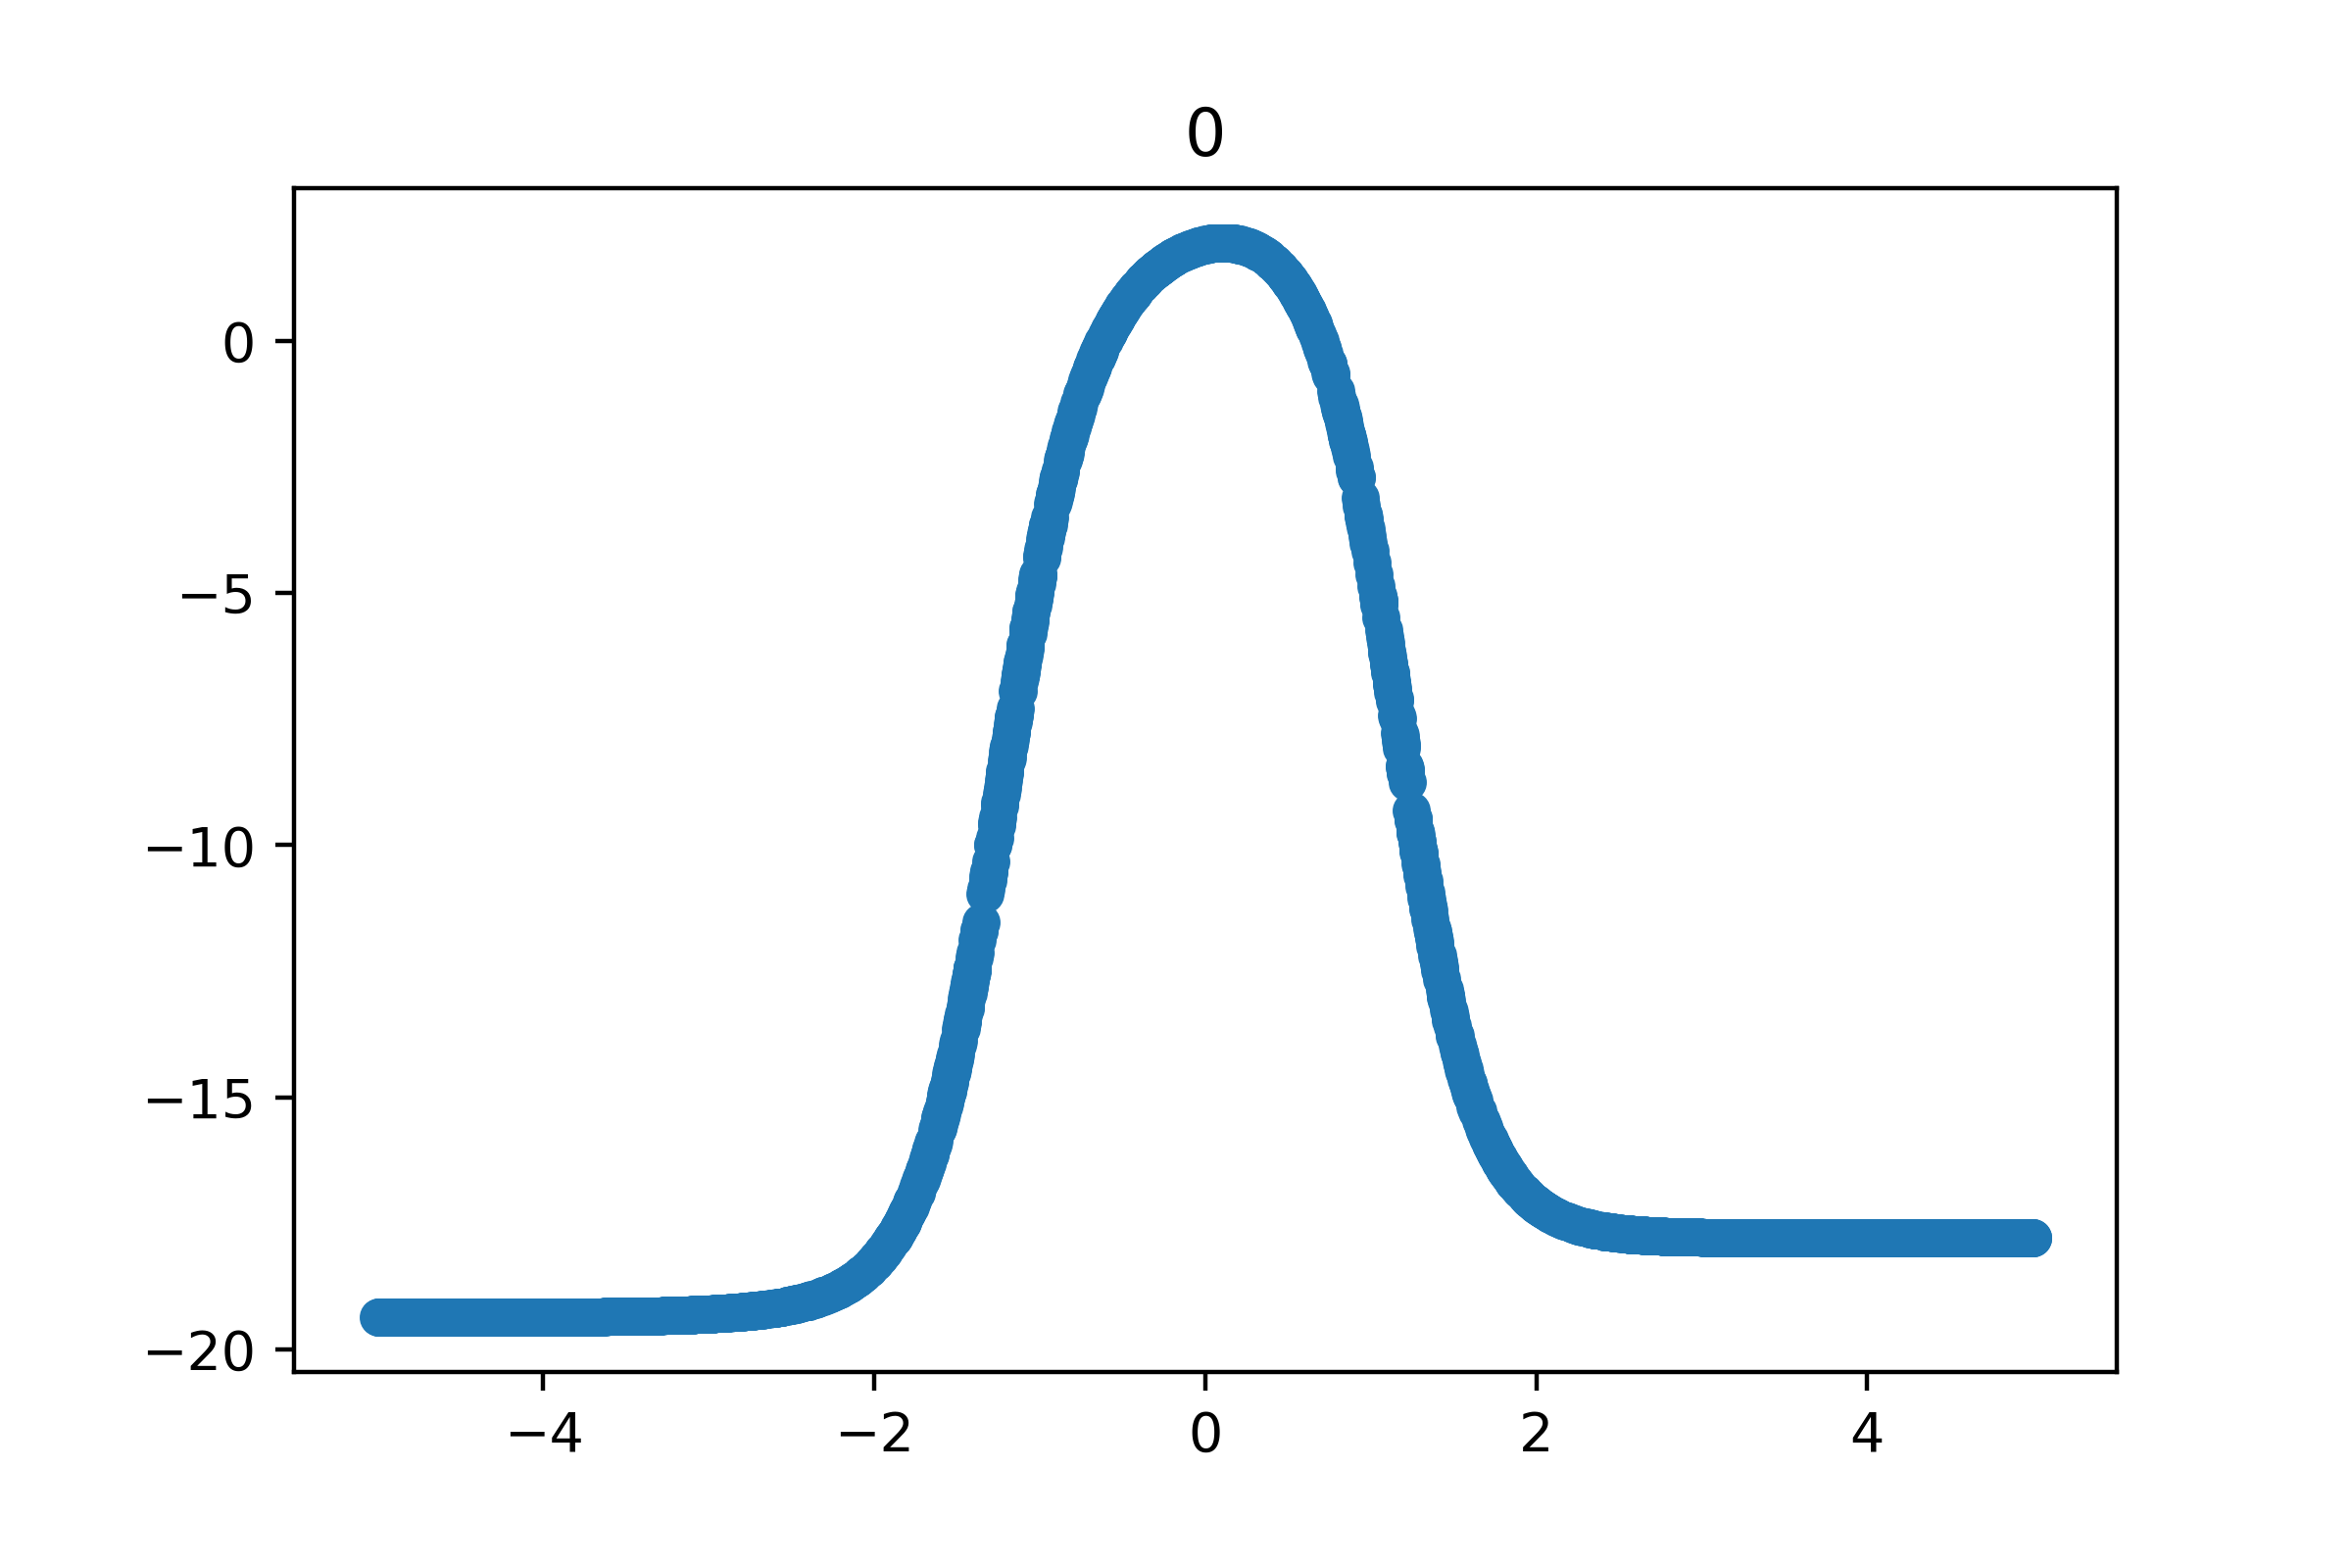
\includegraphics[width=.33\textwidth]{fig/mnl/ci1.png}%
        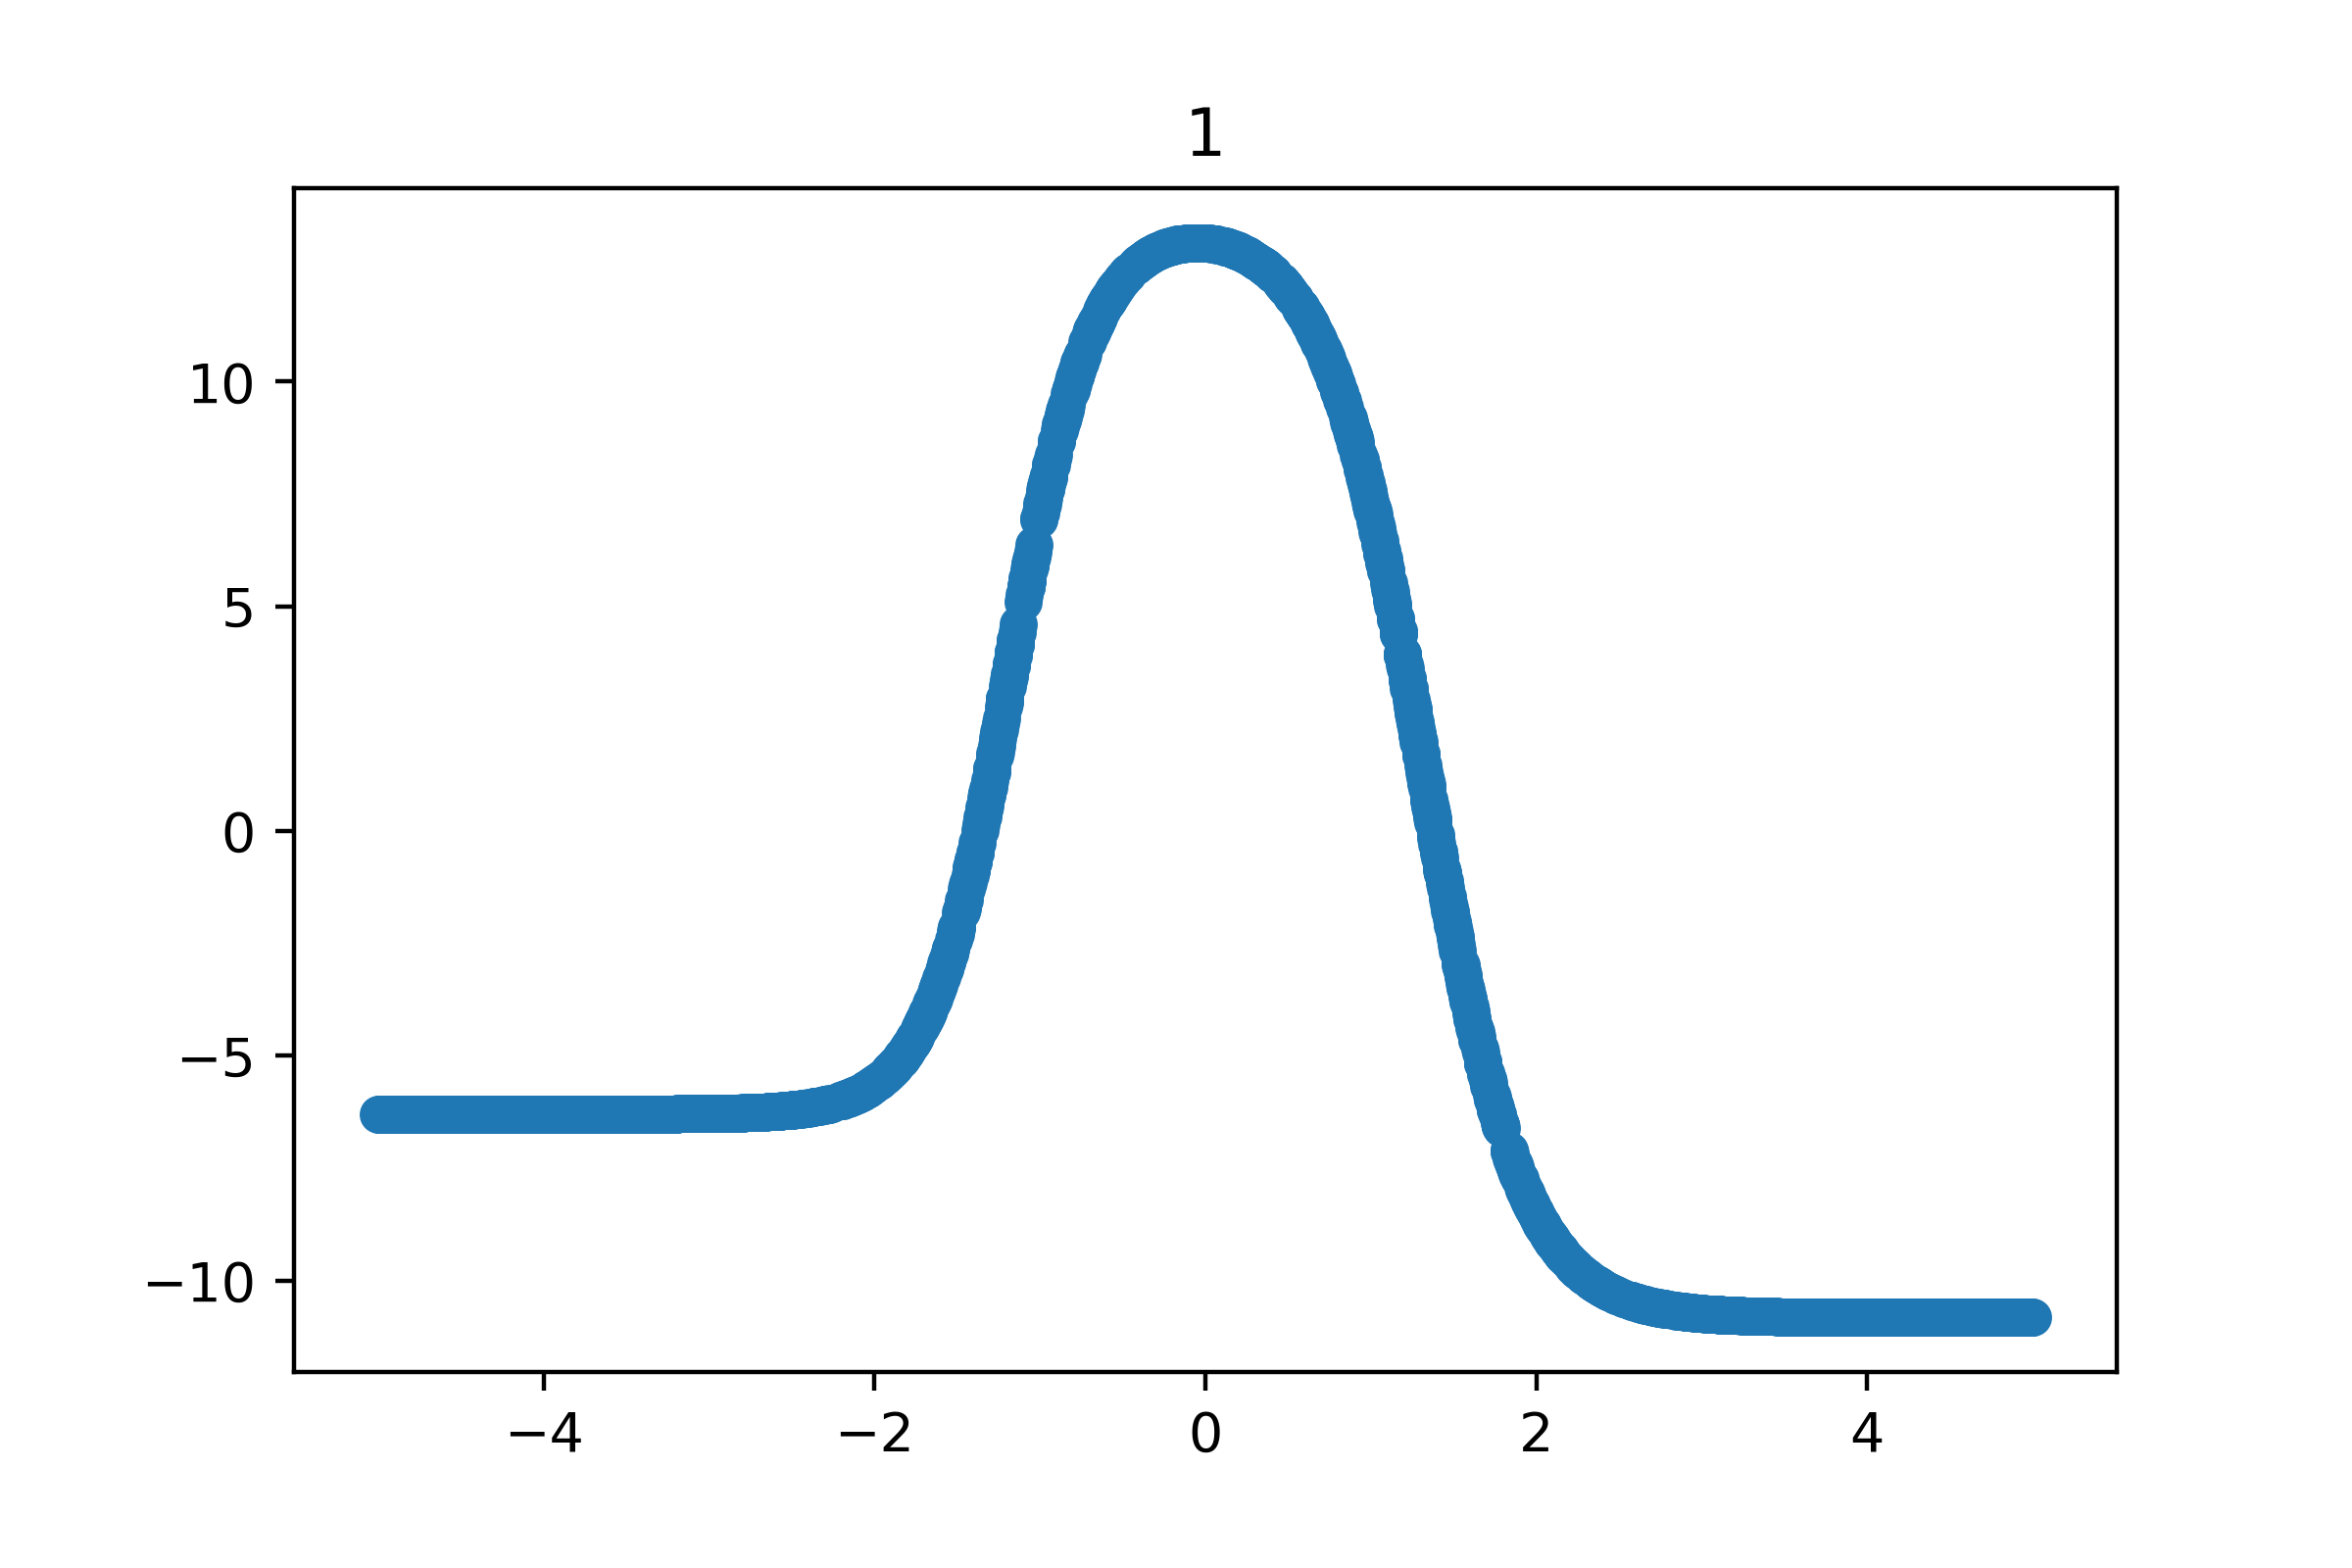
\includegraphics[width=.33\textwidth]{fig/mnl/ci2.png}%
        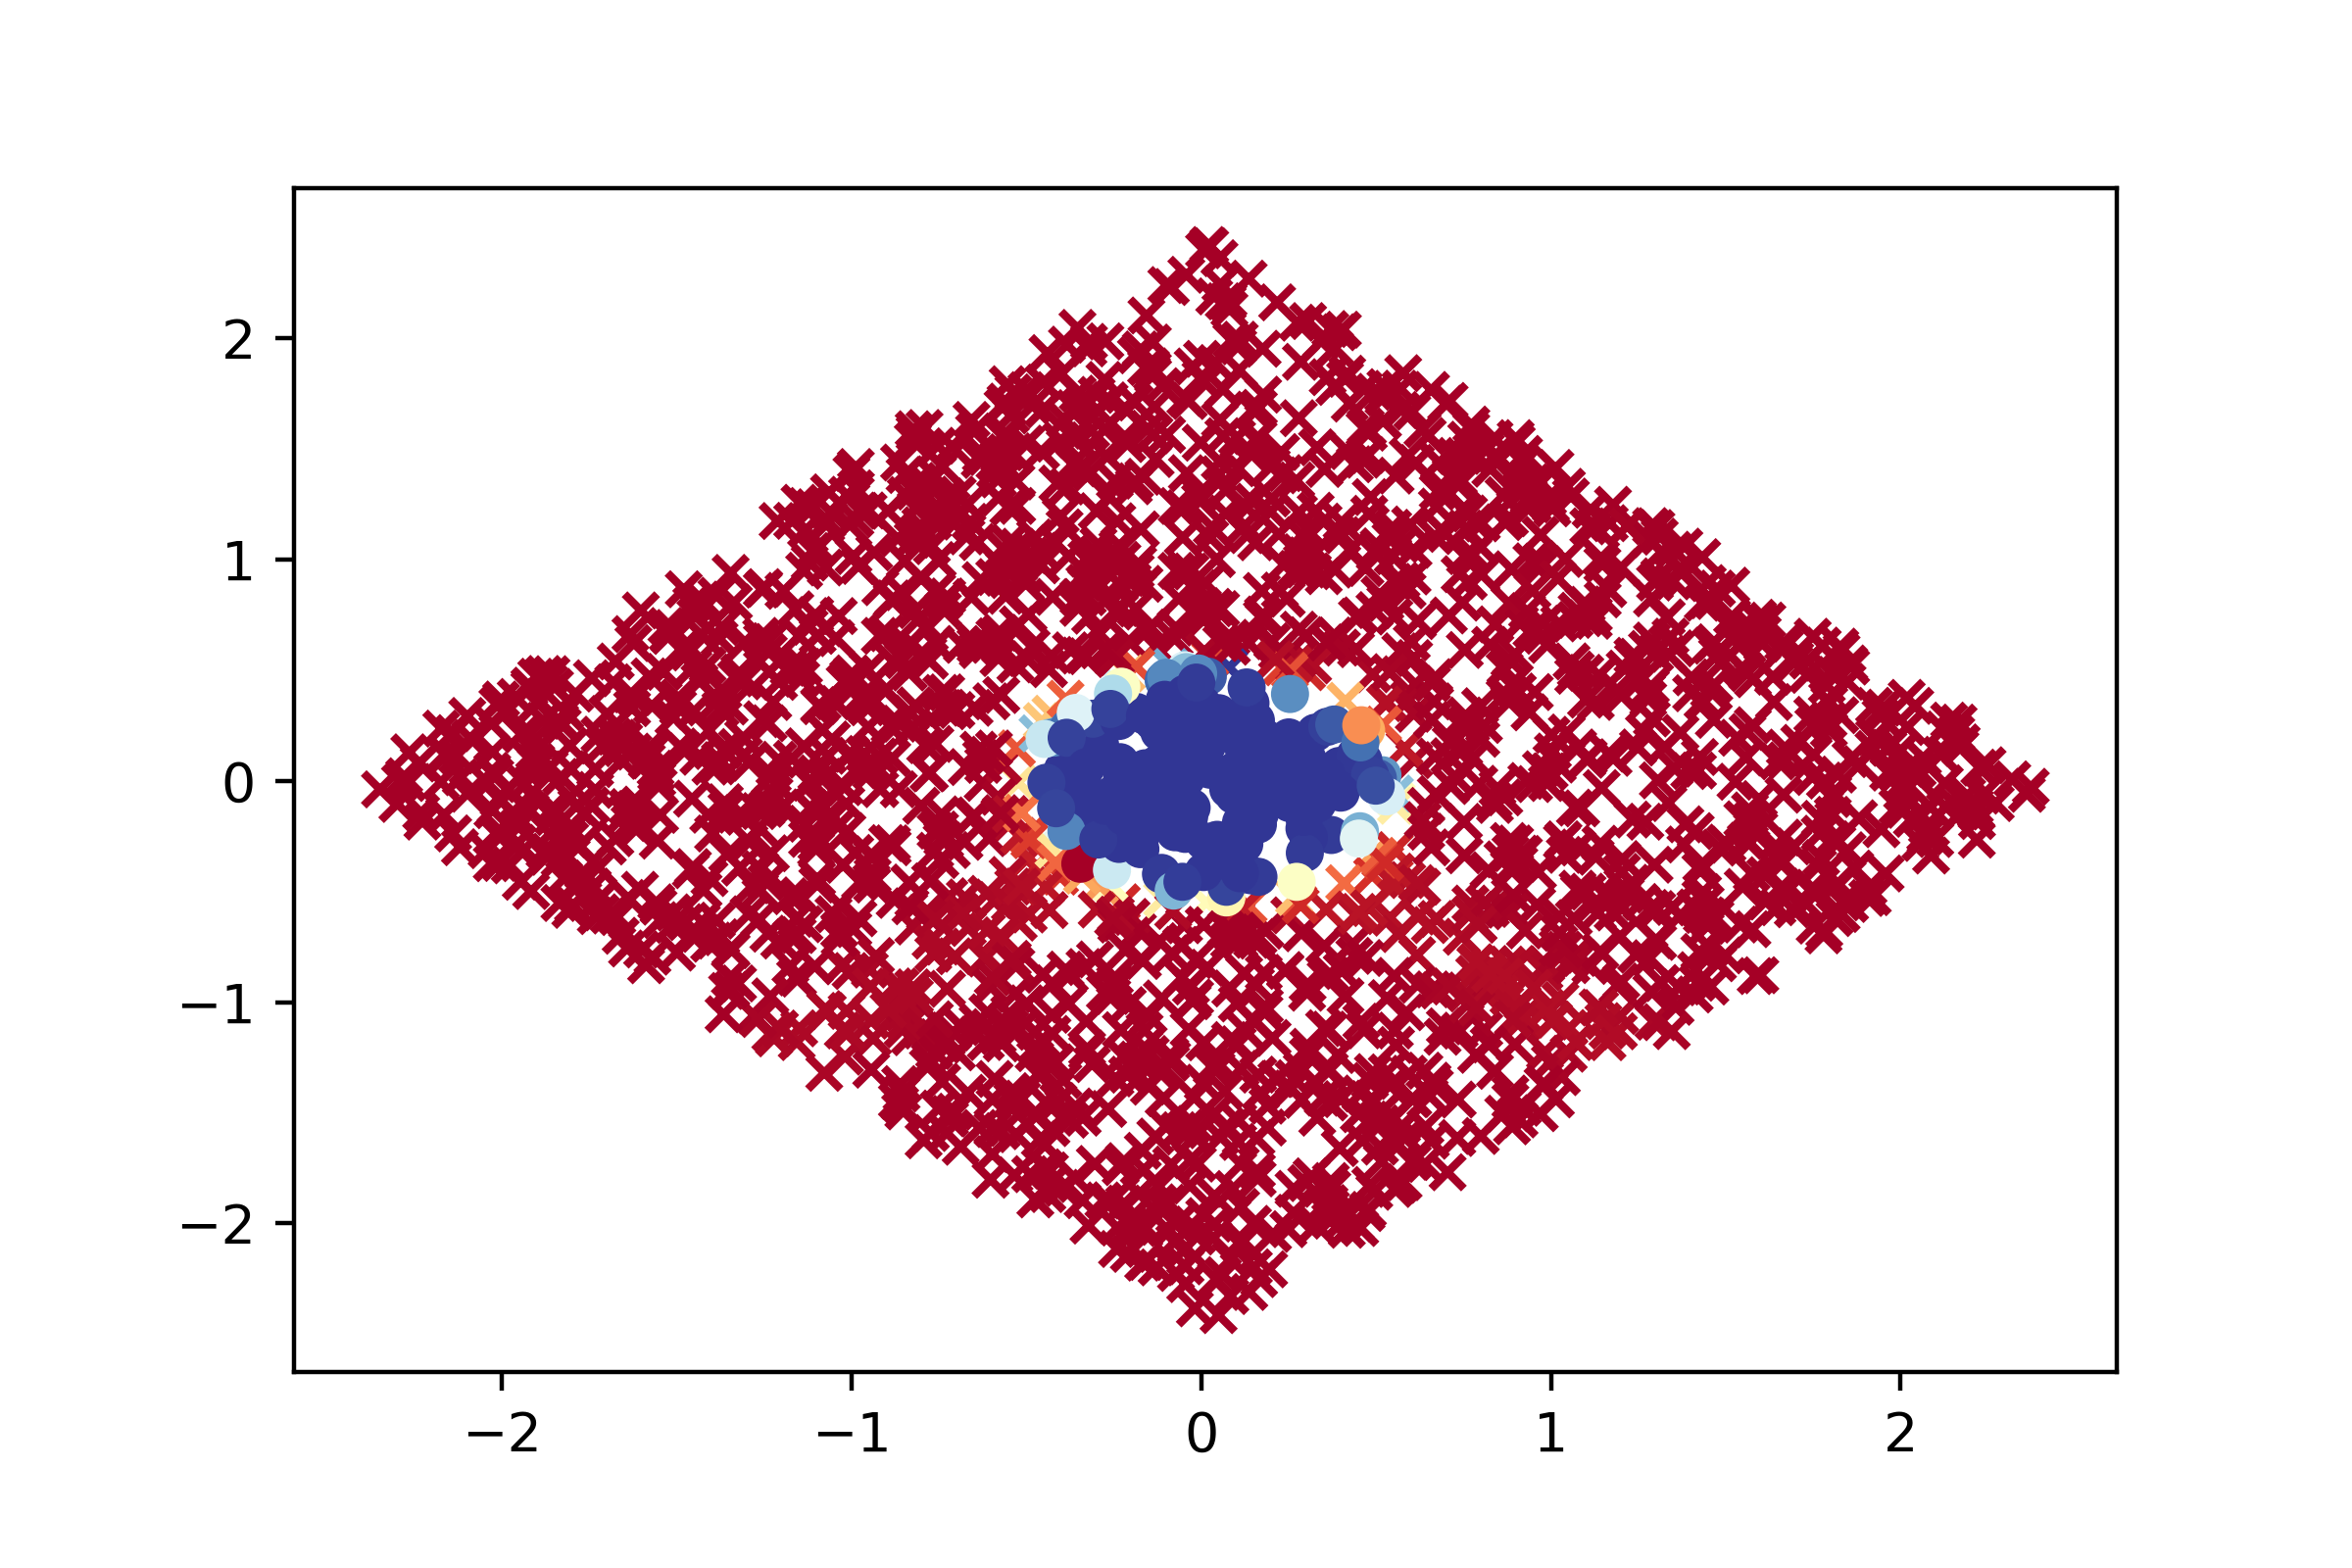
\includegraphics[width=.33\textwidth]{fig/plt/ci.png}
        \caption{Circle Dataset}
    \end{subfigure}
    \begin{subfigure}{1.0\textwidth}
        \centering
        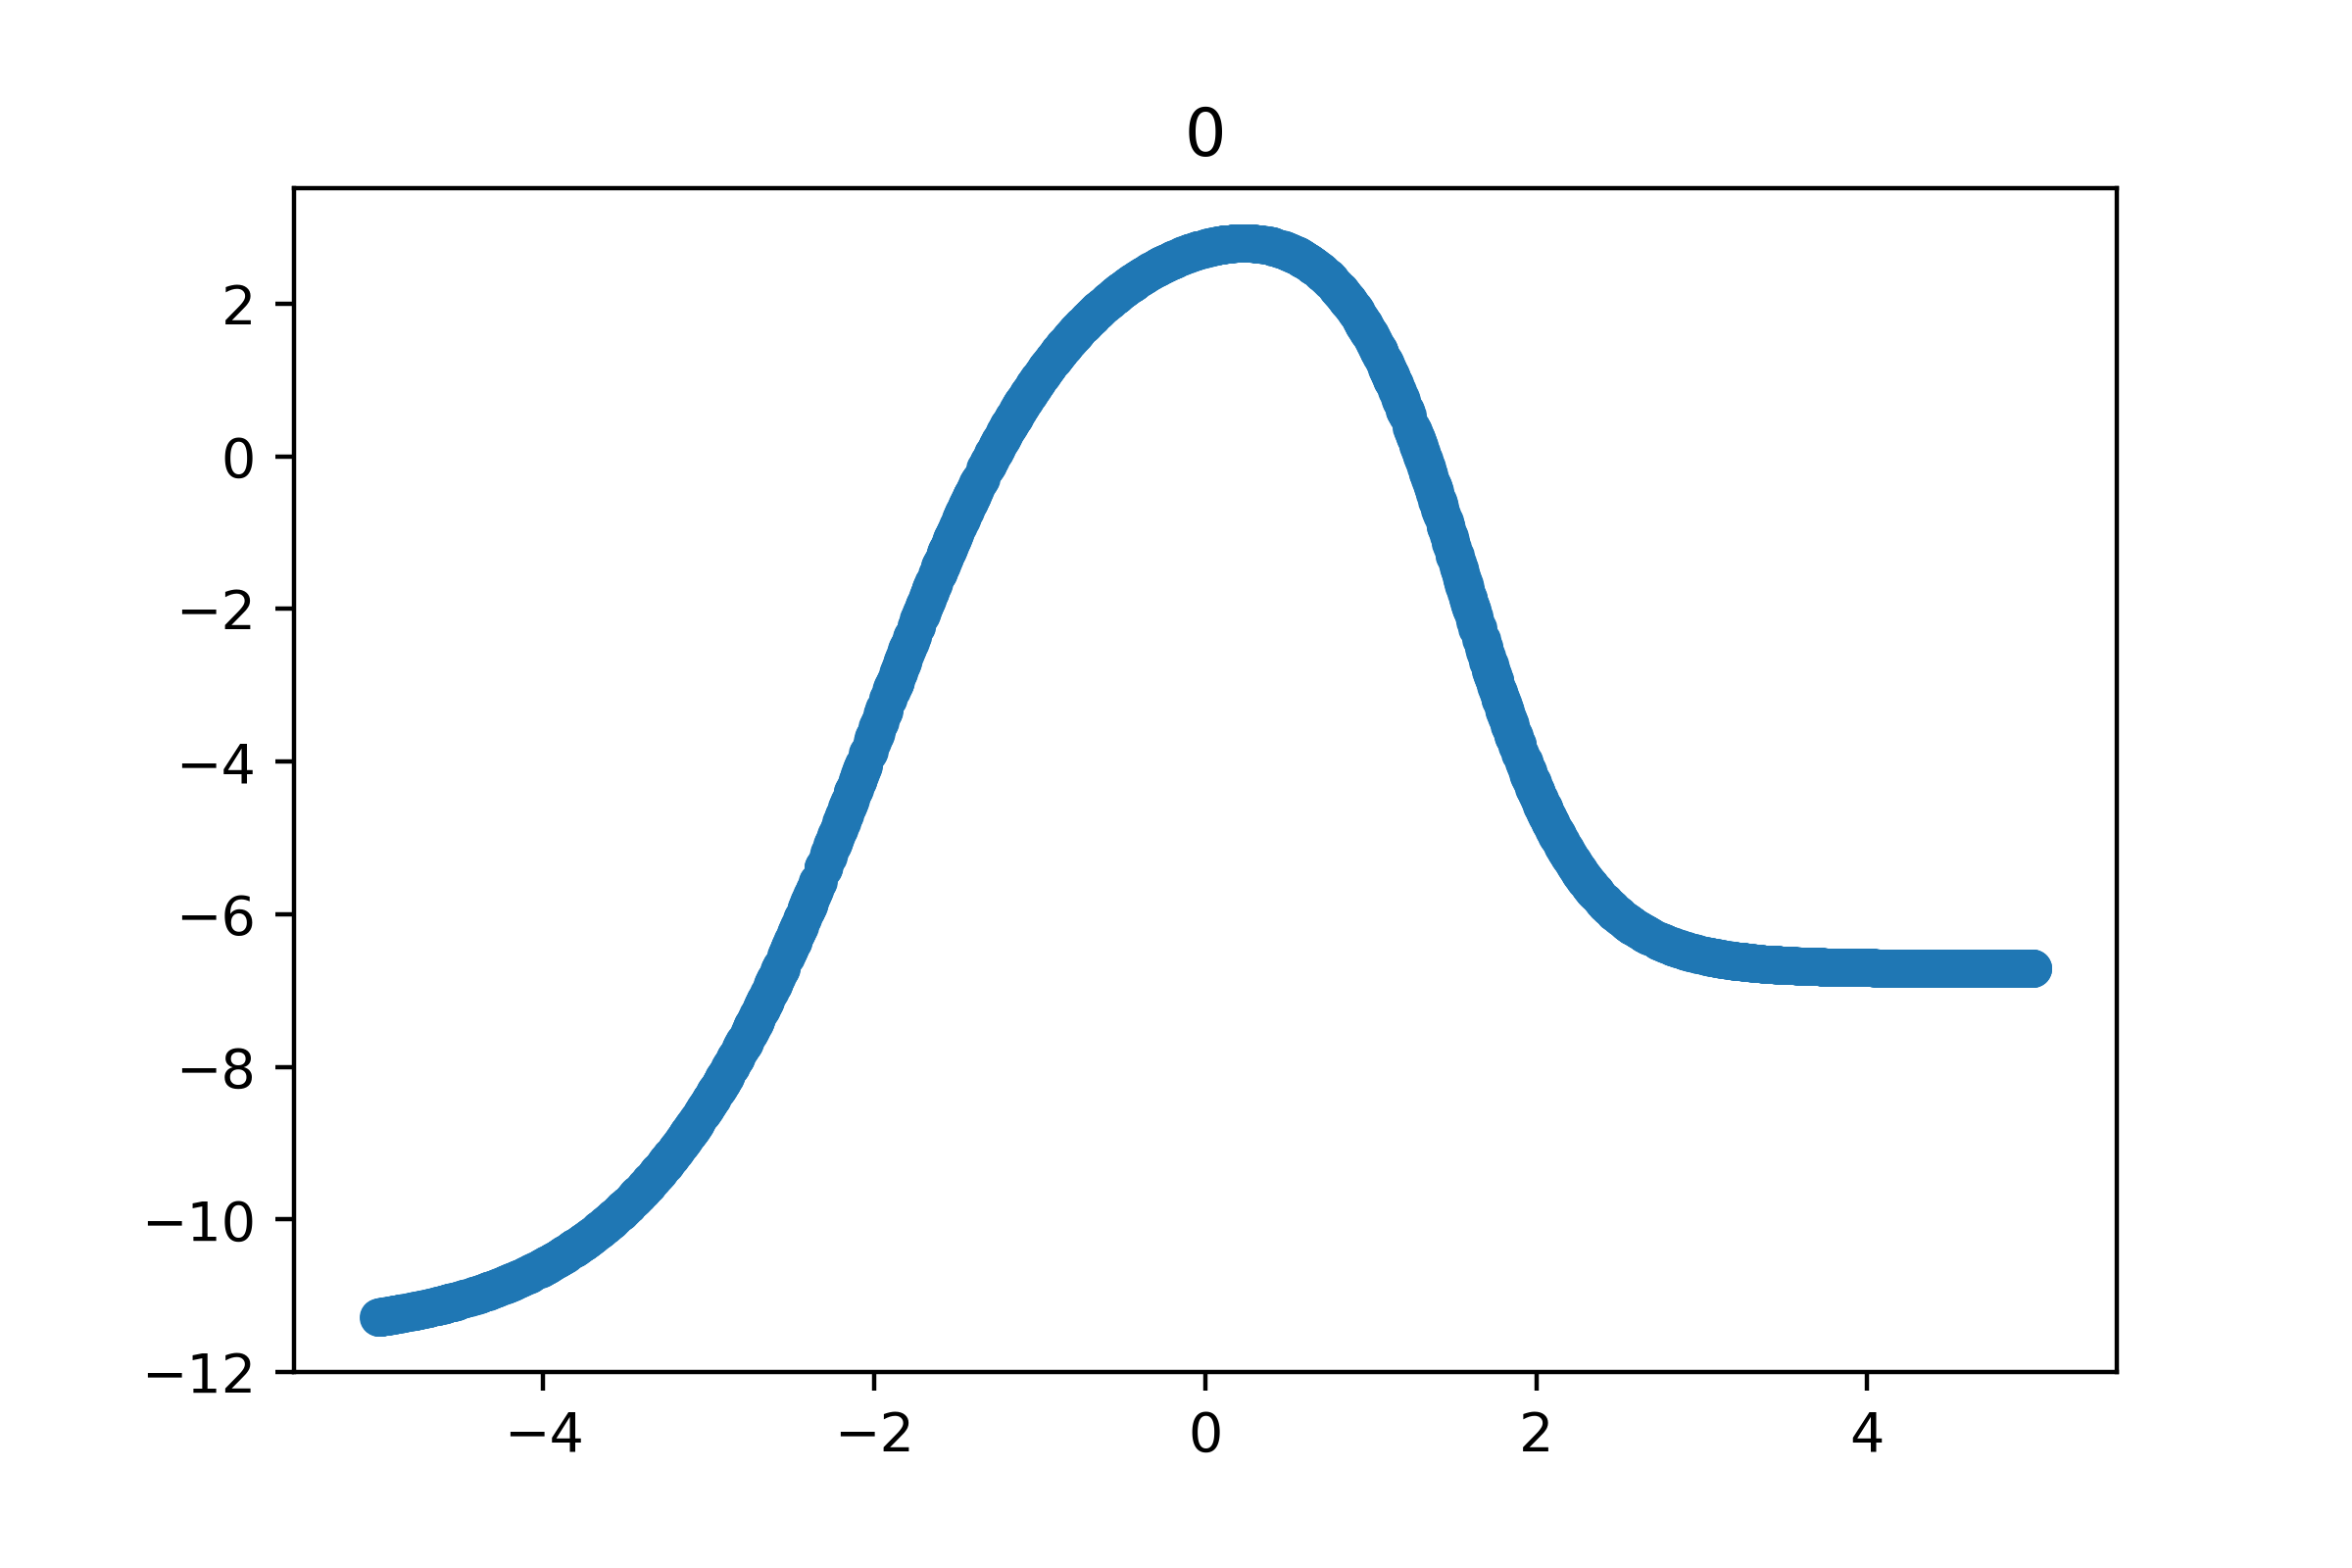
\includegraphics[width=.33\textwidth]{fig/mnl/el1.png}%
        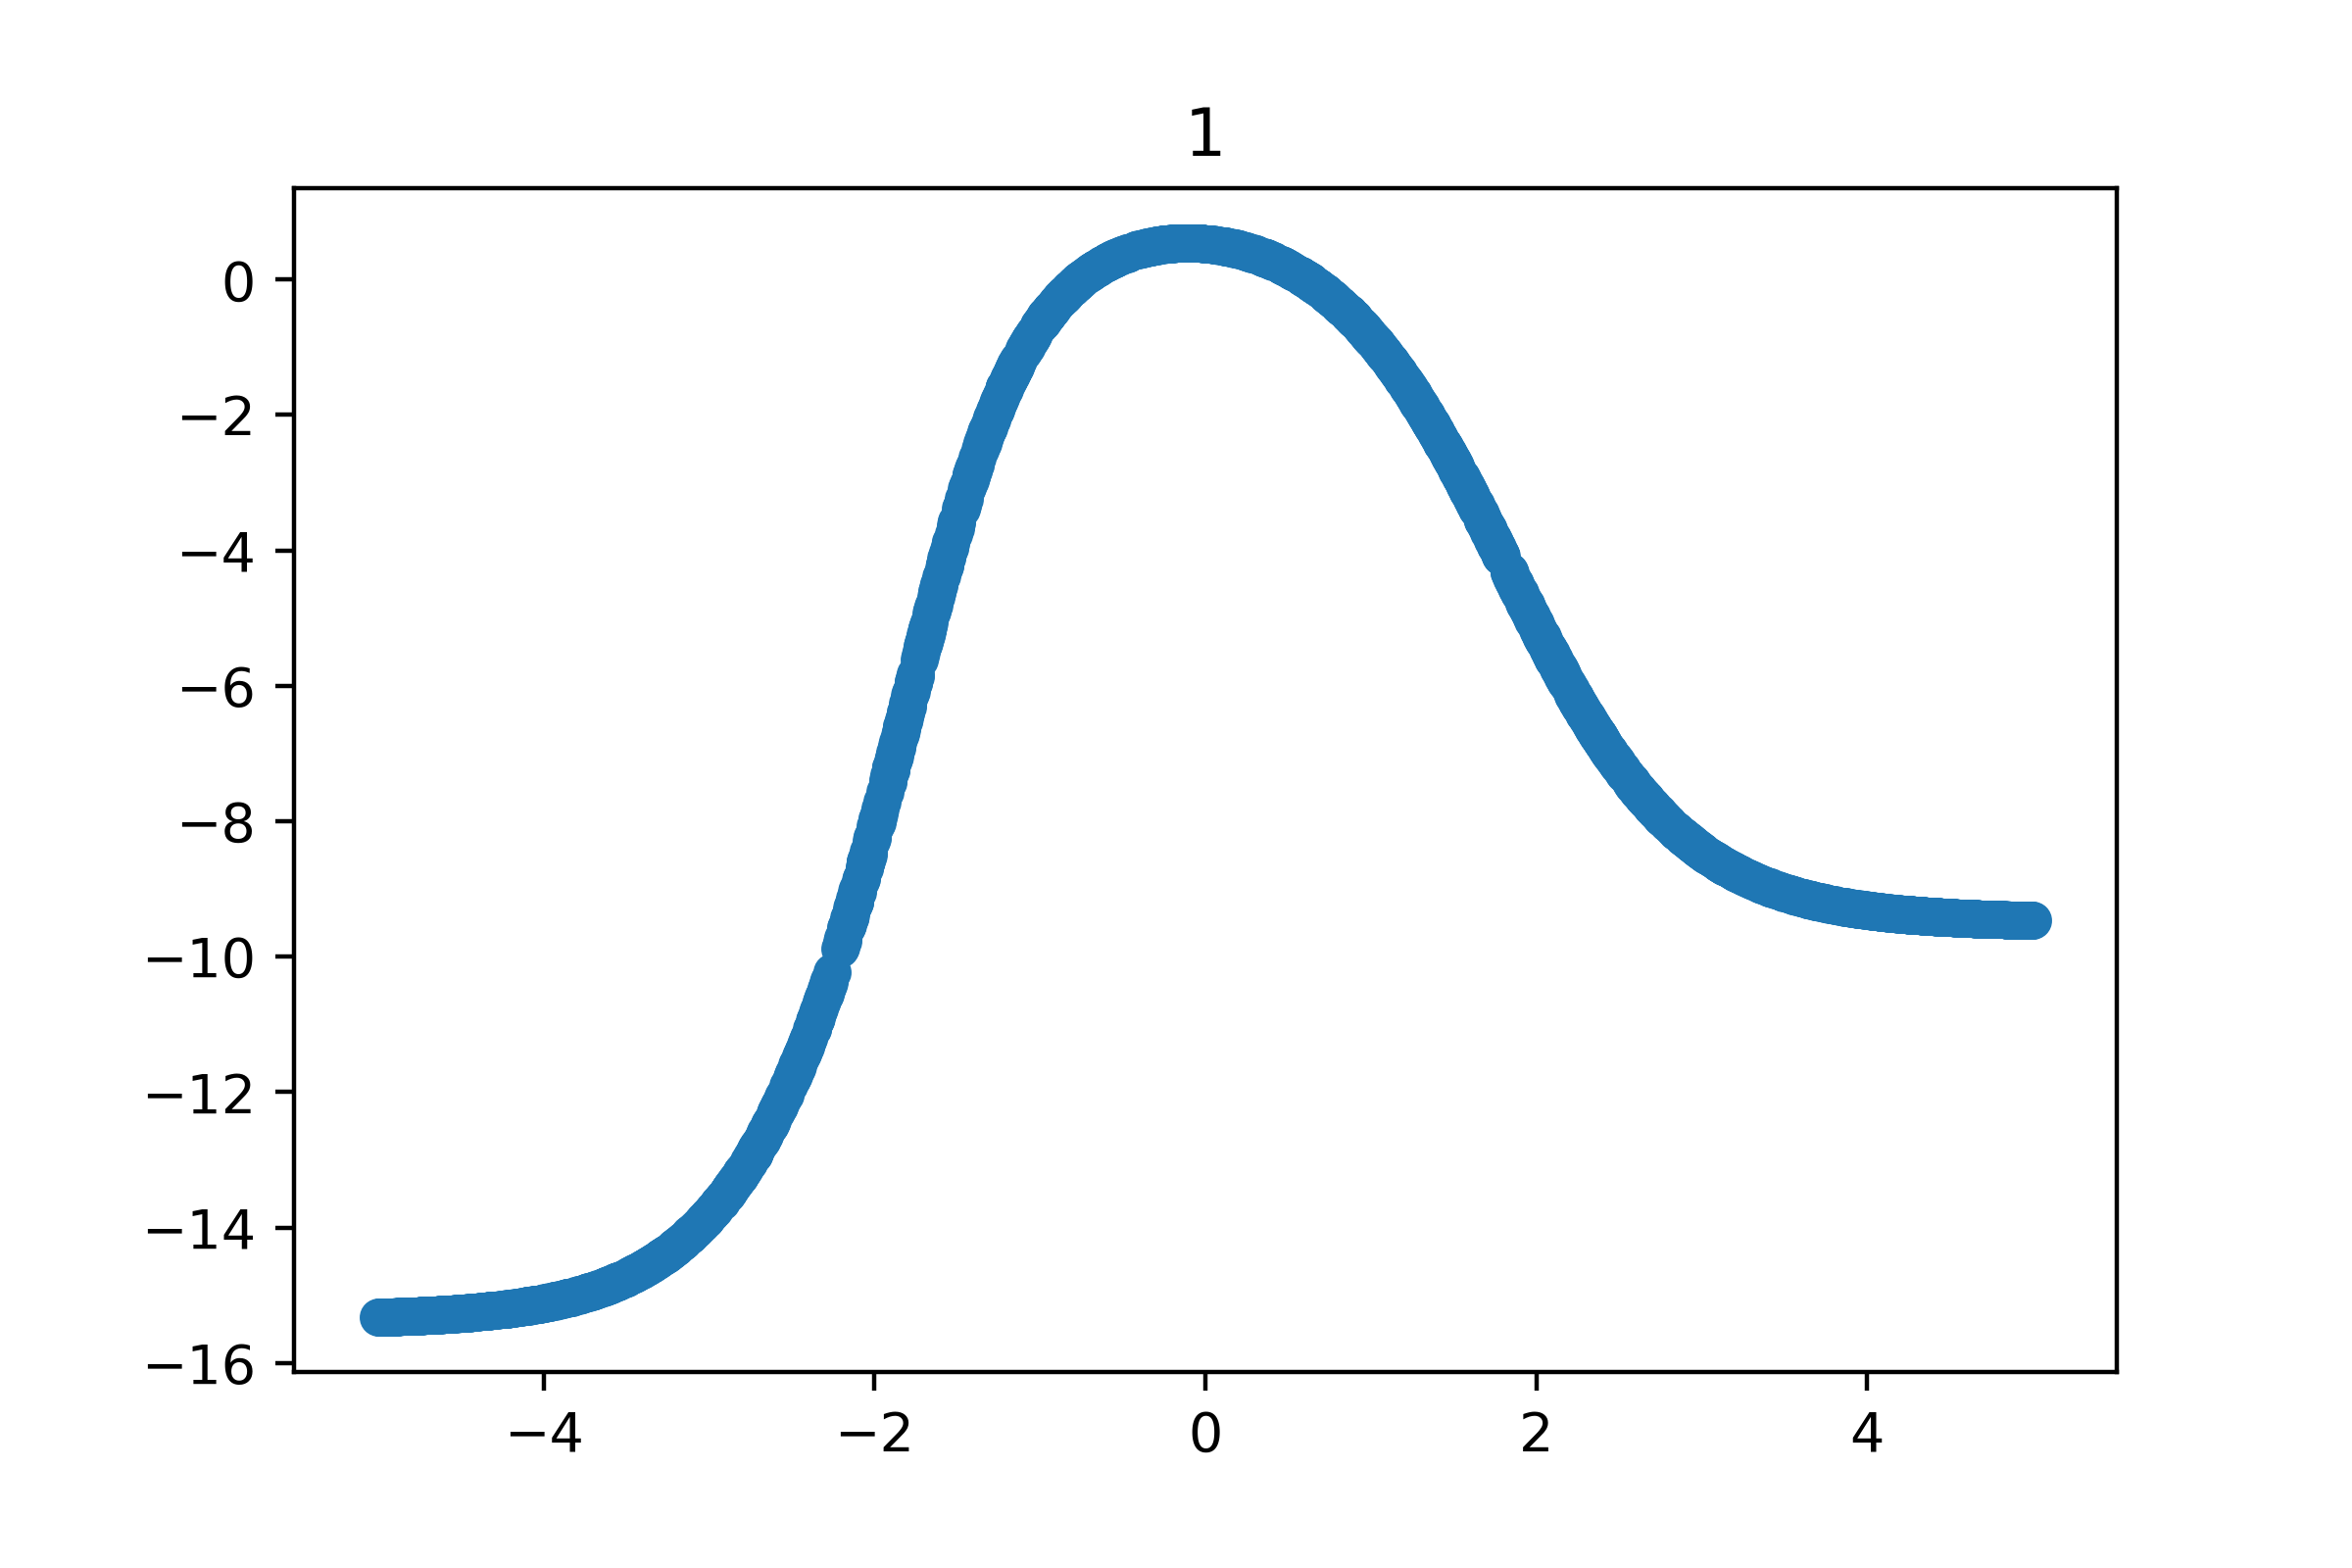
\includegraphics[width=.33\textwidth]{fig/mnl/el2.png}%
        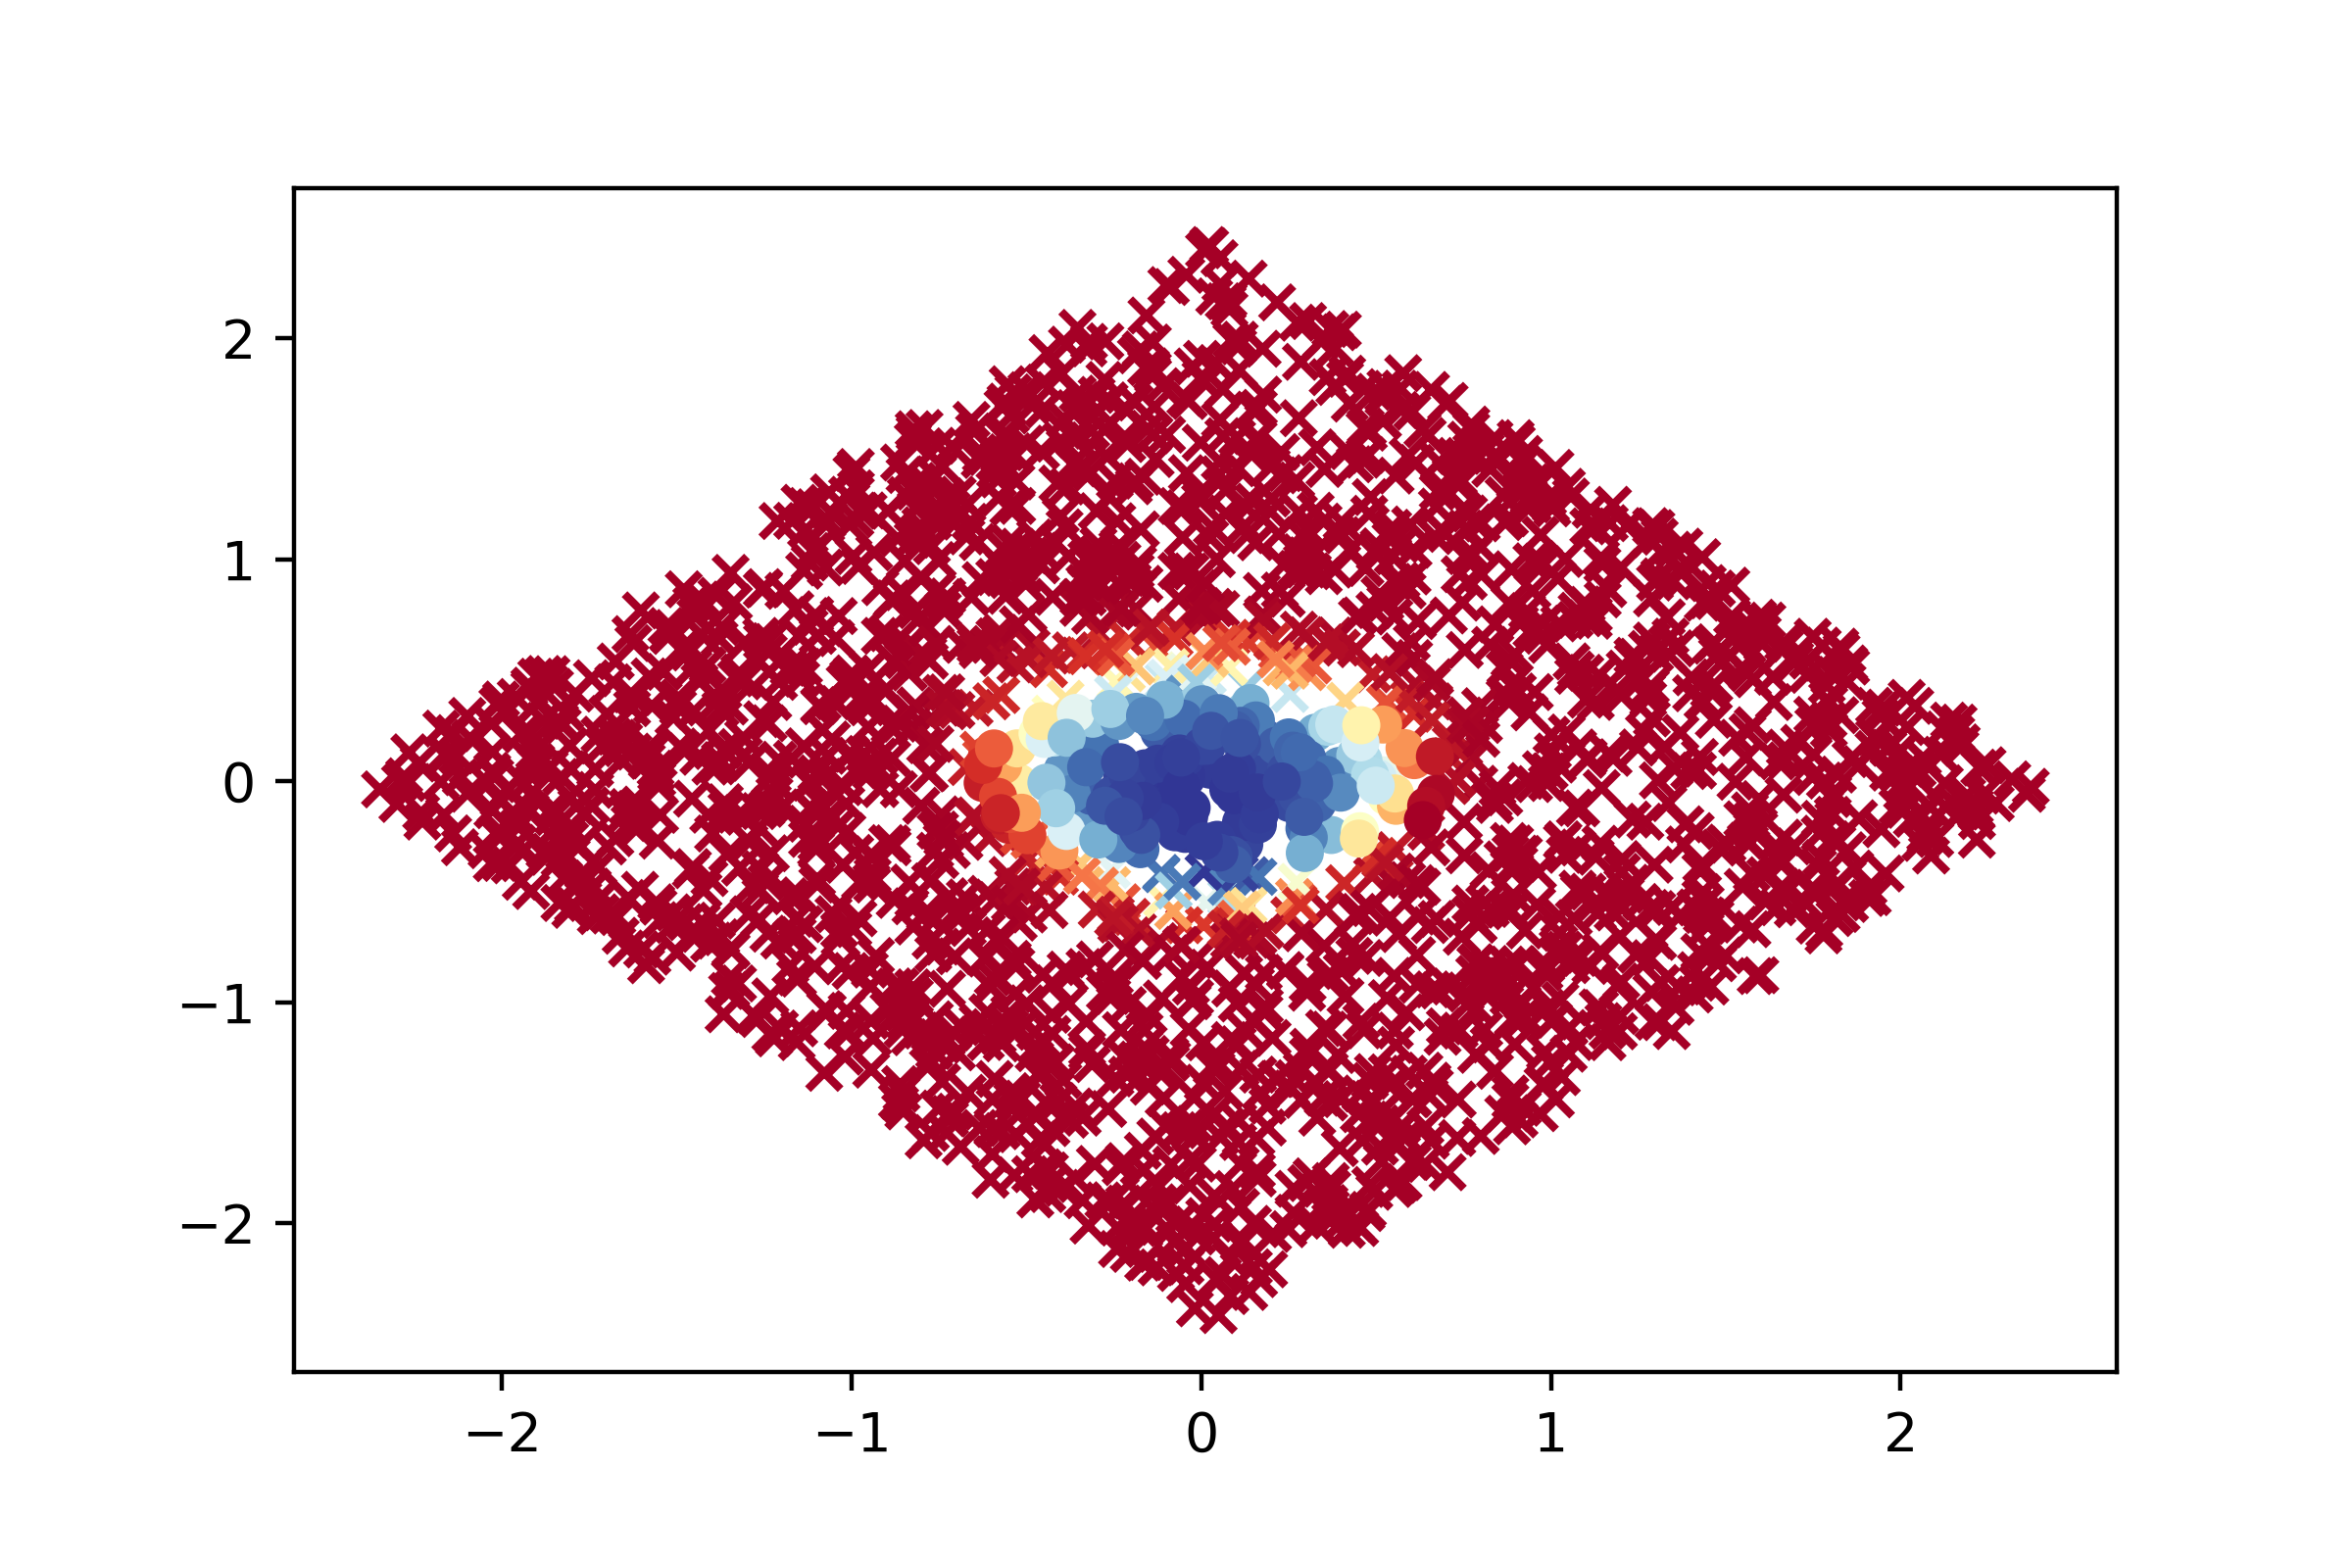
\includegraphics[width=.33\textwidth]{fig/plt/el.png}
        \caption{Ellipse Dataset}
    \end{subfigure}
    \begin{subfigure}{1.0\textwidth}
        \centering
        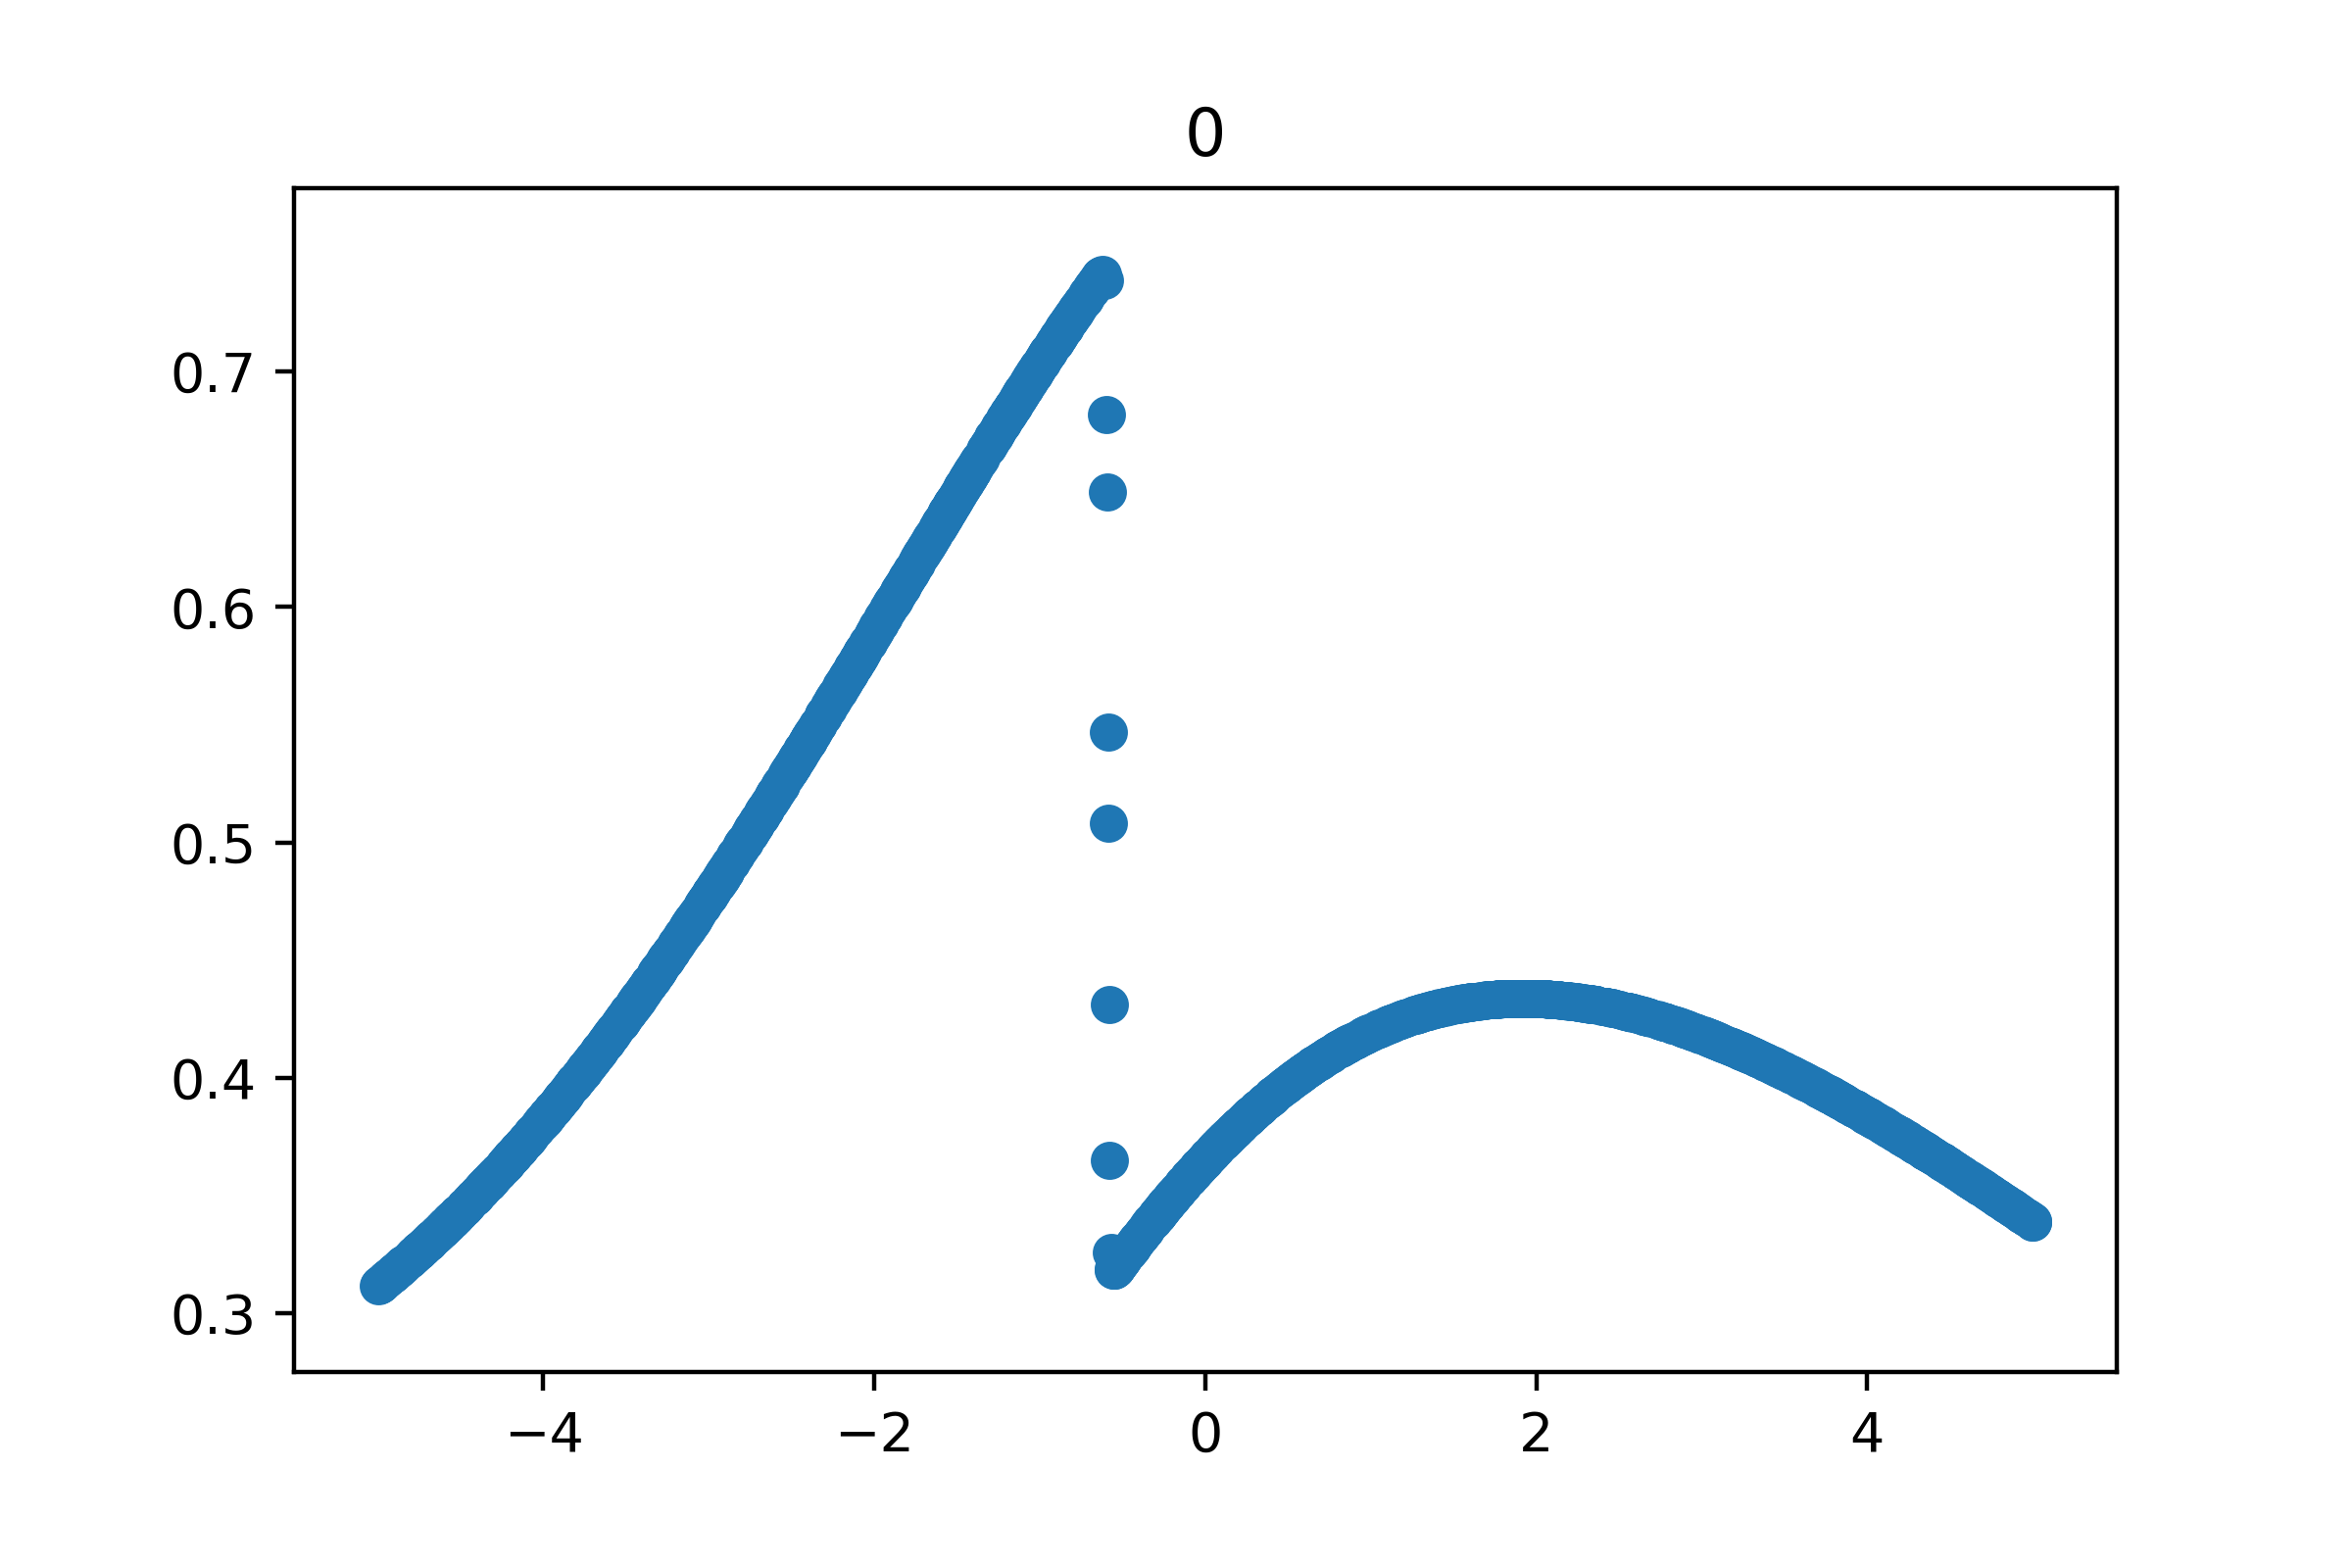
\includegraphics[width=.33\textwidth]{fig/mnl/xr1.png}%
        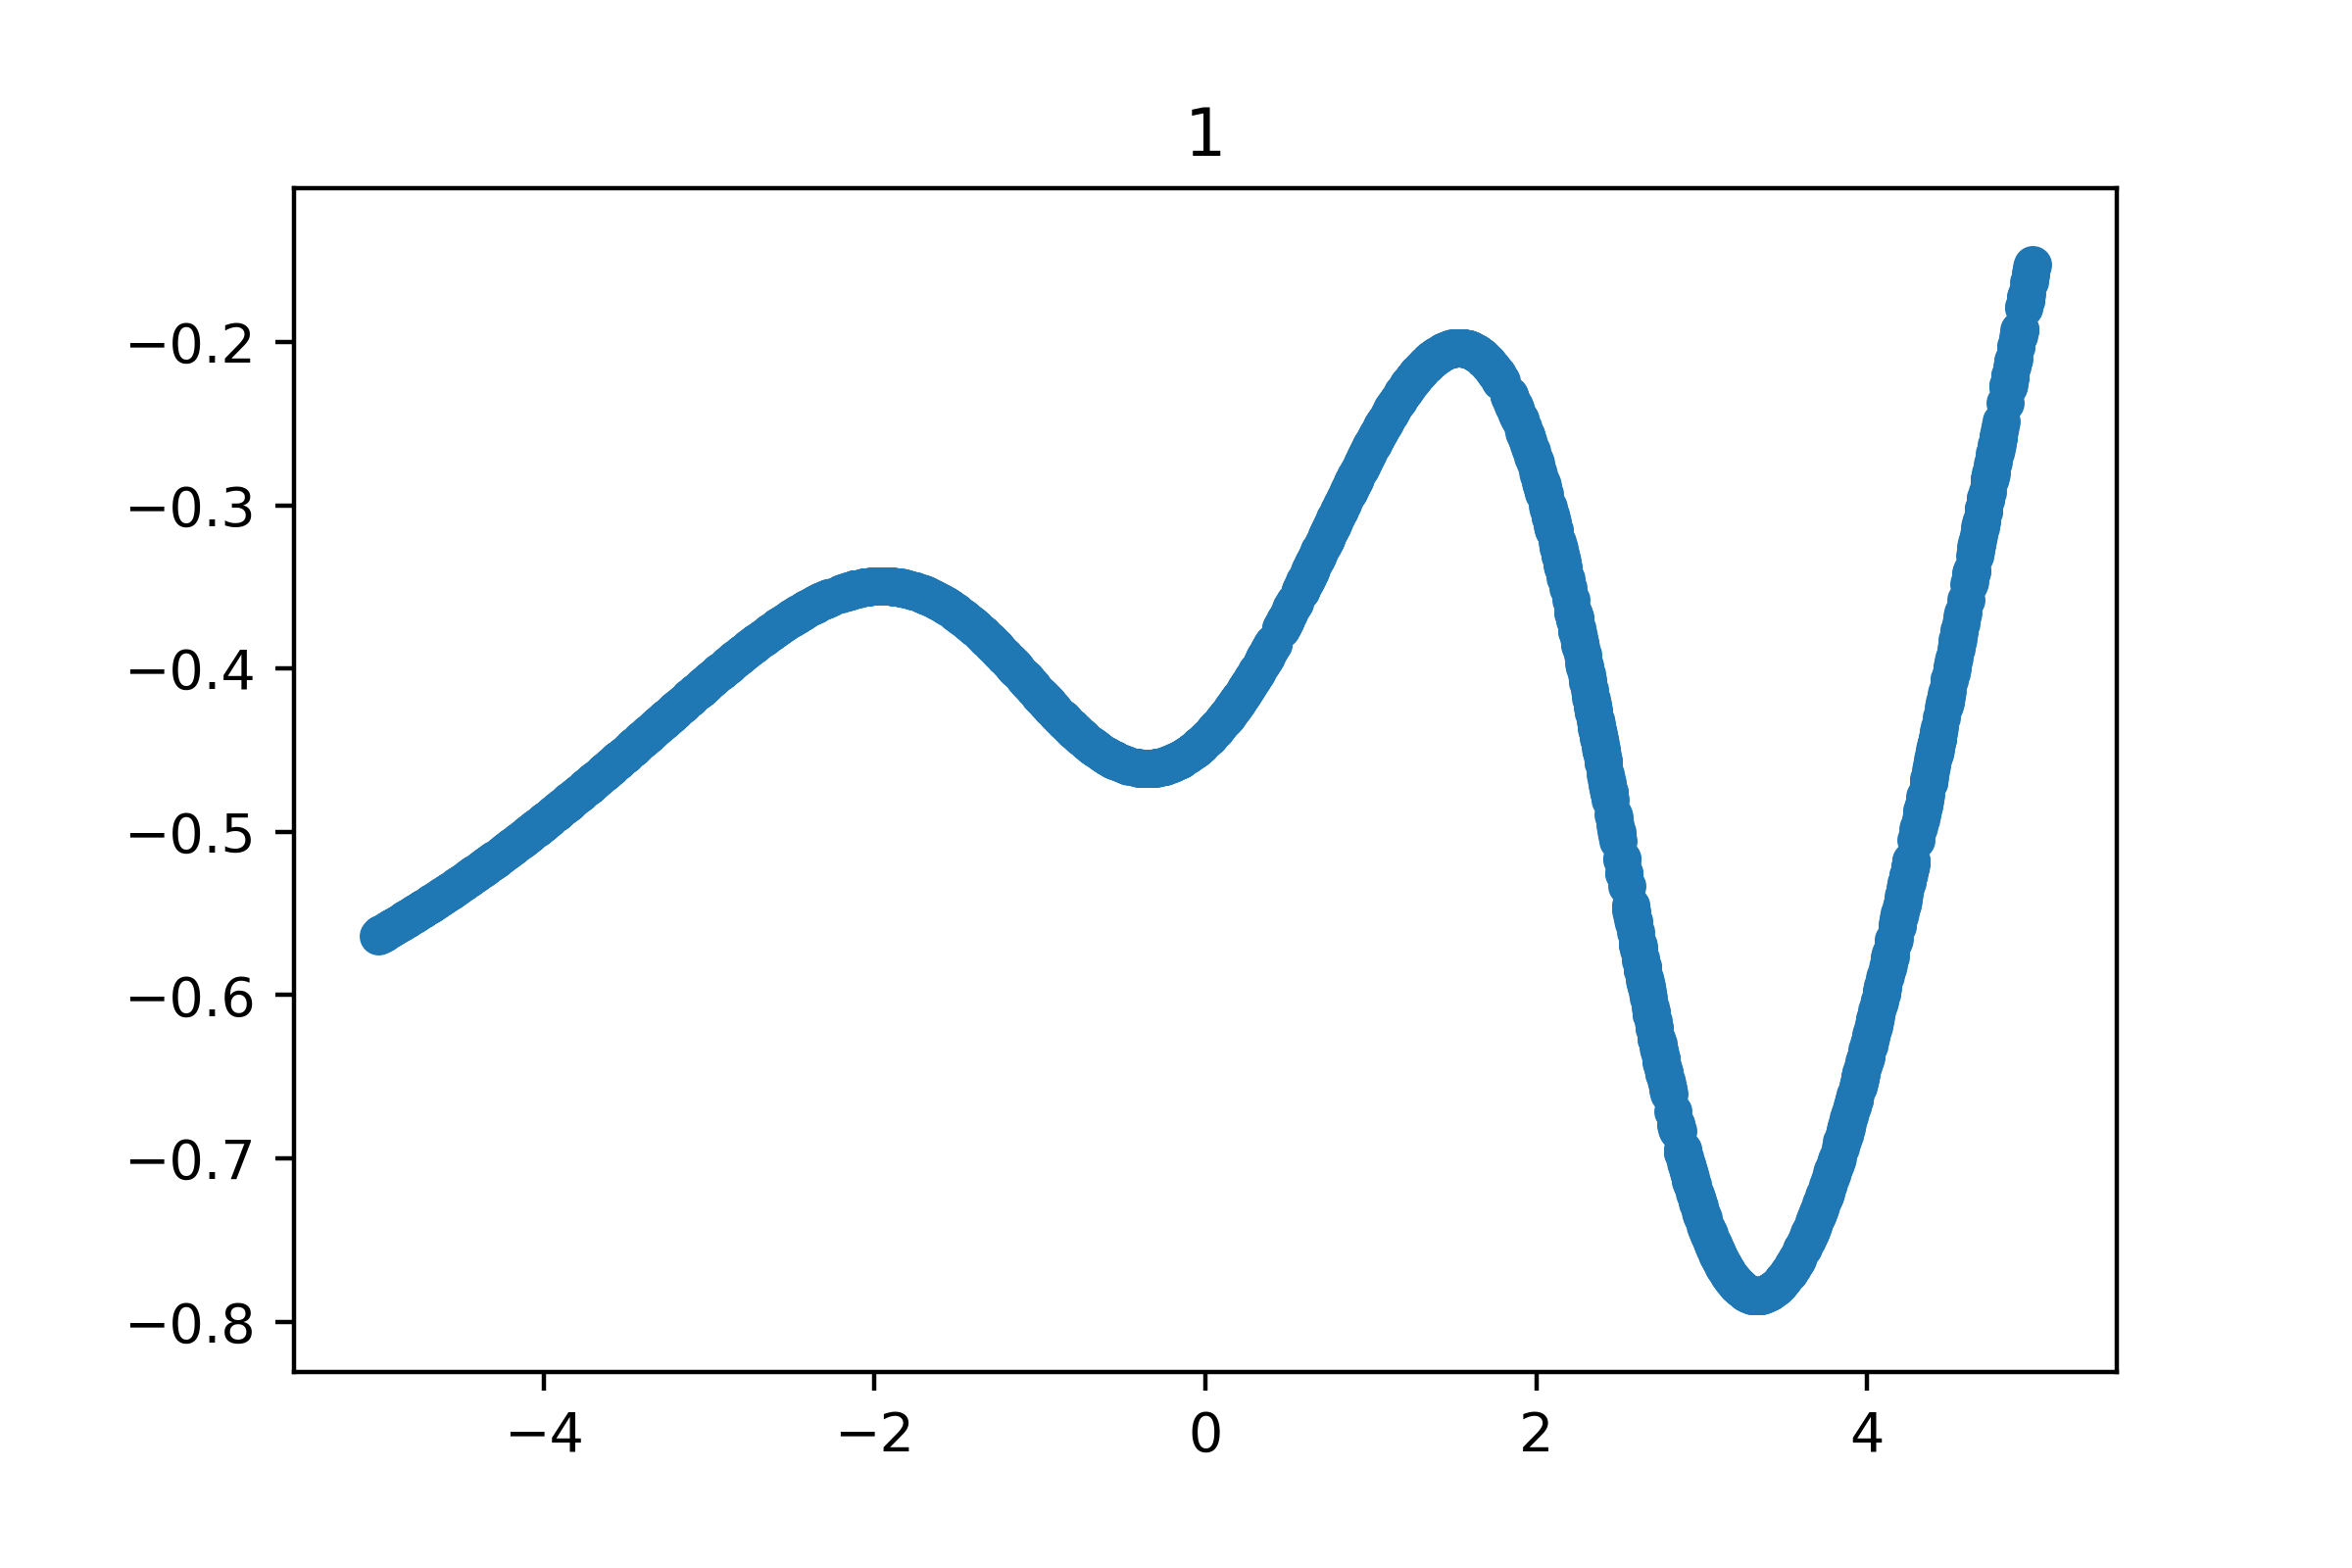
\includegraphics[width=.33\textwidth]{fig/mnl/xr2.png}%
        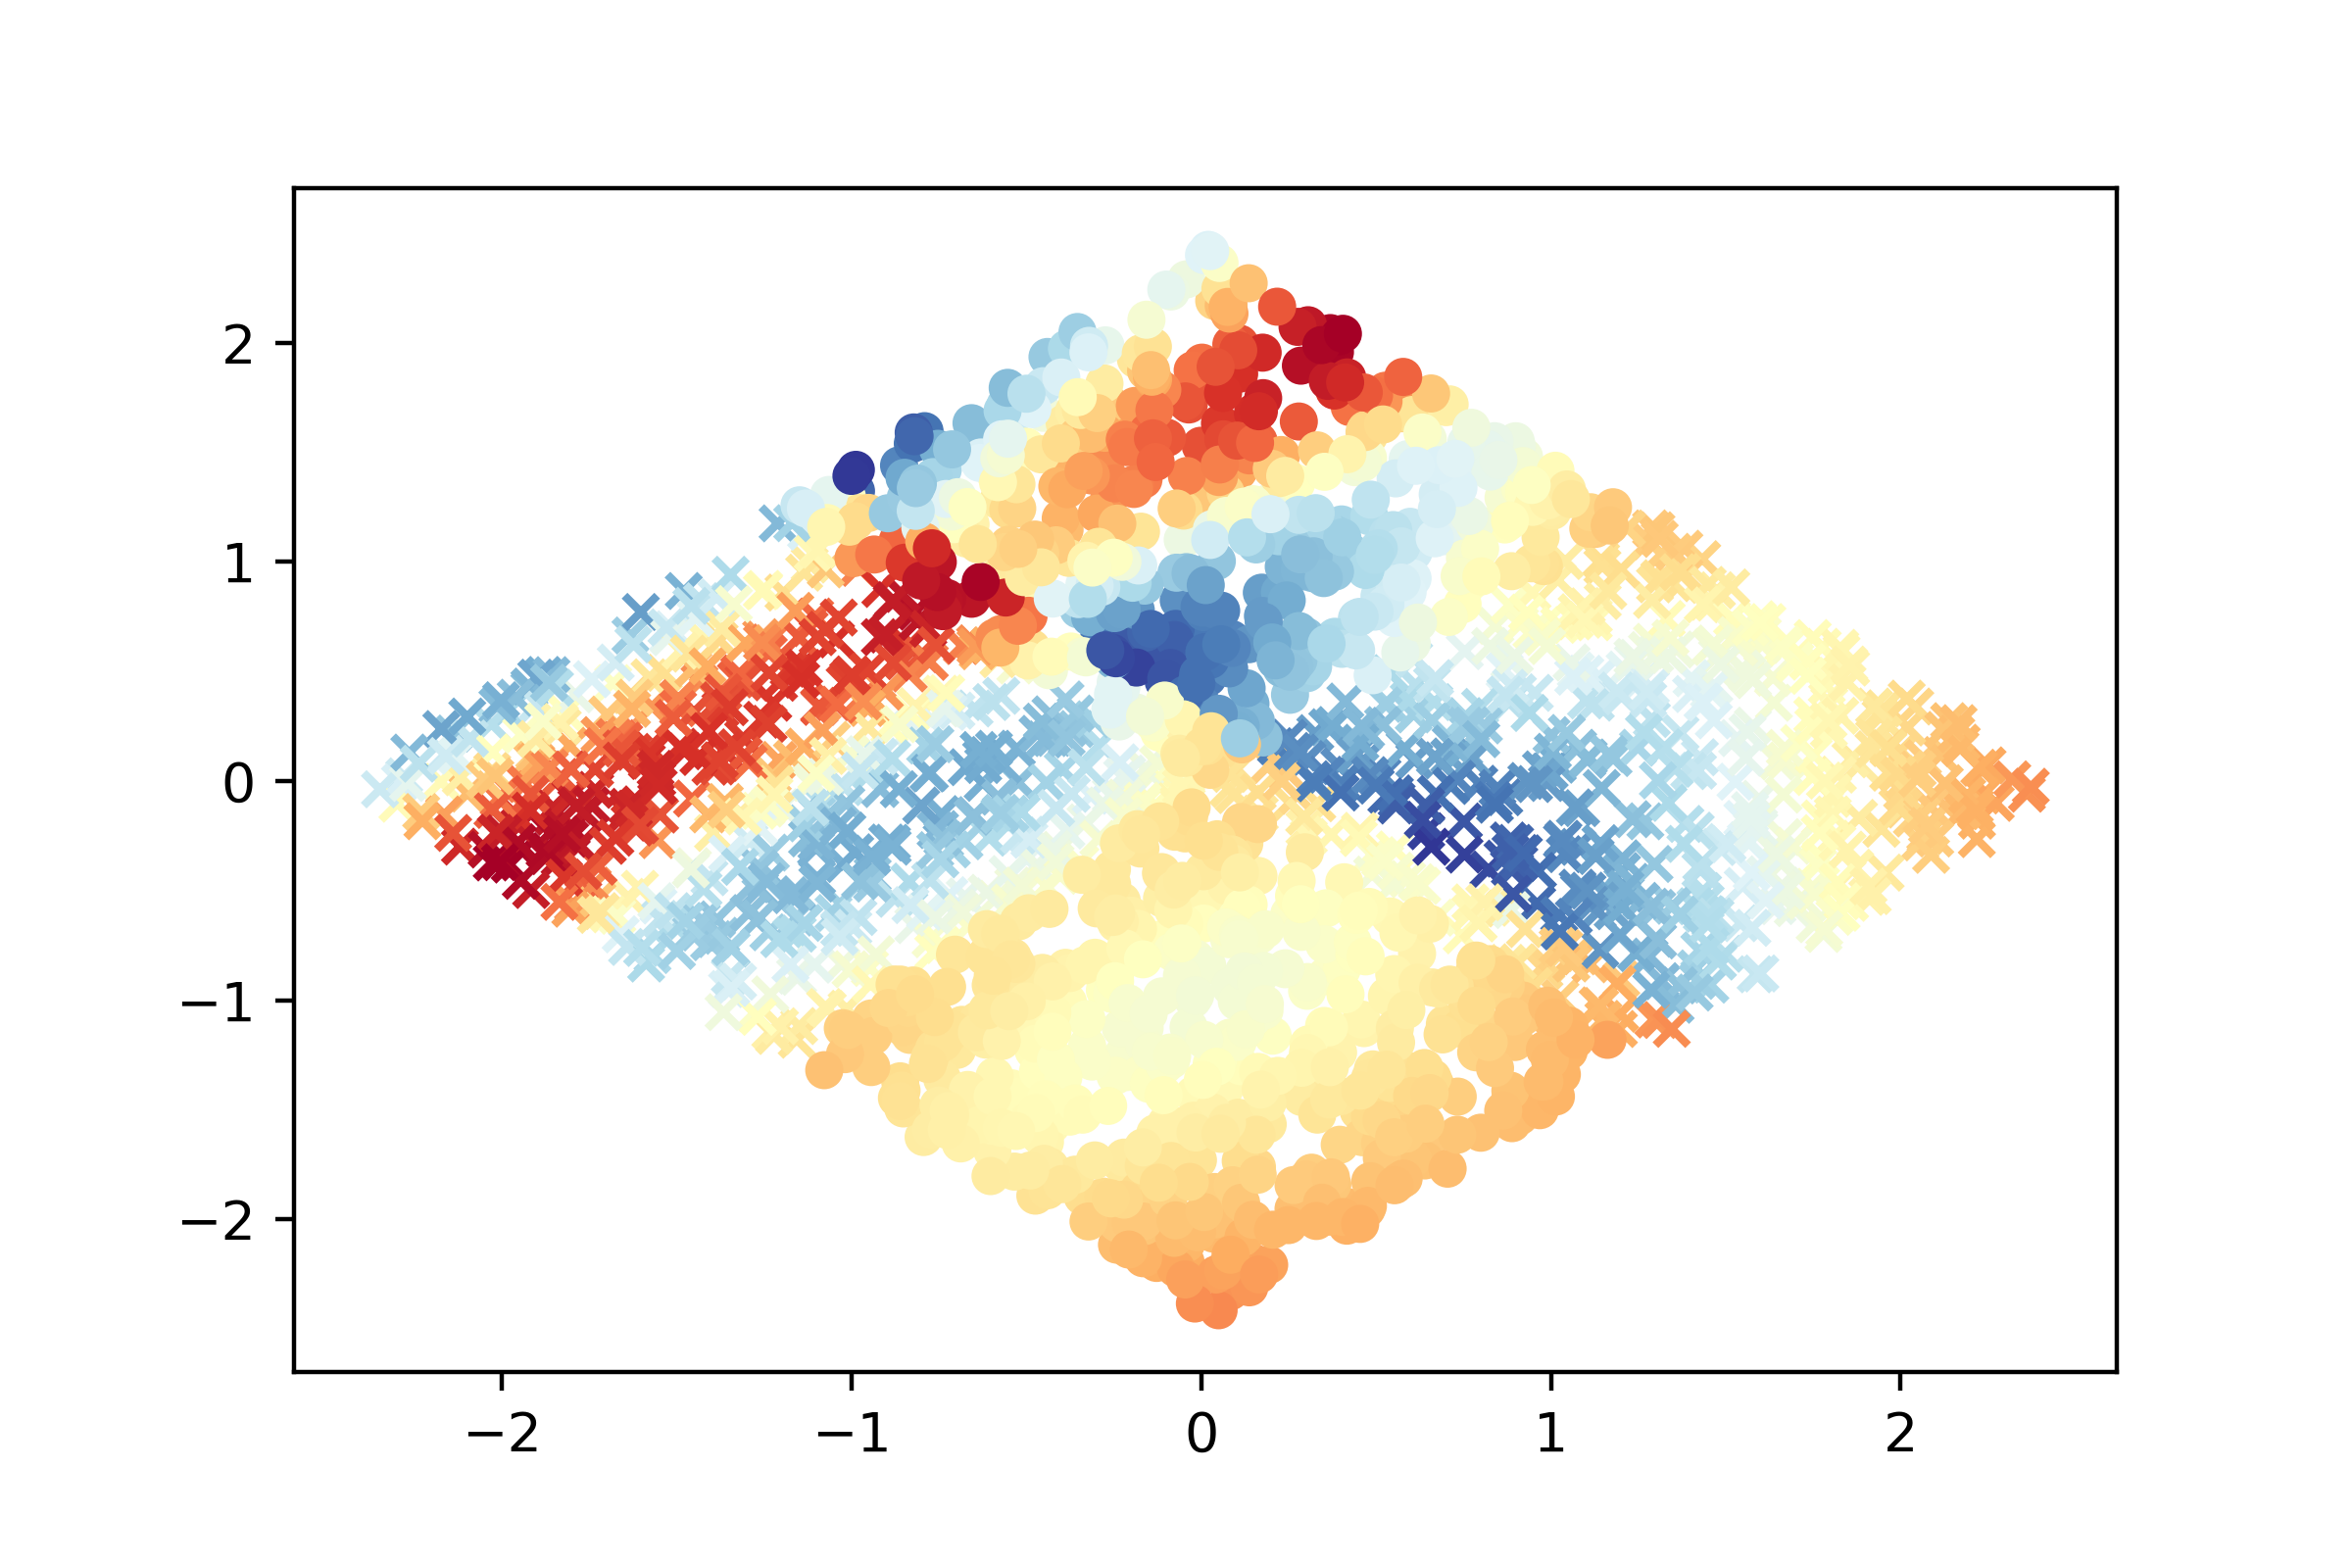
\includegraphics[width=.33\textwidth]{fig/plt/xr.png}
        \caption{XOR Dataset}
    \end{subfigure}
    \caption{Network predictions and selection of marginals for each dataset. In the first two columns (marginals), the x-axis represents the domain on the input variable and the y-axis represents the pre-sigmoid contribution to the response. In the third column, network predictions are presented as two-dimensional principle components plots. X's are true negatives and O's are true positives. Colors represent the network prediction, with blue being positive, red being negative, and yellow being neutral.}
    \label{fig:big_fig_1}
\end{figure}


% \begin{figure}
%     \centering
%     \begin{subfigure}{.33\textwidth}
%       \centering
%       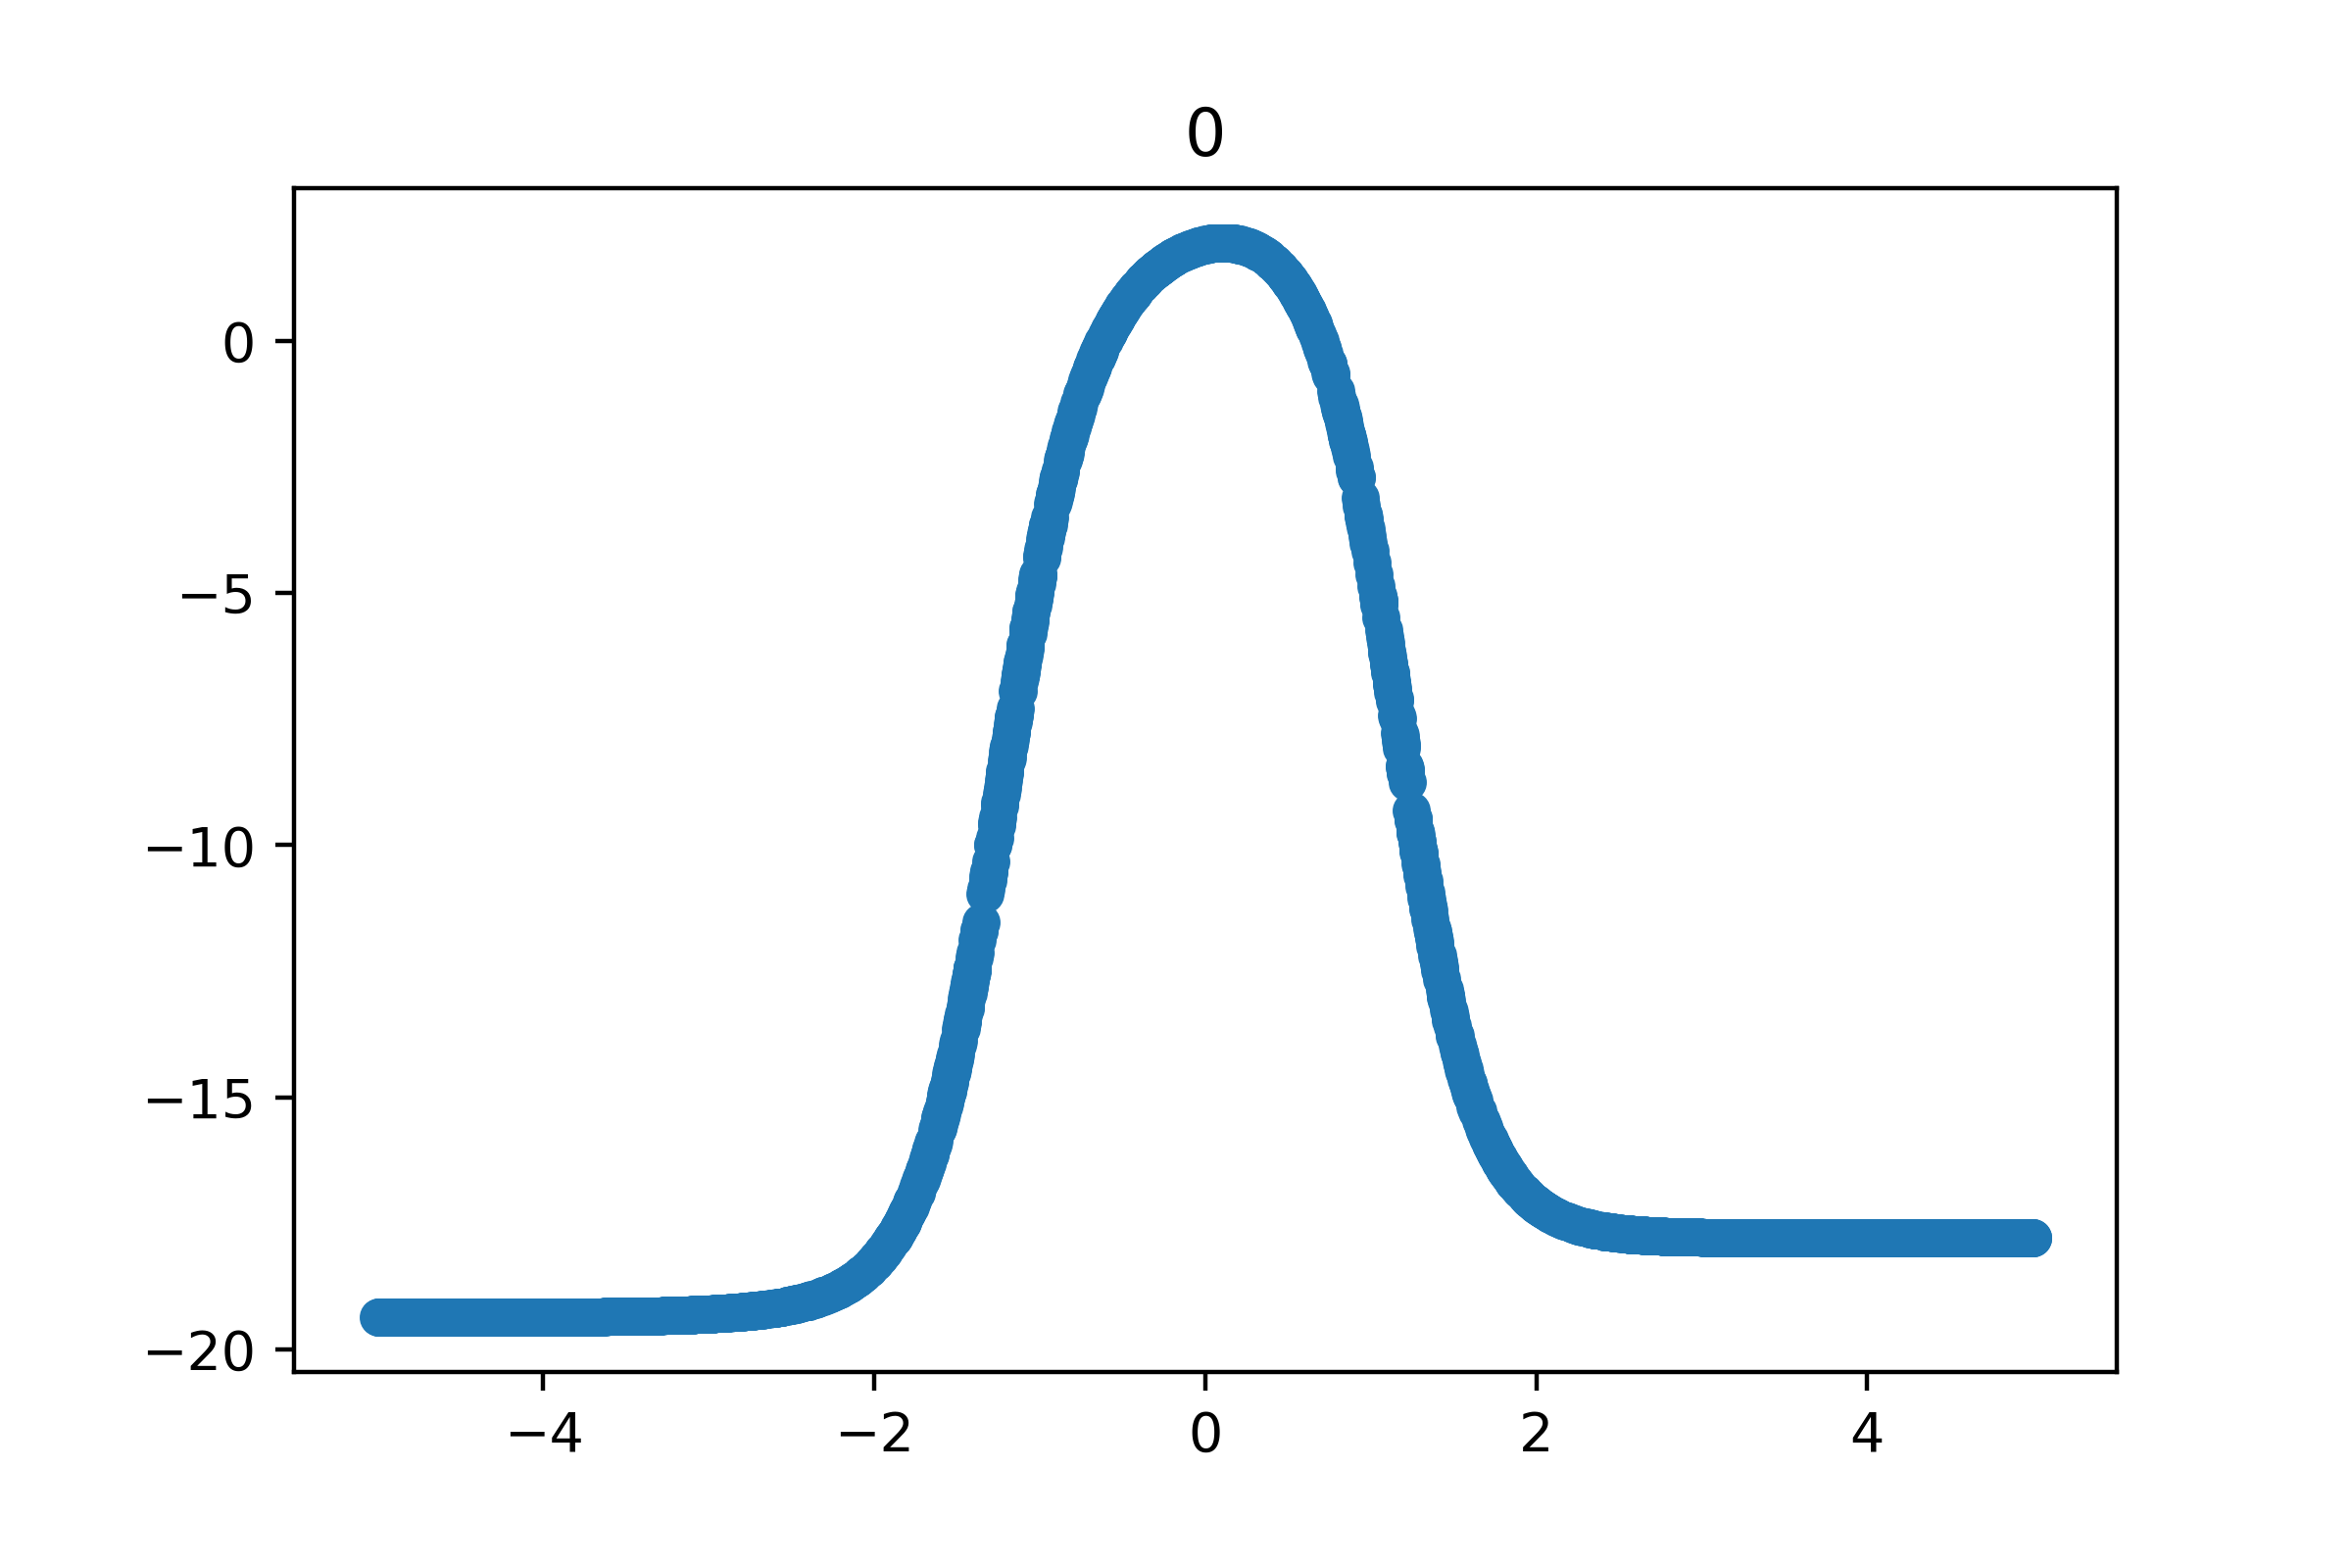
\includegraphics[width=.99\textwidth]{fig/mnl/ci1.png}
%     \end{subfigure}%
%     \begin{subfigure}{.33\textwidth}
%       \centering
%       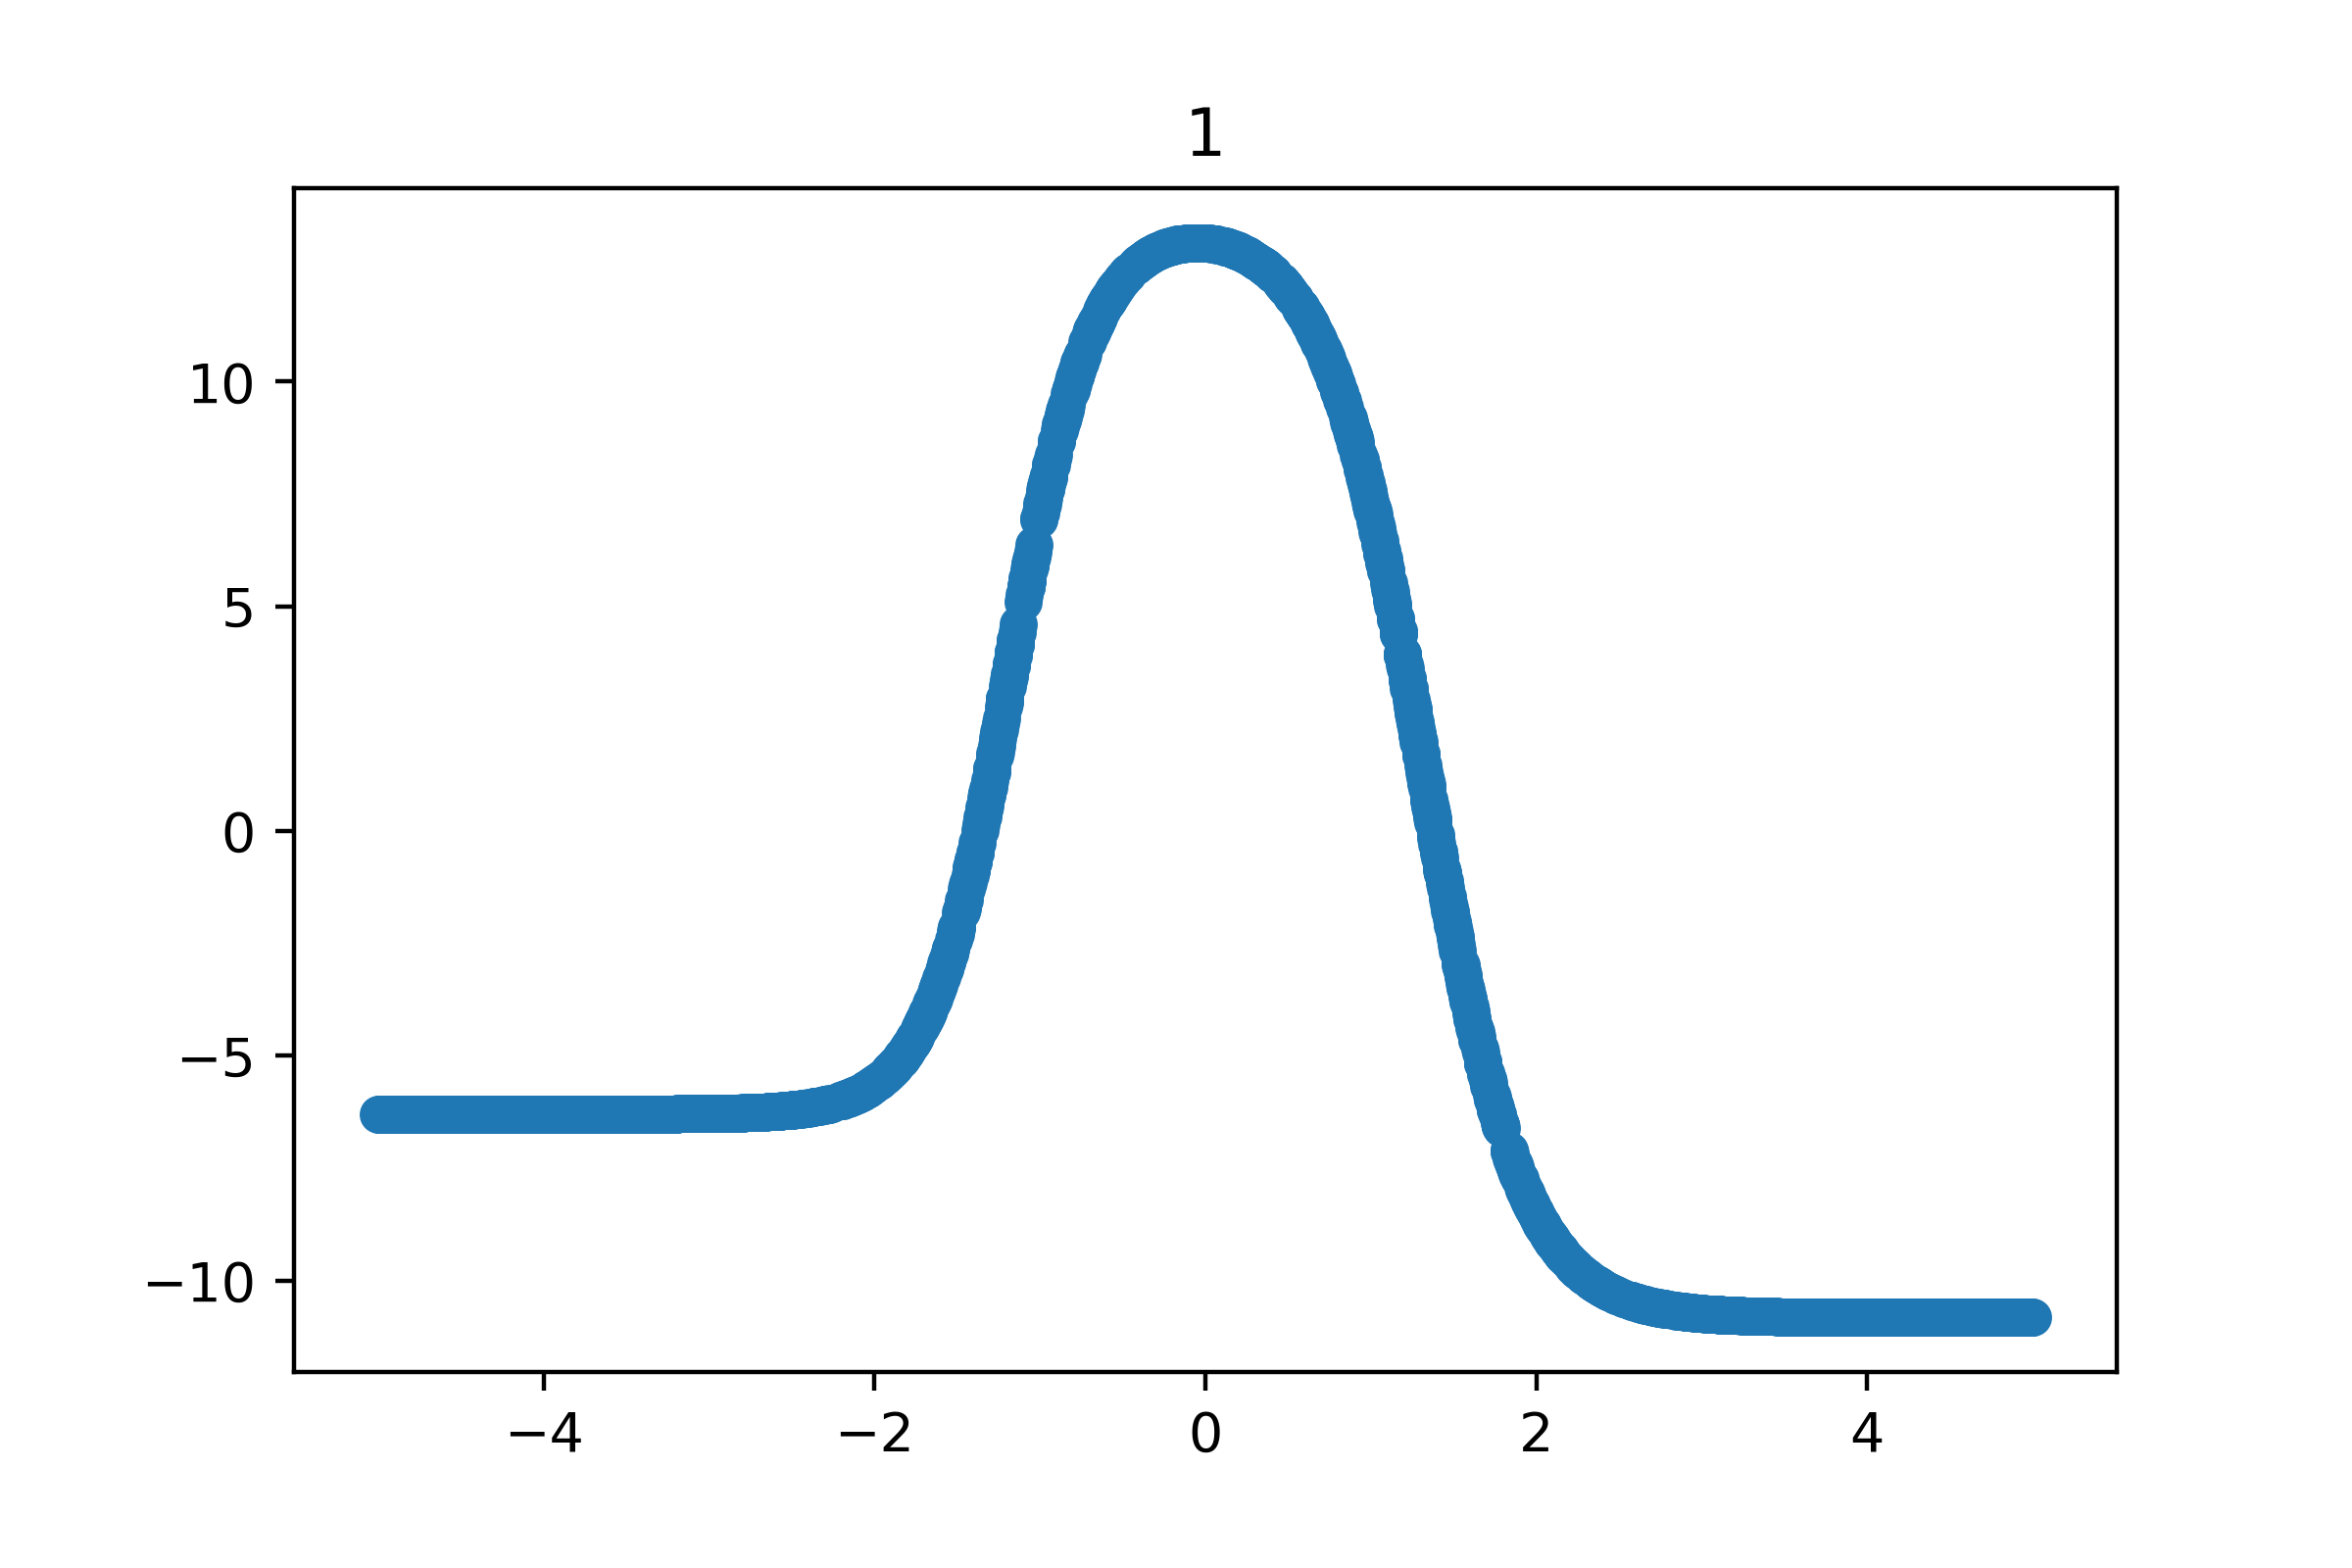
\includegraphics[width=.99\textwidth]{fig/mnl/ci2.png}
%     \end{subfigure}%
%     \begin{subfigure}{.33\textwidth}
%       \centering
%       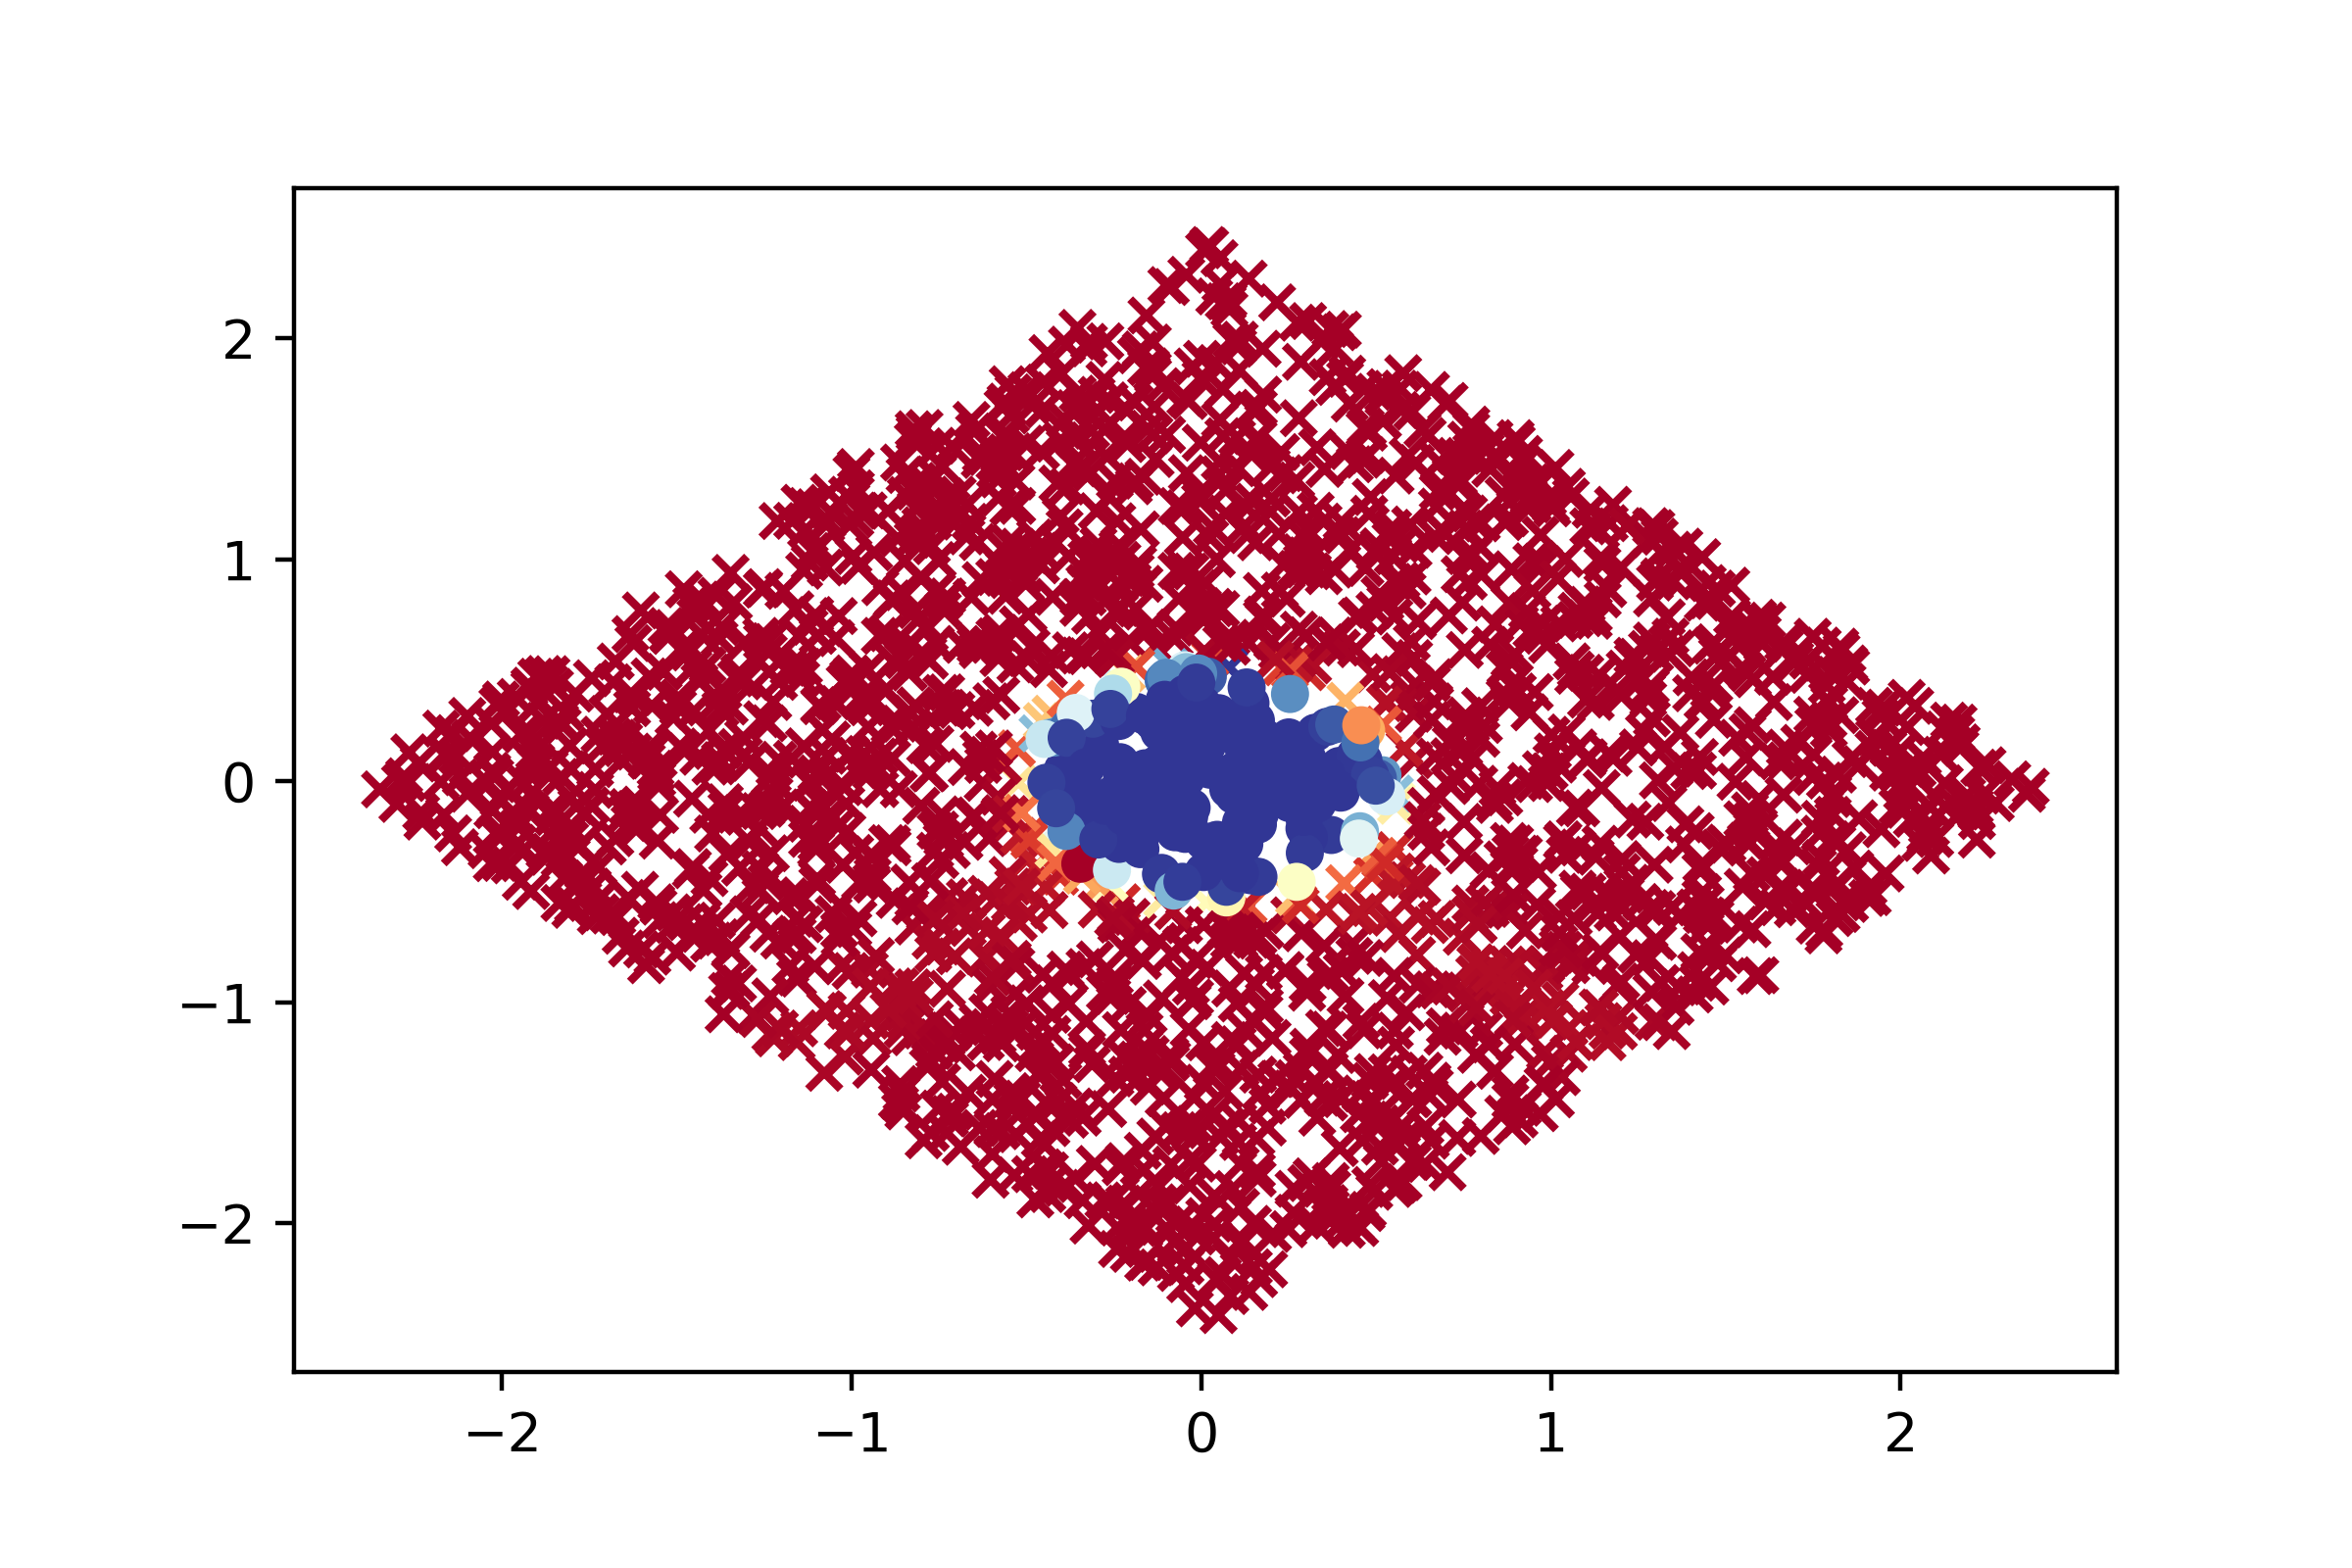
\includegraphics[width=.99\textwidth]{fig/plt/ci.png}
%     \end{subfigure}
%     \caption{TODO}
% \end{figure}


% \begin{figure}
%     \begin{center}
%         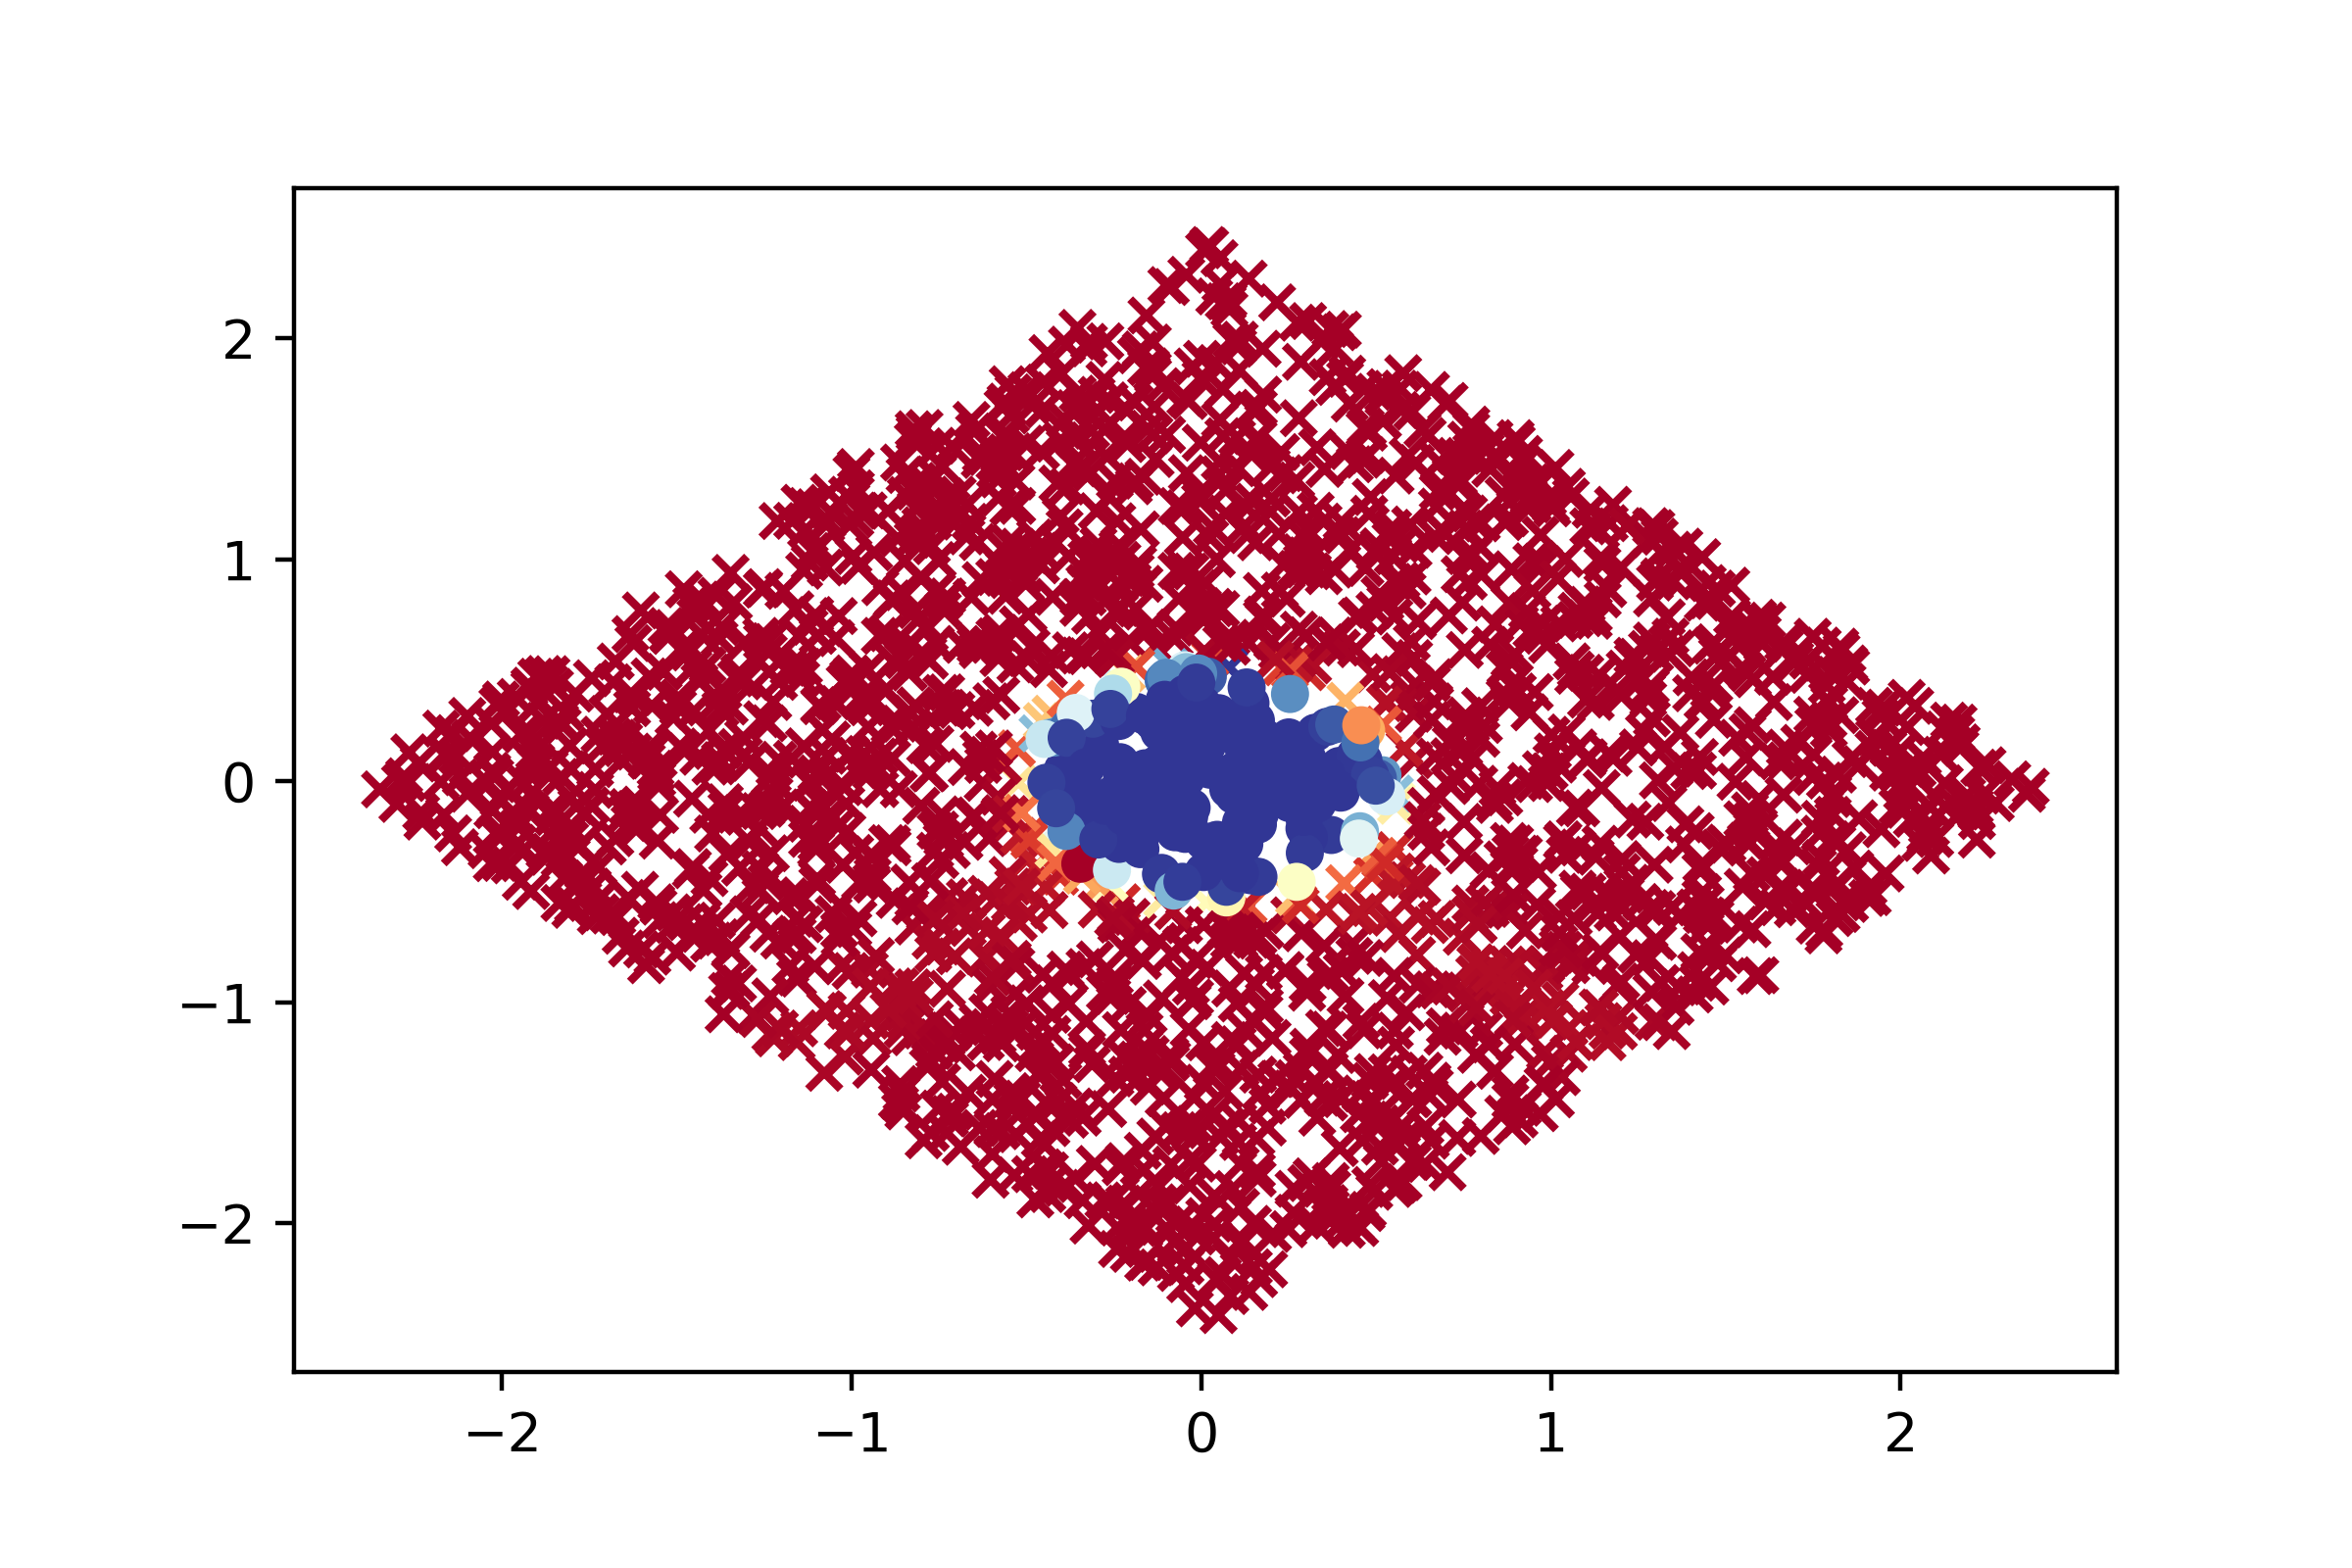
\includegraphics[width=.5\textwidth]{fig/plt/ci.png}
%         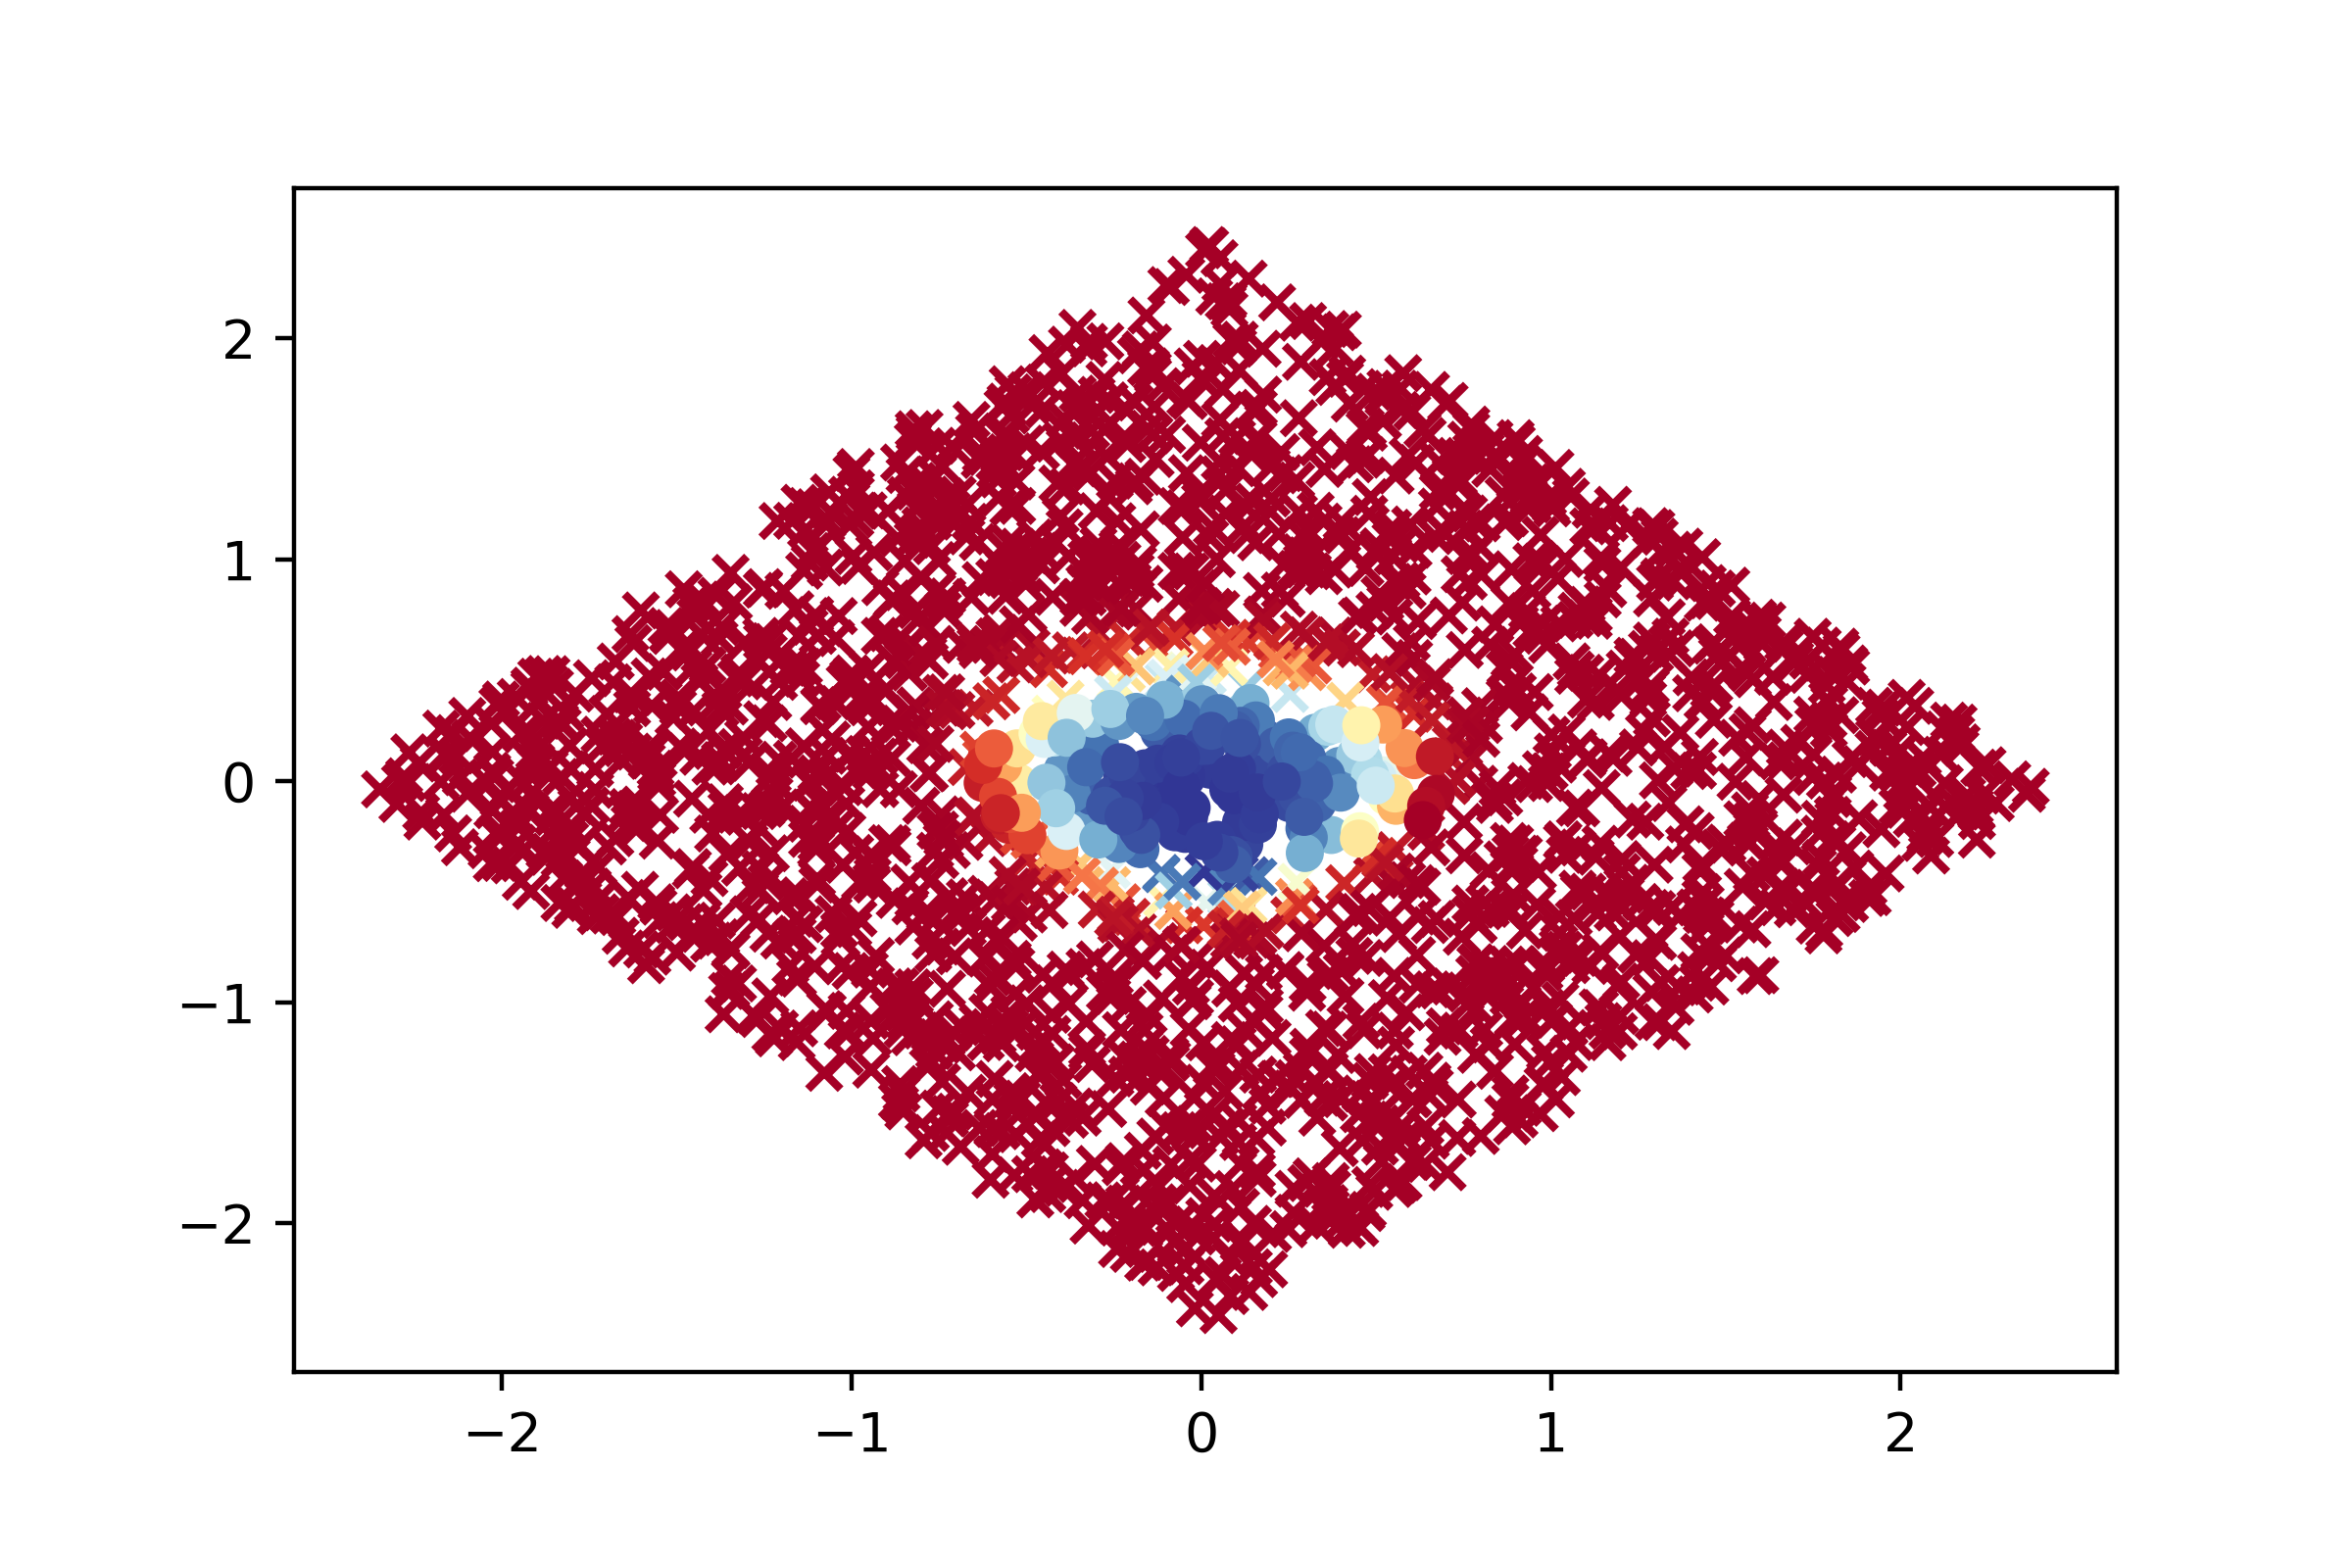
\includegraphics[width=.5\textwidth]{fig/plt/el.png}
%         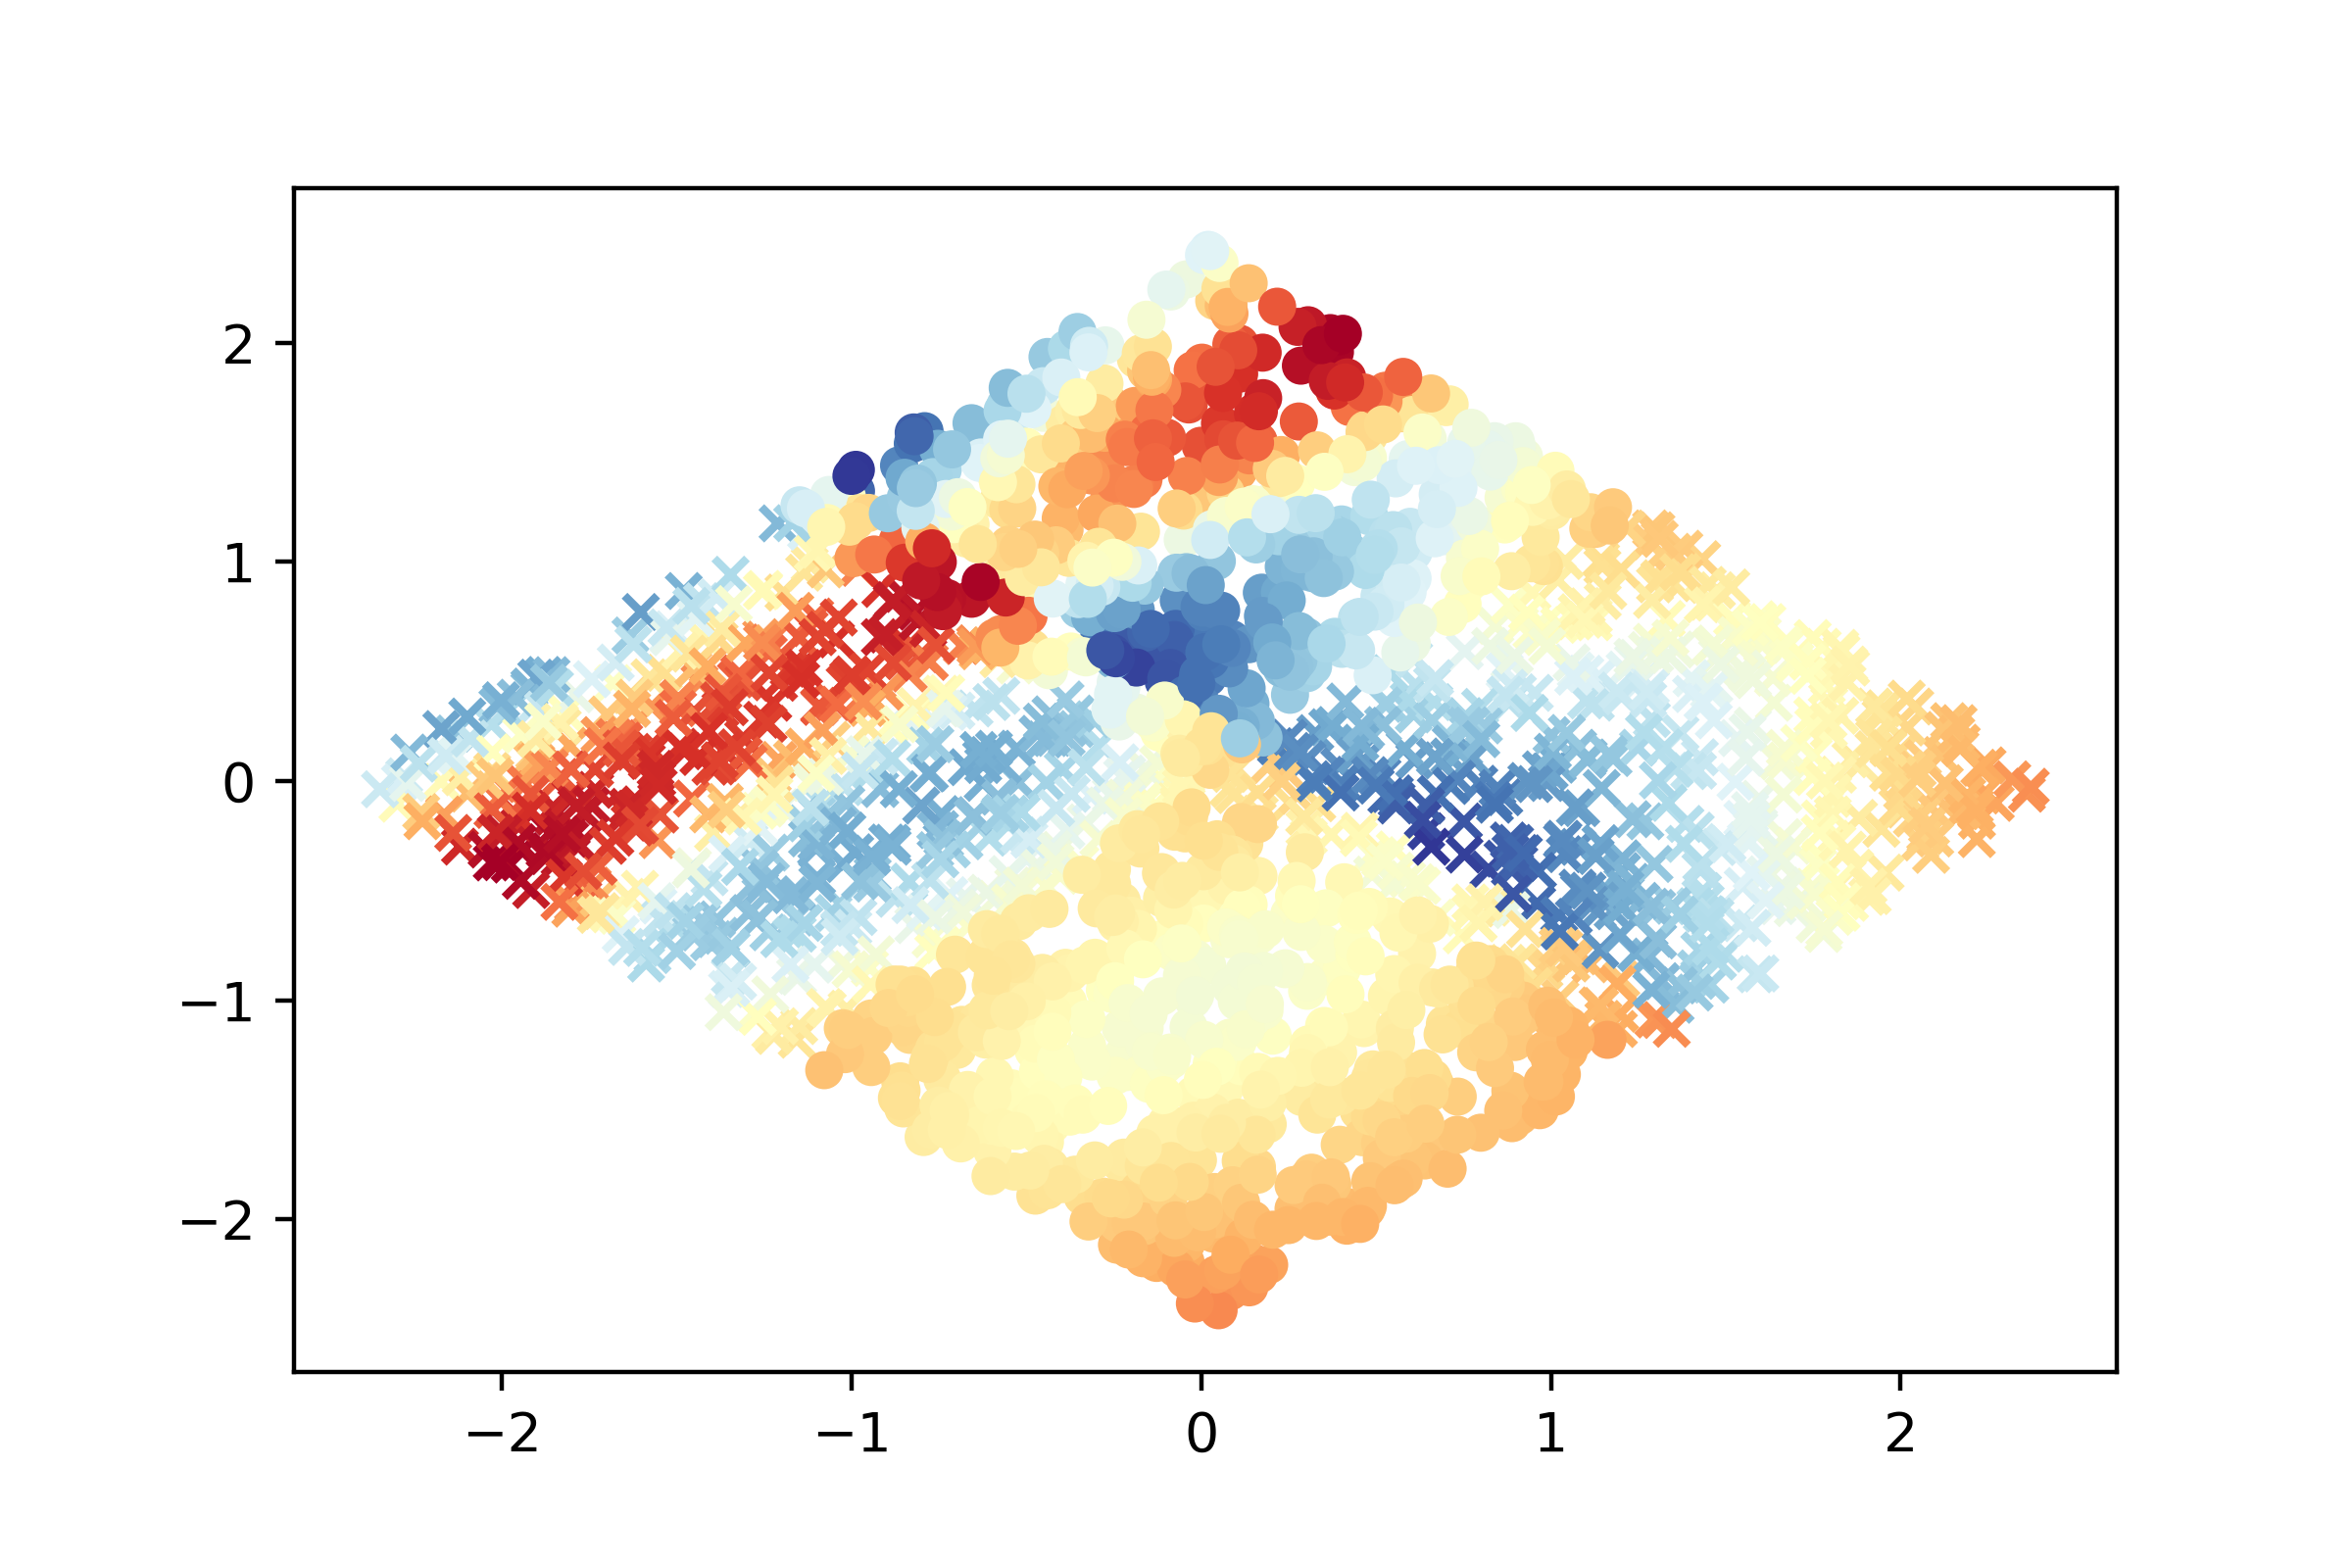
\includegraphics[width=.5\textwidth]{fig/plt/xr.png}
%     \end{center}
%     \caption{4 figures}
% \end{figure}




% \begin{figure}
%     \centering
%     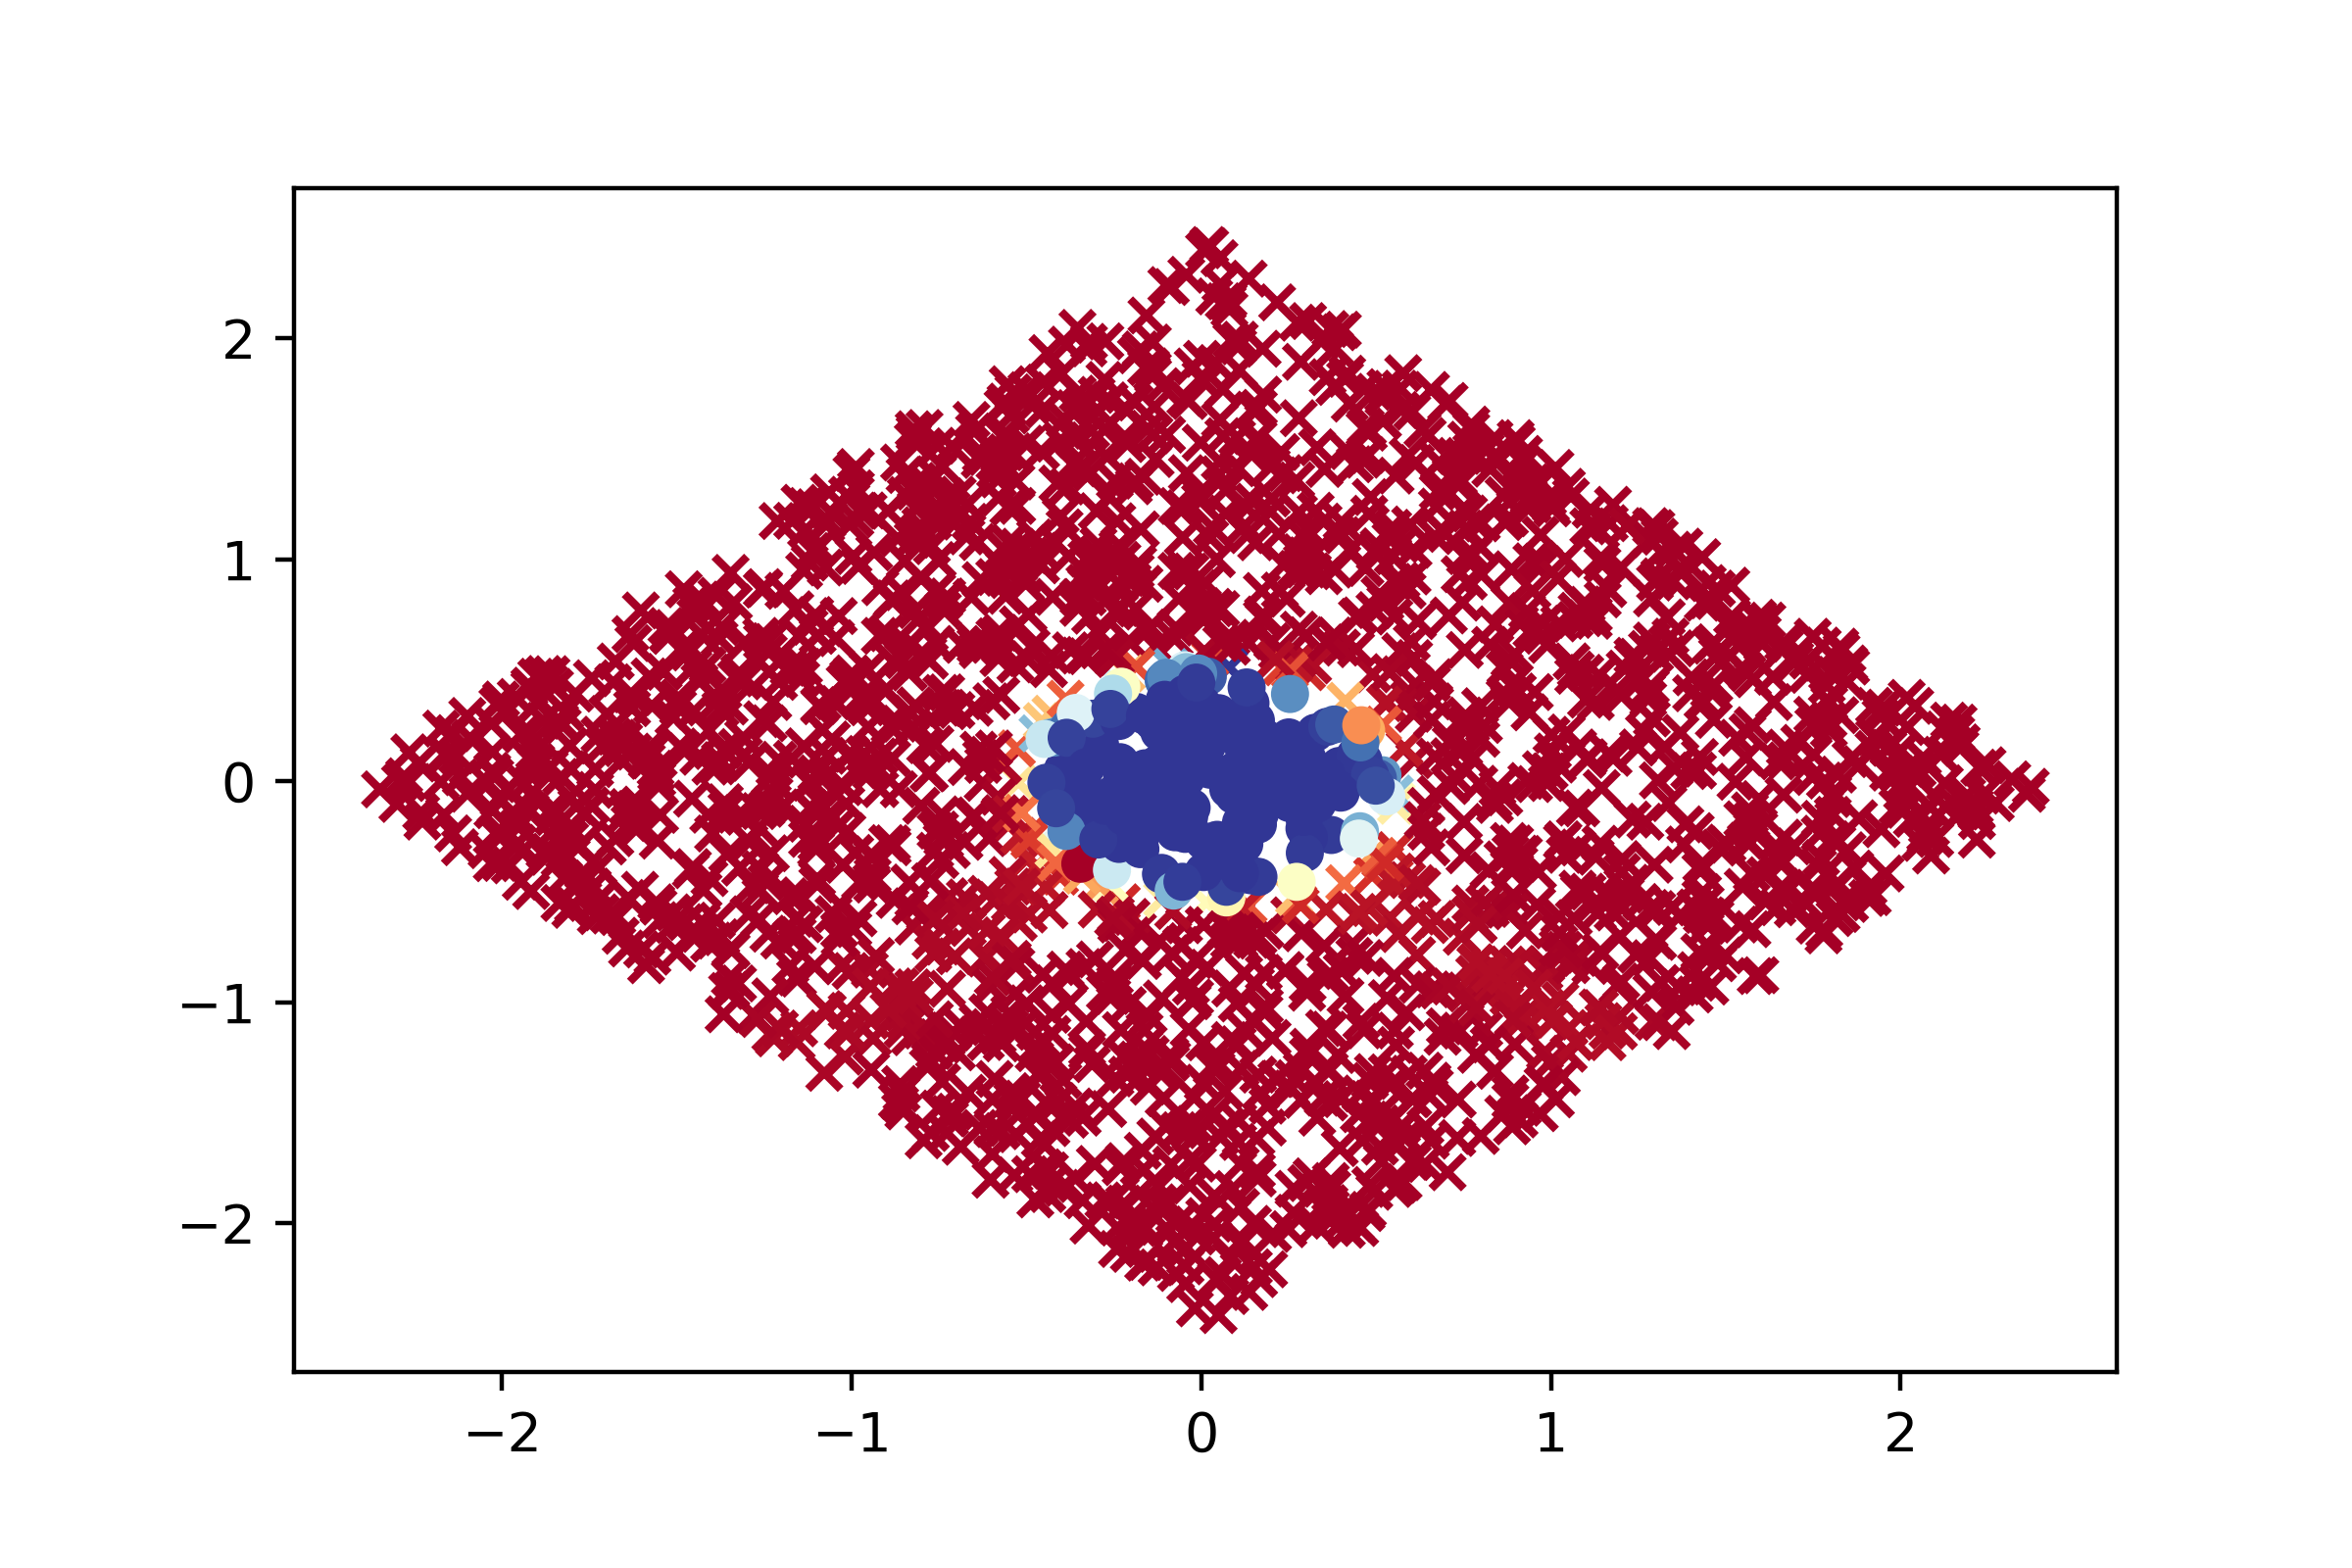
\includegraphics[width=0.65\textwidth]{fig/plt/ci.png}
%     \caption{Network predictions for the circle dataset. The architecture does a good job of isolating the center region.}
% \end{figure}

% \begin{figure}
%     \centering
%     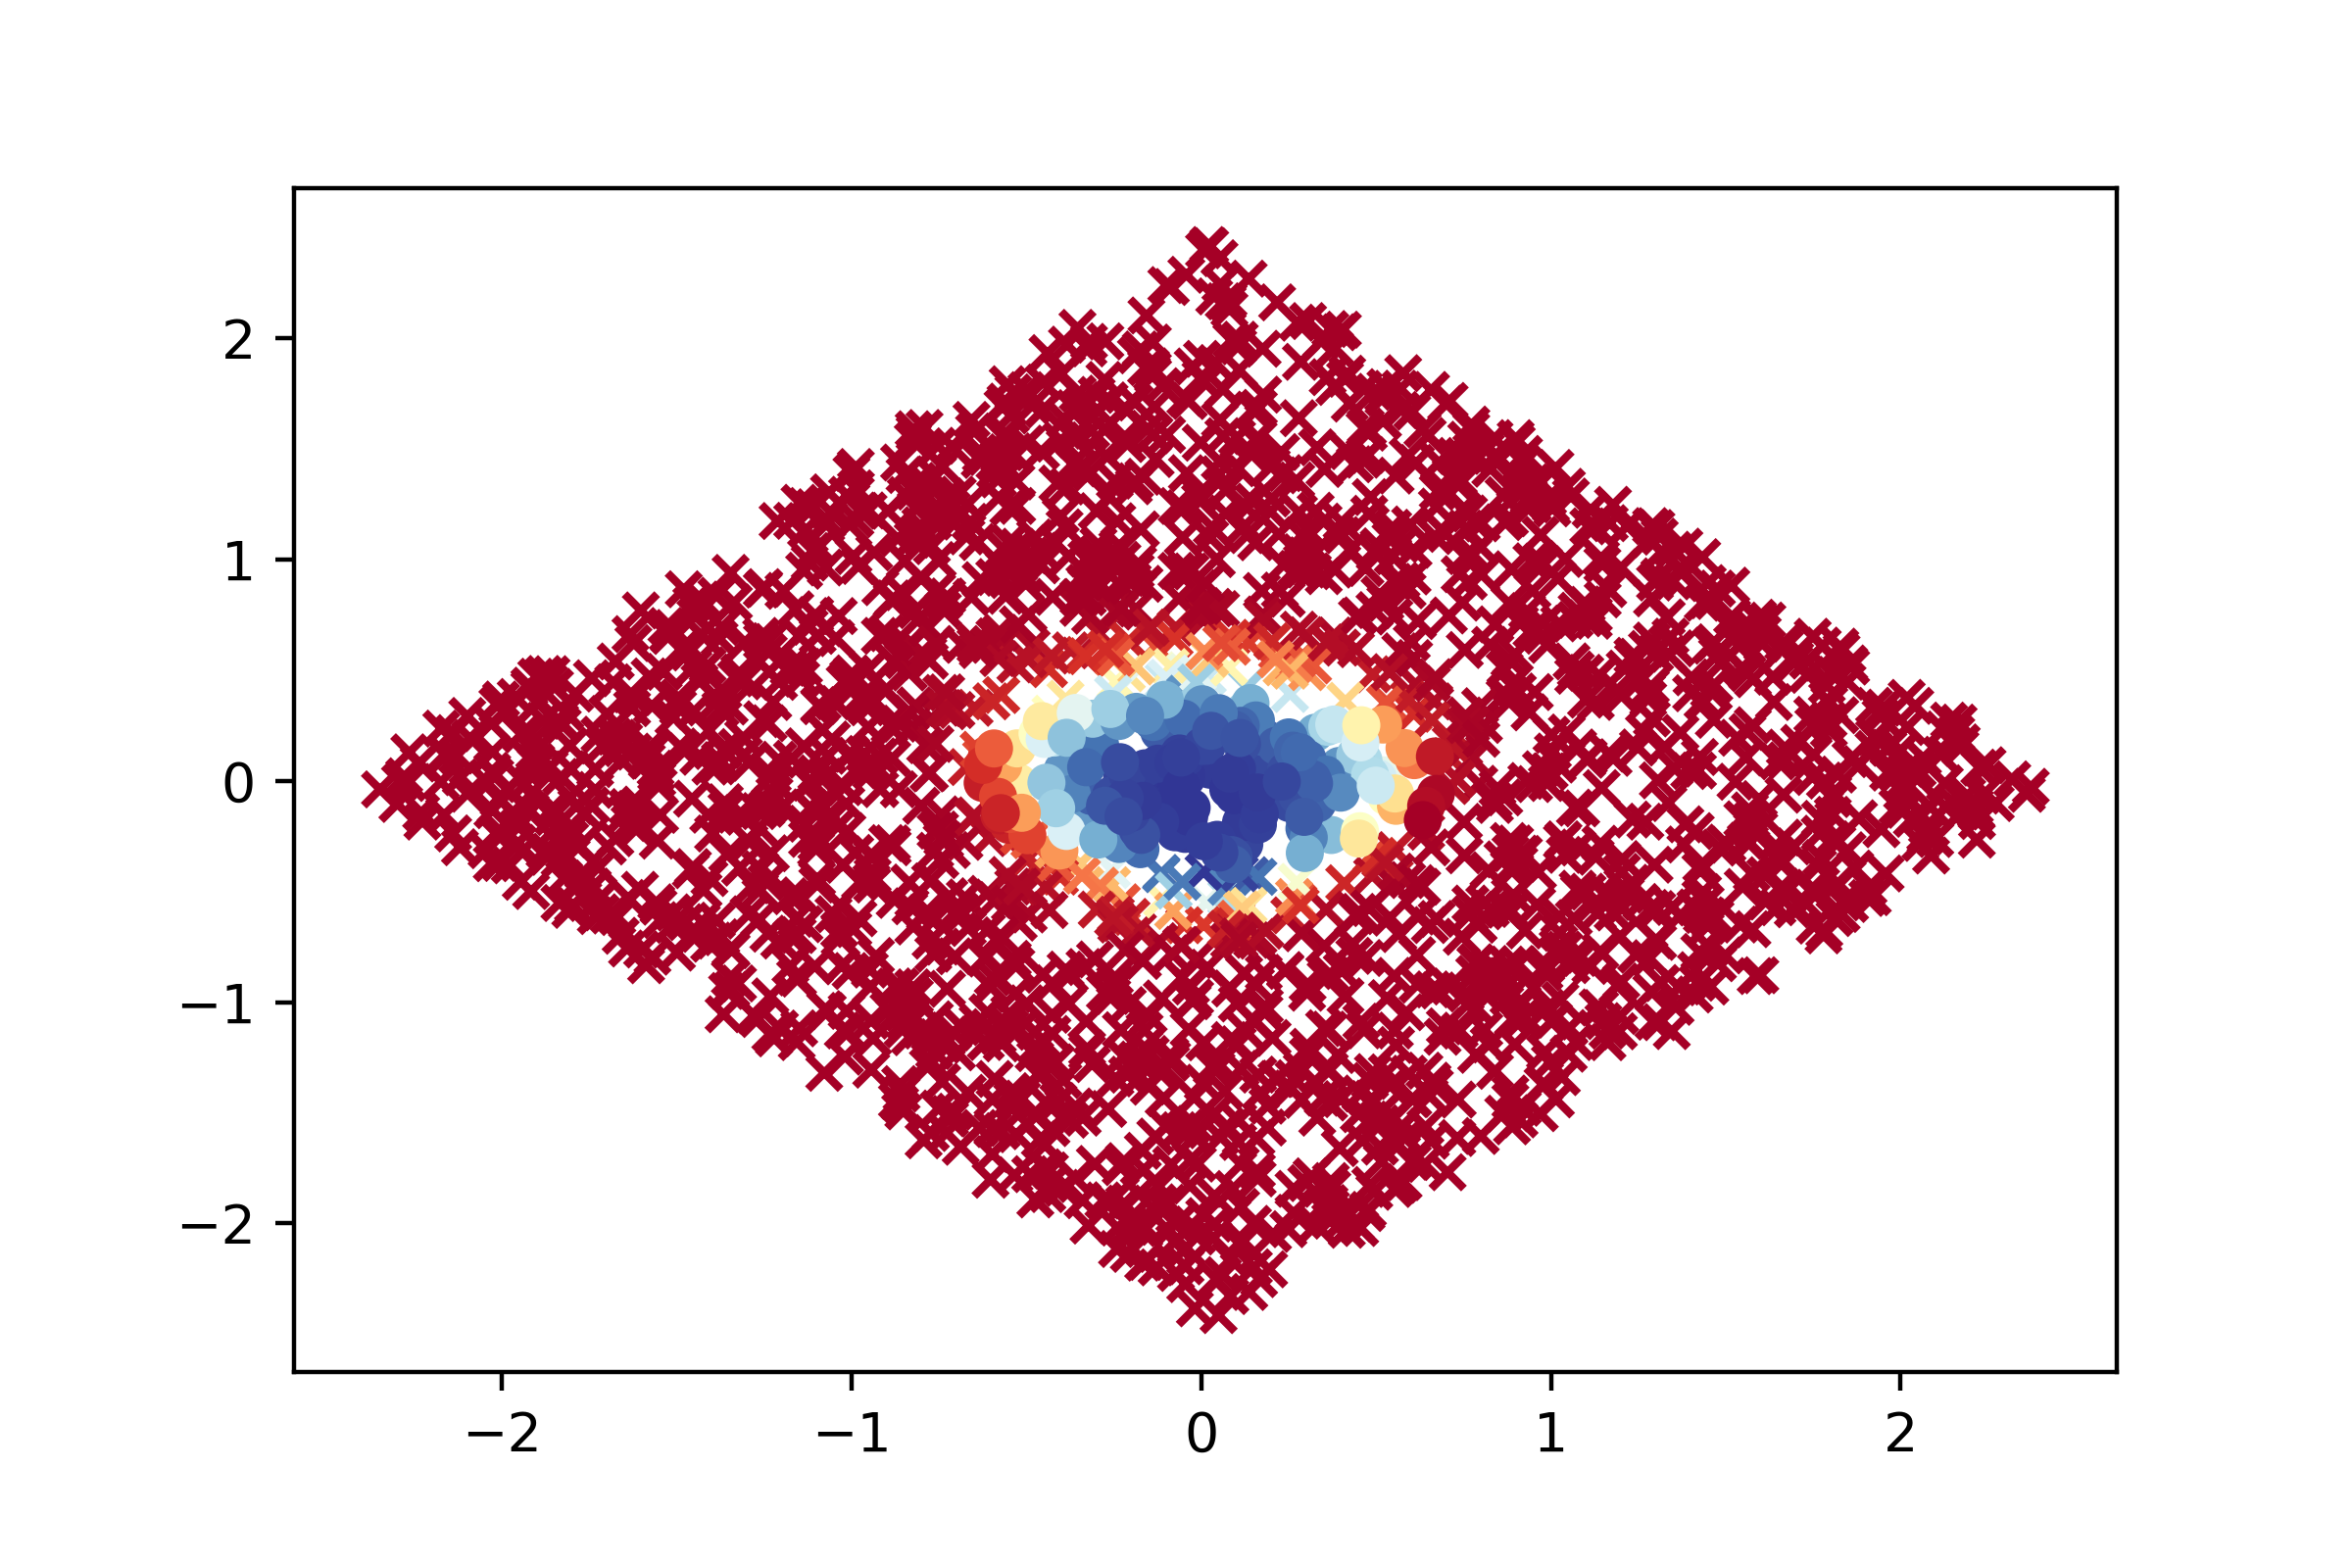
\includegraphics[width=0.65\textwidth]{fig/plt/el.png}
%     \caption{Network predictions for the ellipse dataset. The architecture captures a circular region in the center, but struggles on the elliptical section, represented by the yellow ring around the center predictions.}
% \end{figure}

% \begin{figure}
%     \centering
%     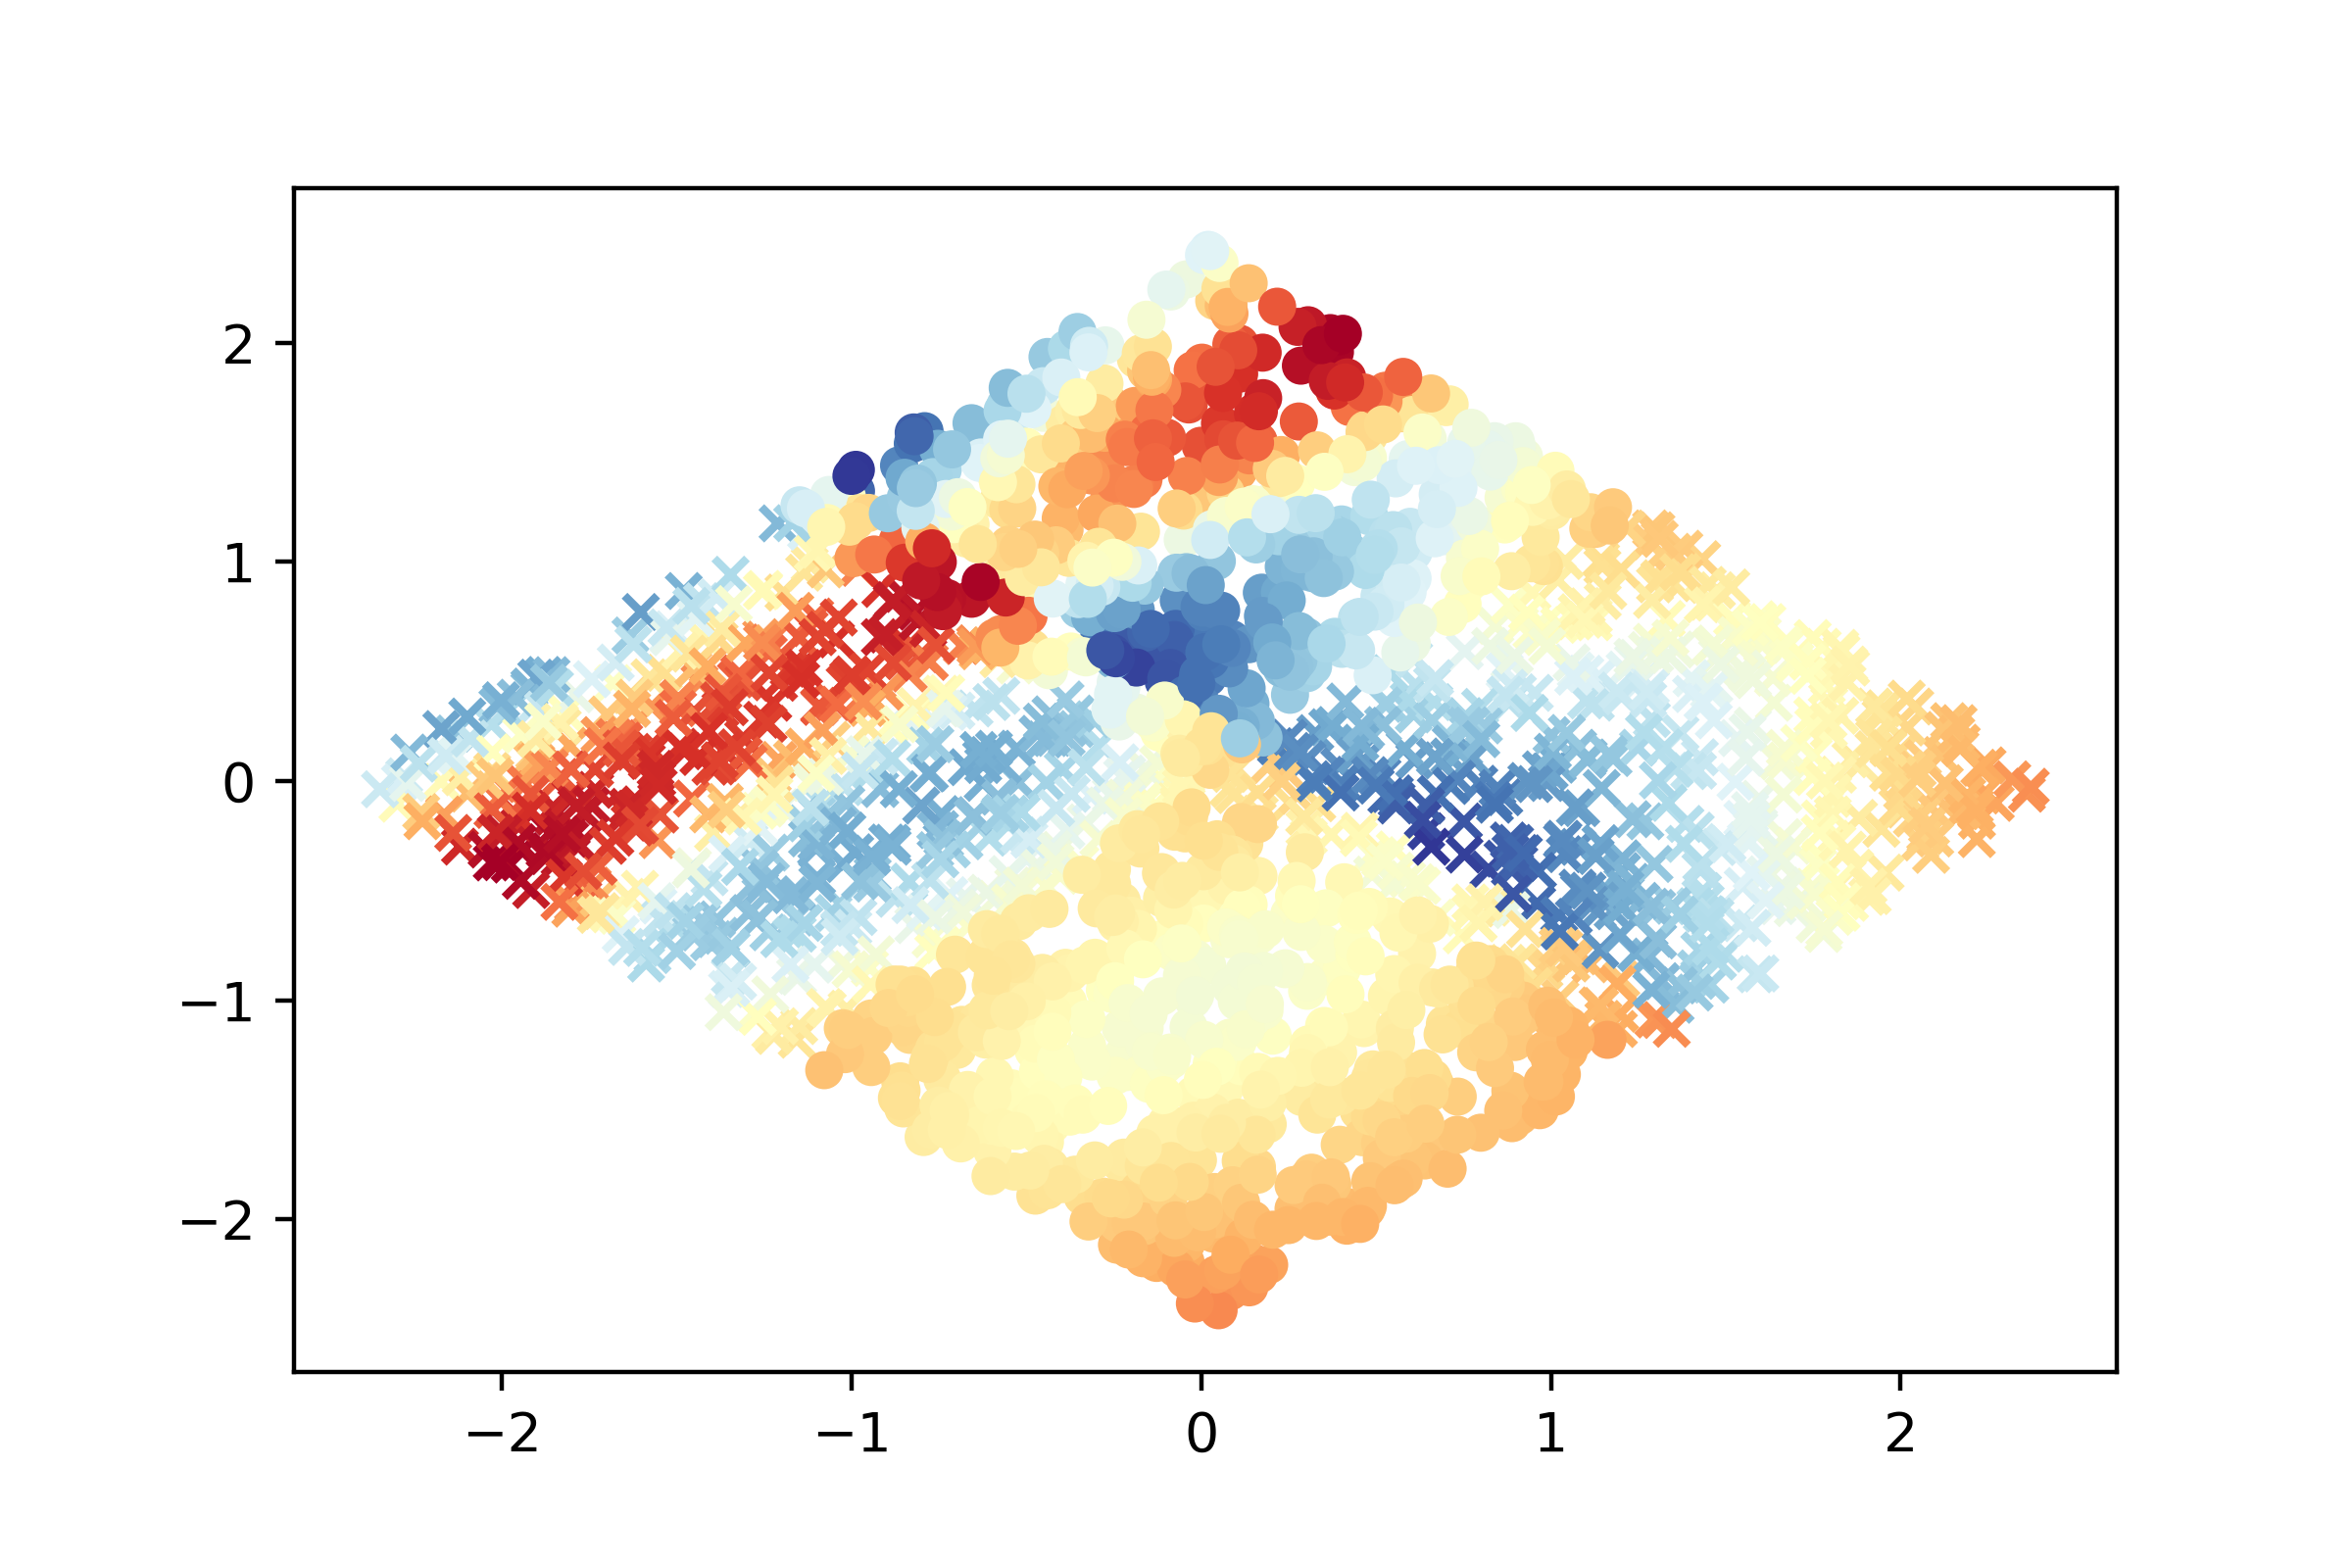
\includegraphics[width=0.65\textwidth]{fig/plt/xr.png}
%     \caption{Network predictions for the XOR dataset. The architecture fails to arrive at a reasonable prediction for the dataset.}
% \end{figure}





% \begin{longtable}[]{@{}lc@{}}

%     \toprule
%     Dataset & PCA Plot%
%     \tabularnewline
%     \midrule
%     \endhead

%     Circle &
%     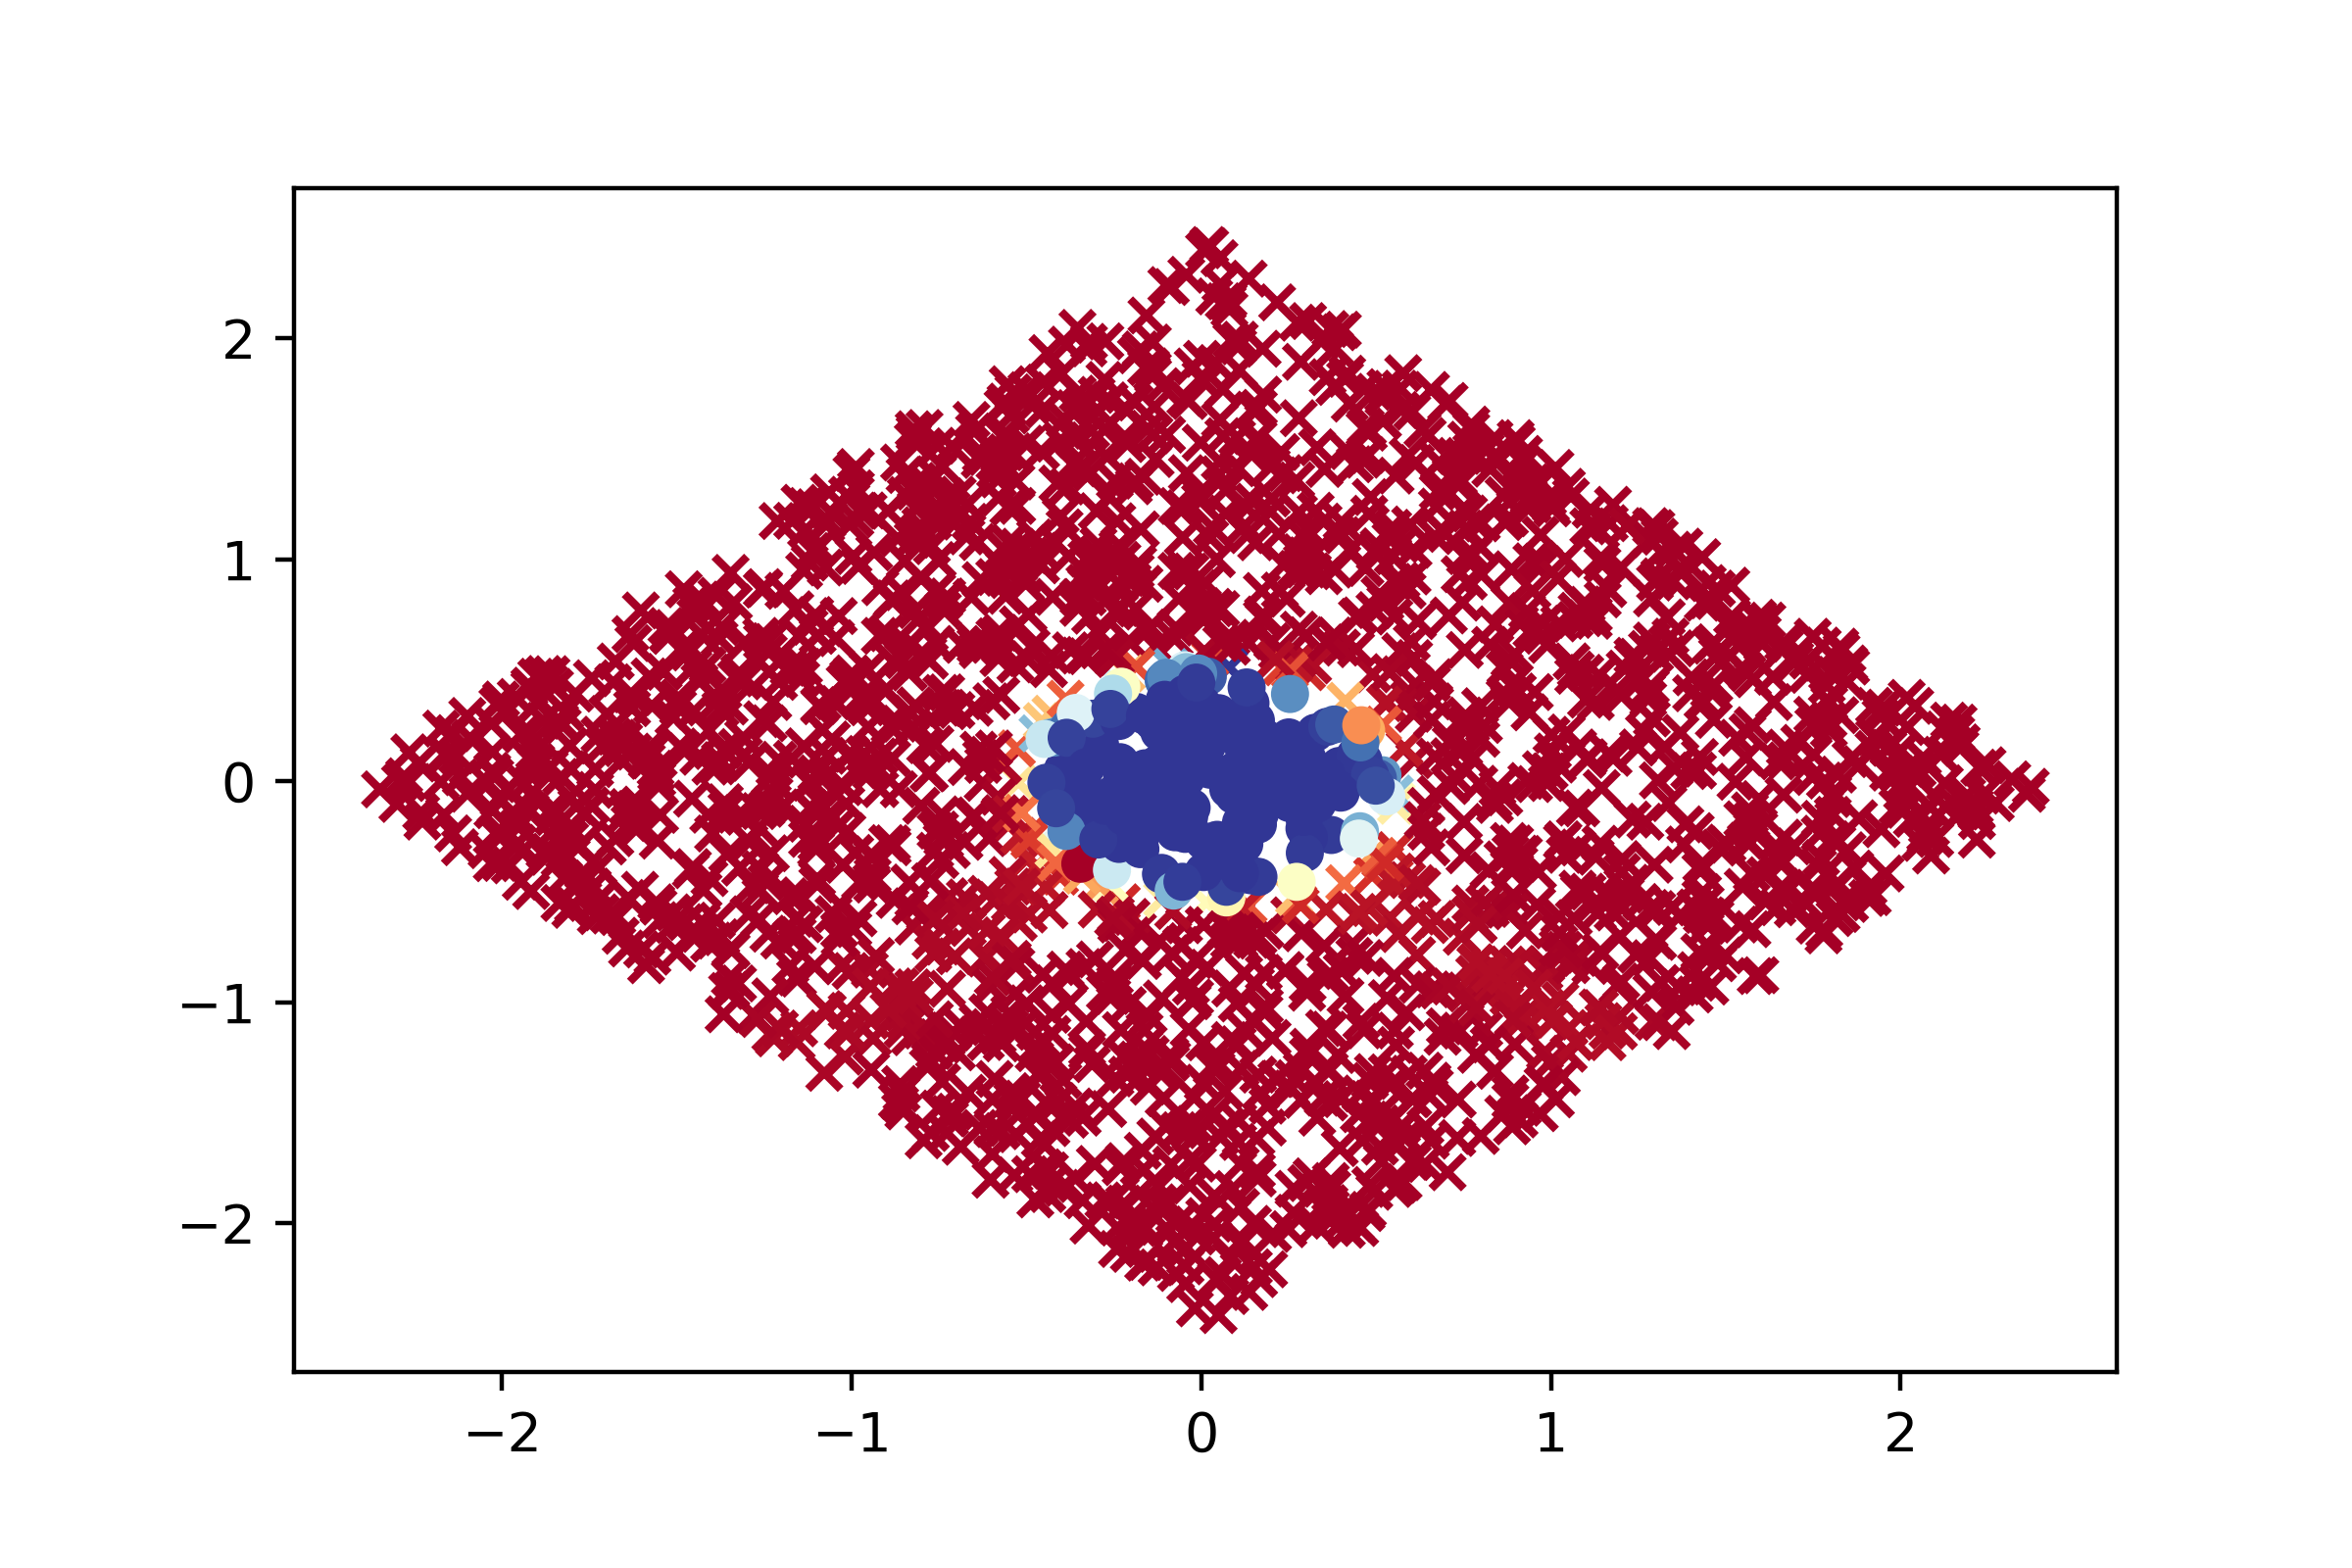
\includegraphics[width=0.80\textwidth]{fig/plt/ci.png} \tabularnewline
    
%     Ellipse & 
%     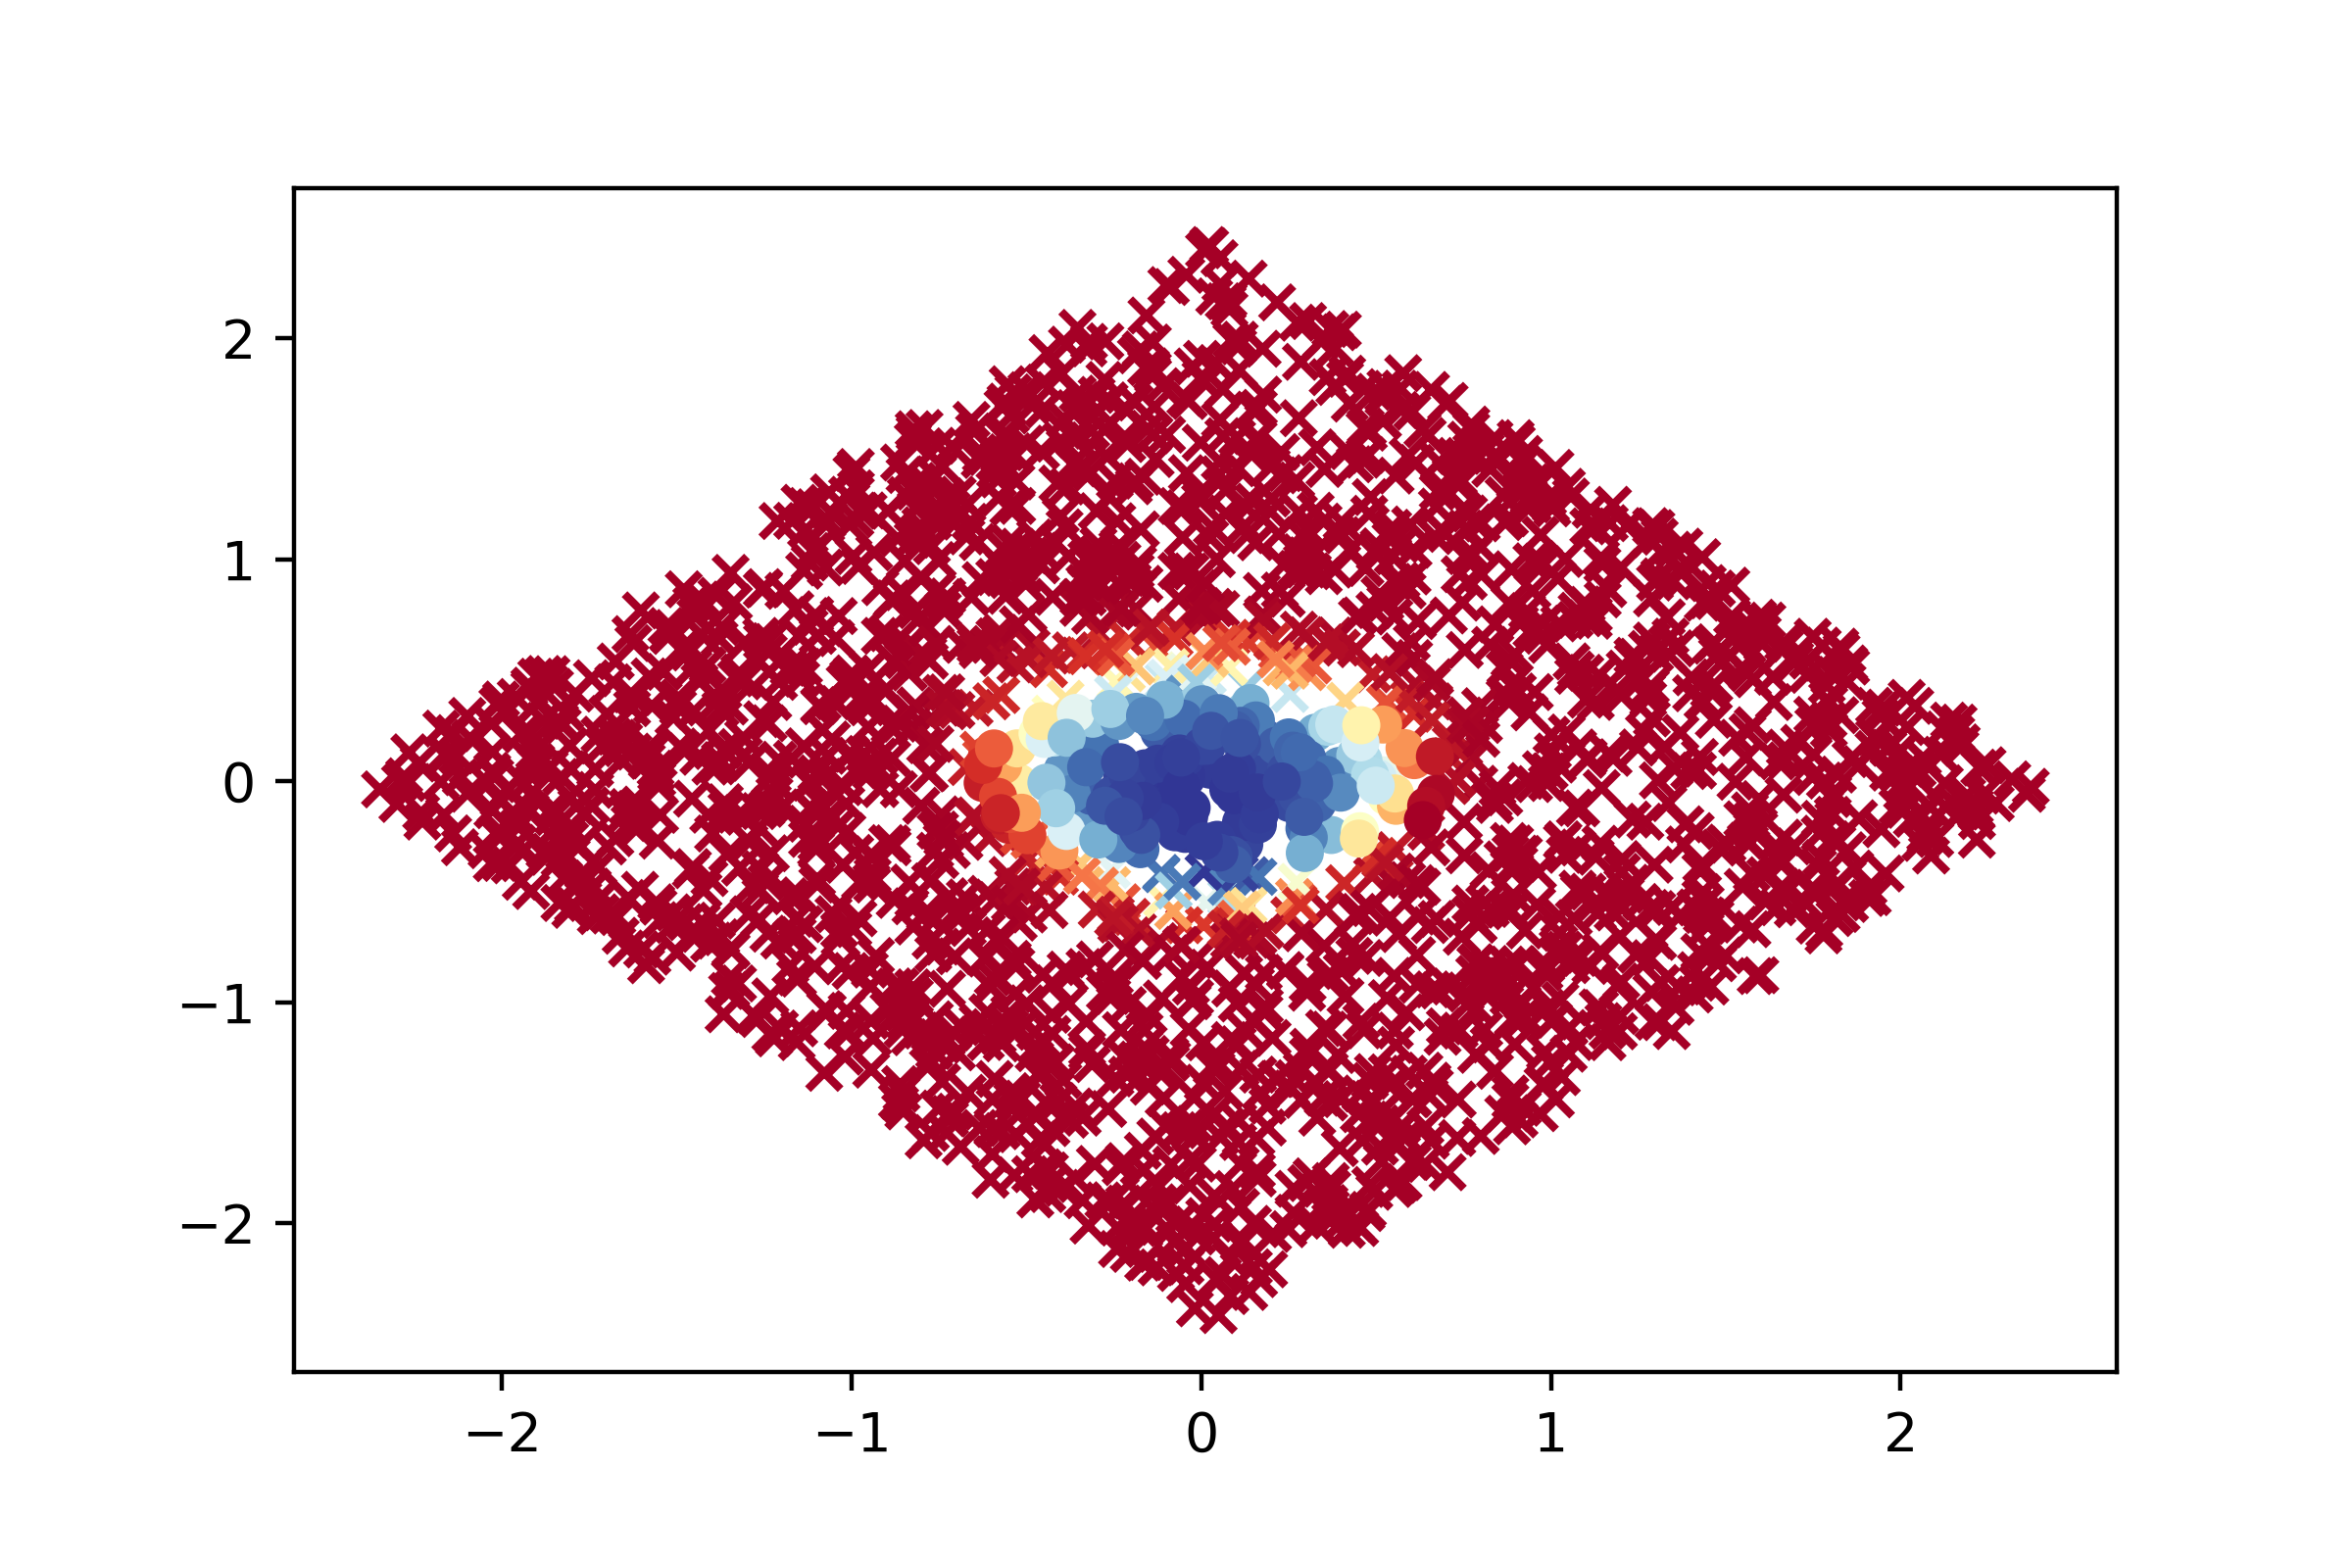
\includegraphics[width=0.80\textwidth]{fig/plt/el.png} \tabularnewline
    
%     XOR & 
%     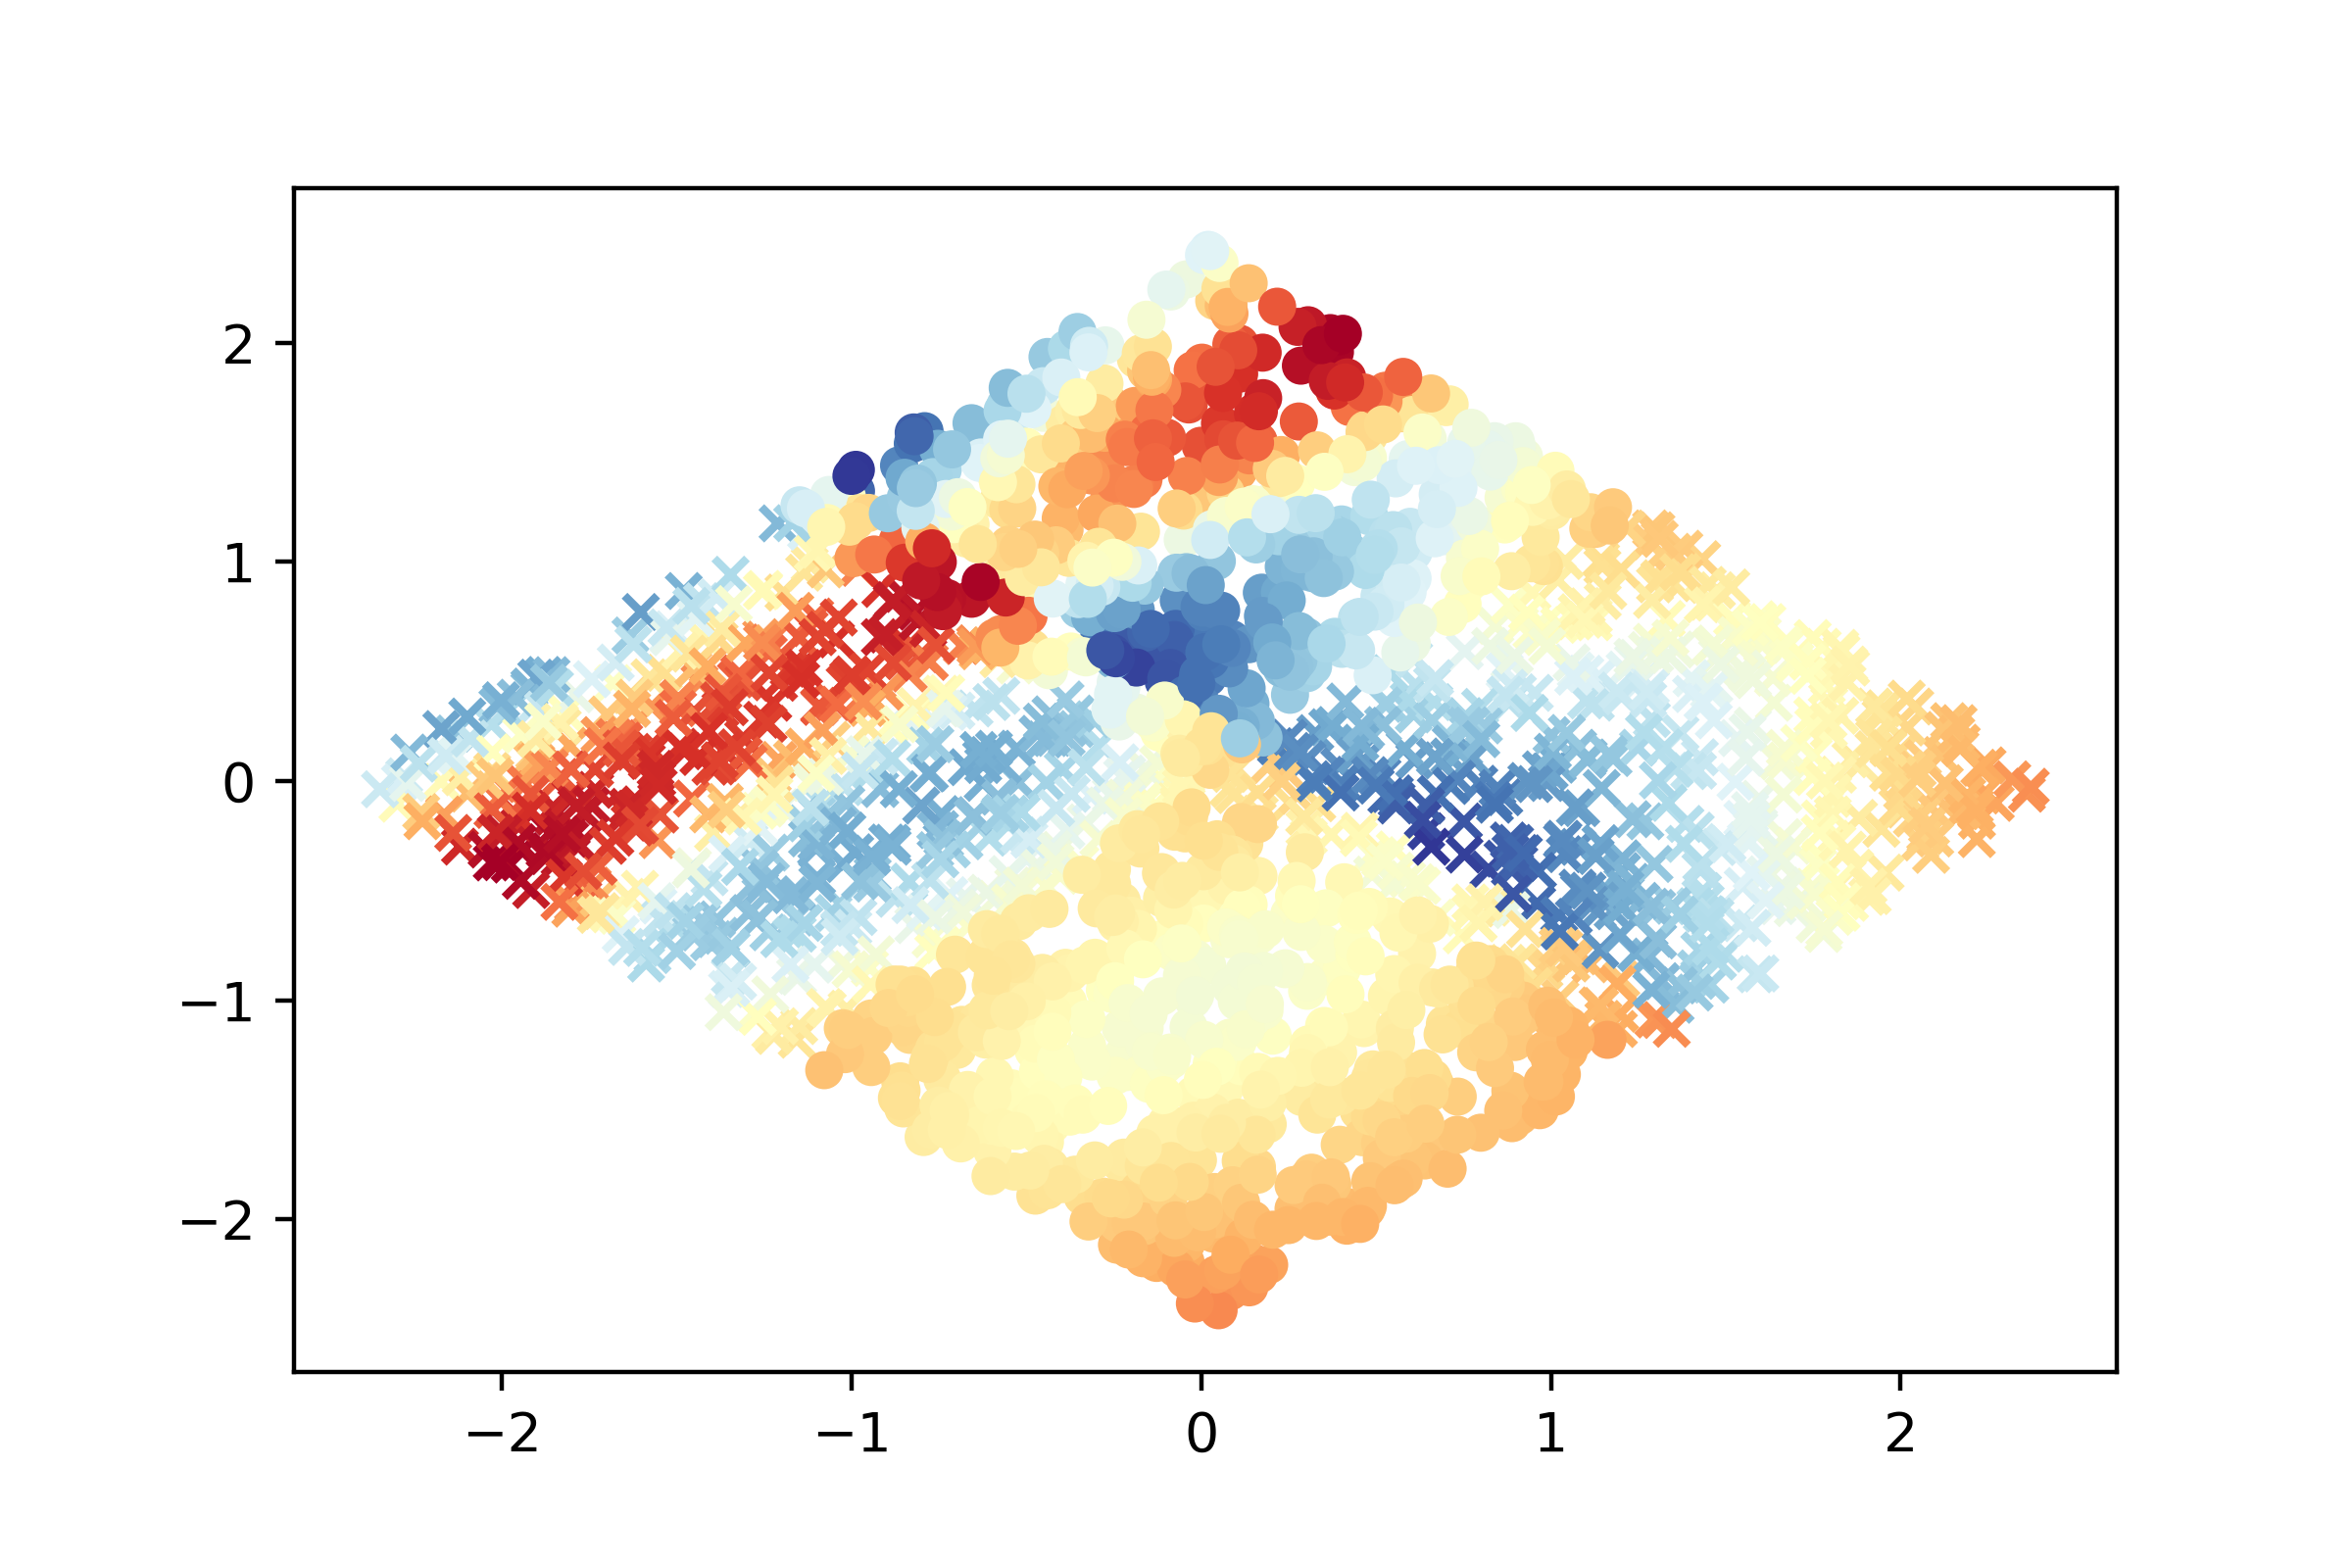
\includegraphics[width=0.80\textwidth]{fig/plt/xr.png} \tabularnewline

%     \bottomrule
    
%     \caption{Two-dimensional principle components plot representing the dataset. X's are true negatives and O's are true positives. Colors represent the network prediction, with blue being positive, red being negative, and yellow being neutral.}

% \end{longtable}


% \begin{longtable}[]{@{}lcc@{}}

%     \toprule
%     Dataset & Marginal 1 & Marginal 2%
%     \tabularnewline
%     \midrule
%     \endhead

%     Circle &
%     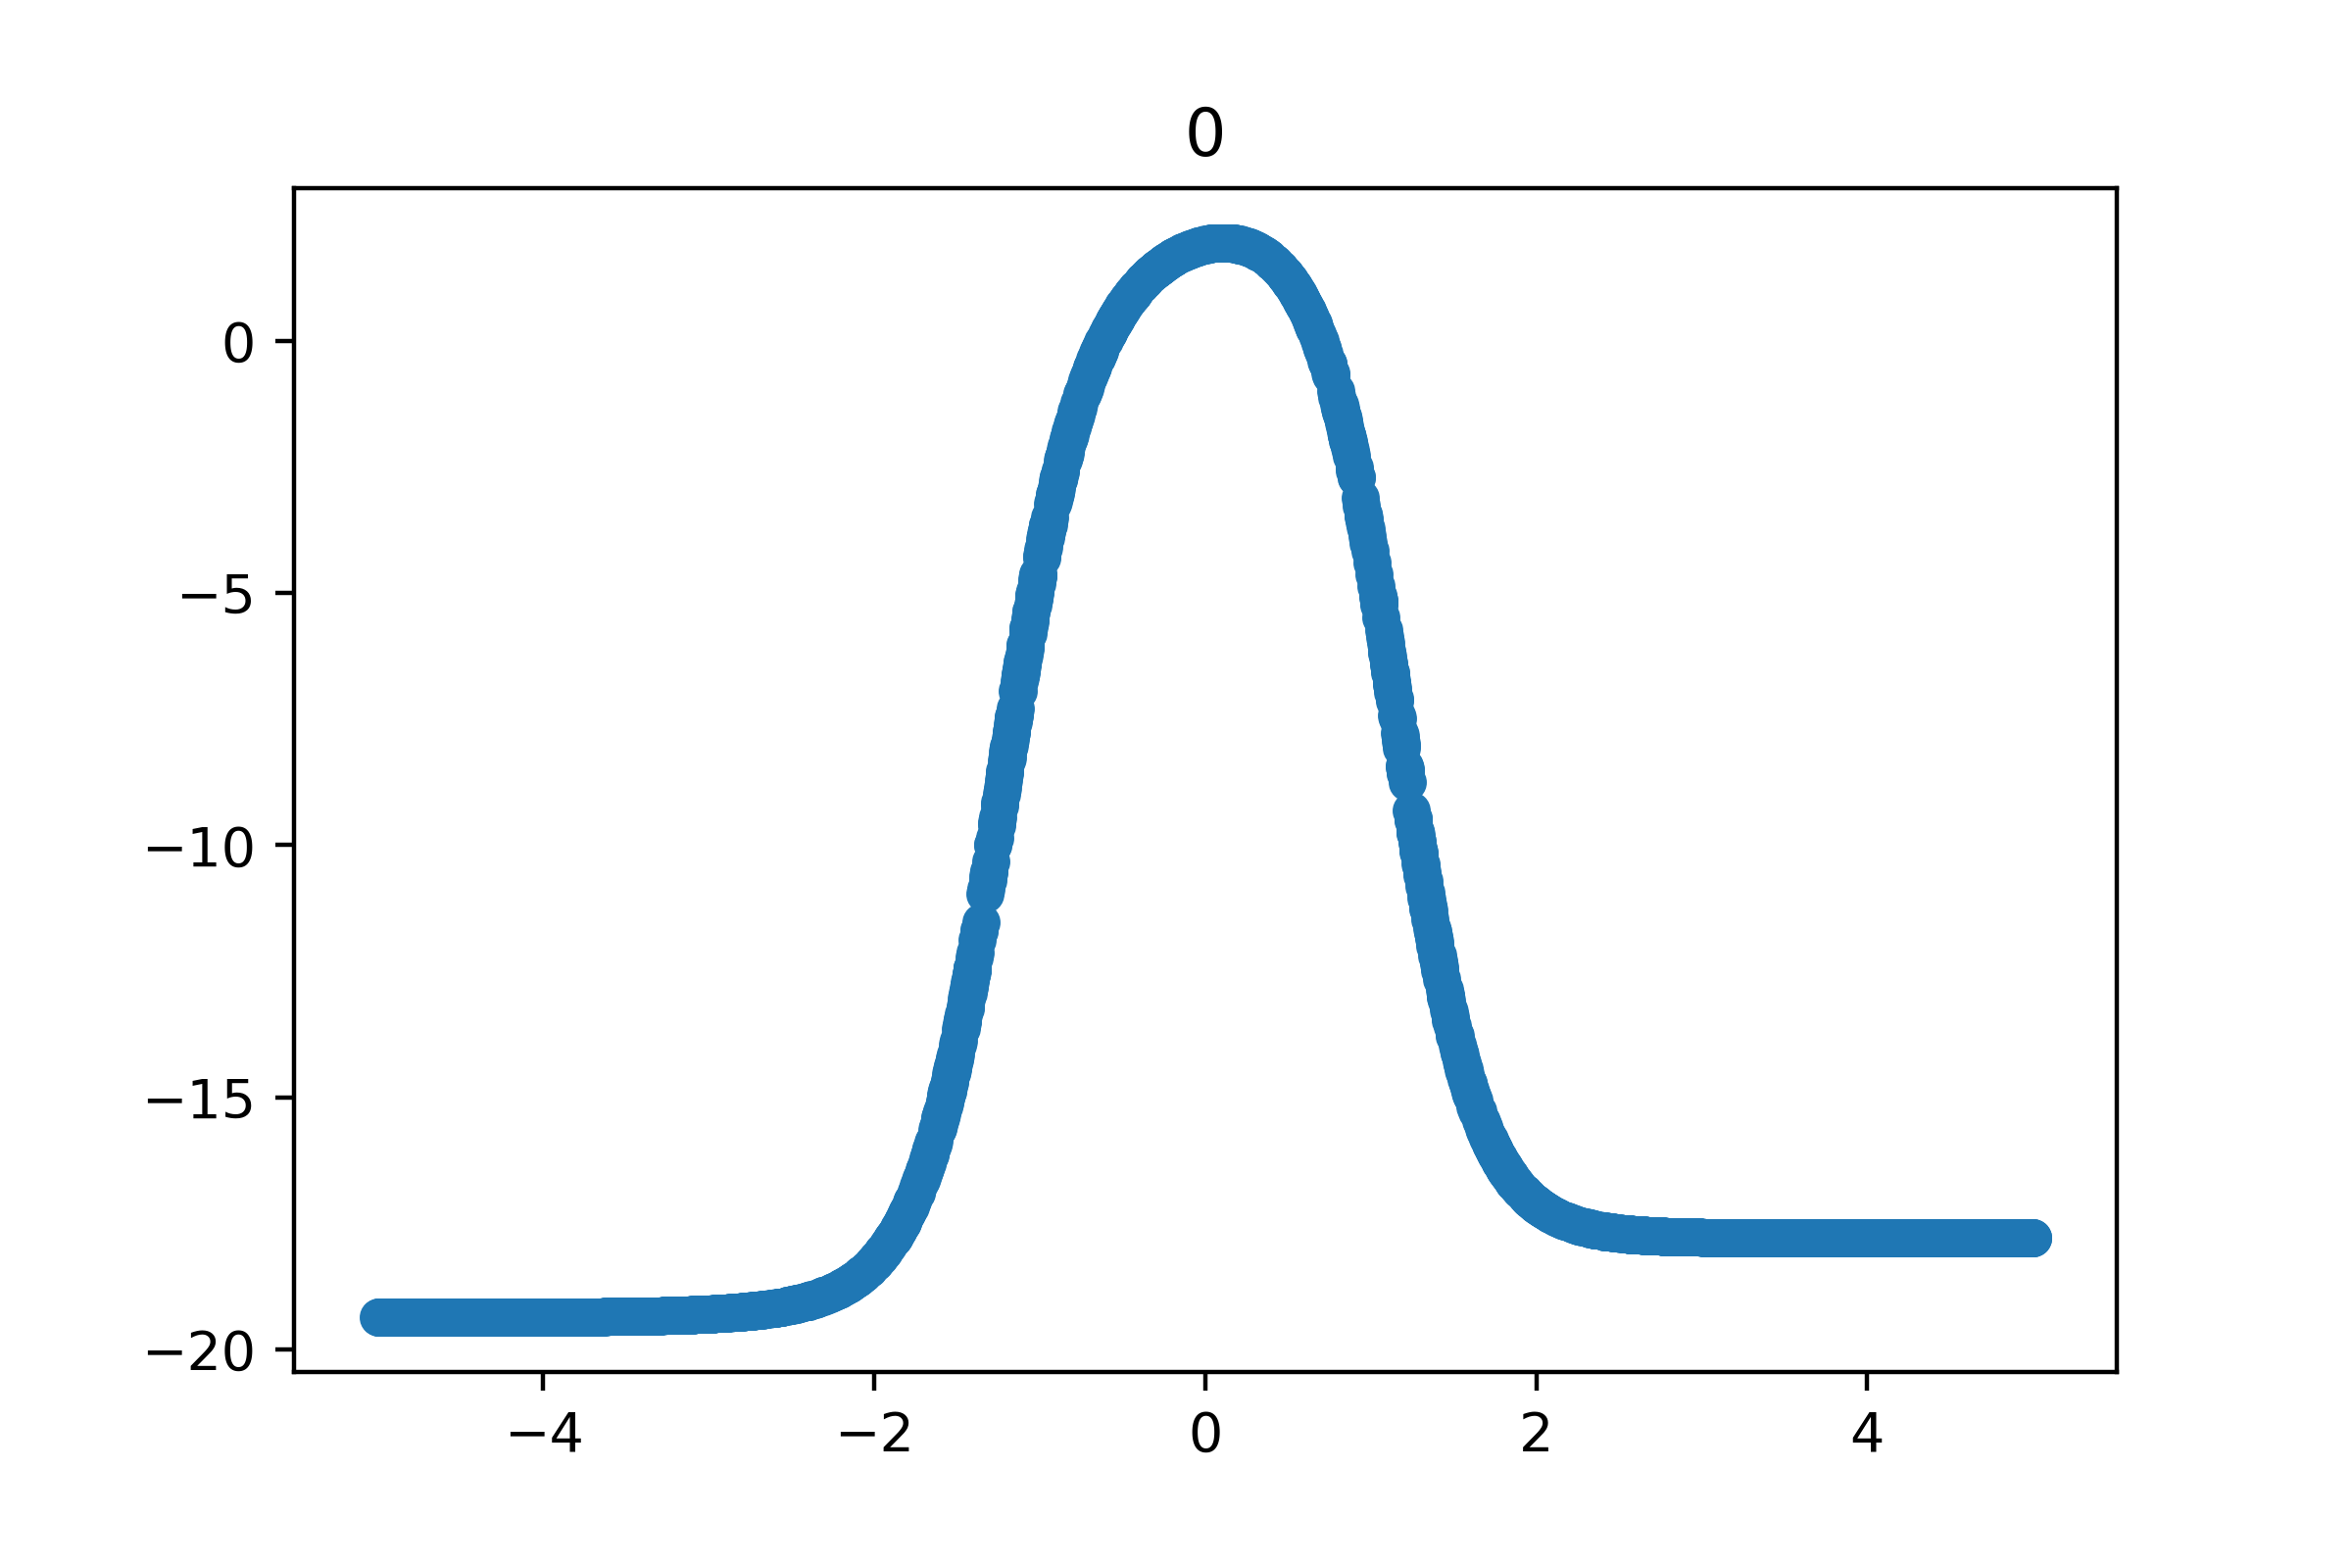
\includegraphics[width=0.40\textwidth]{fig/mnl/ci1.png} &
%     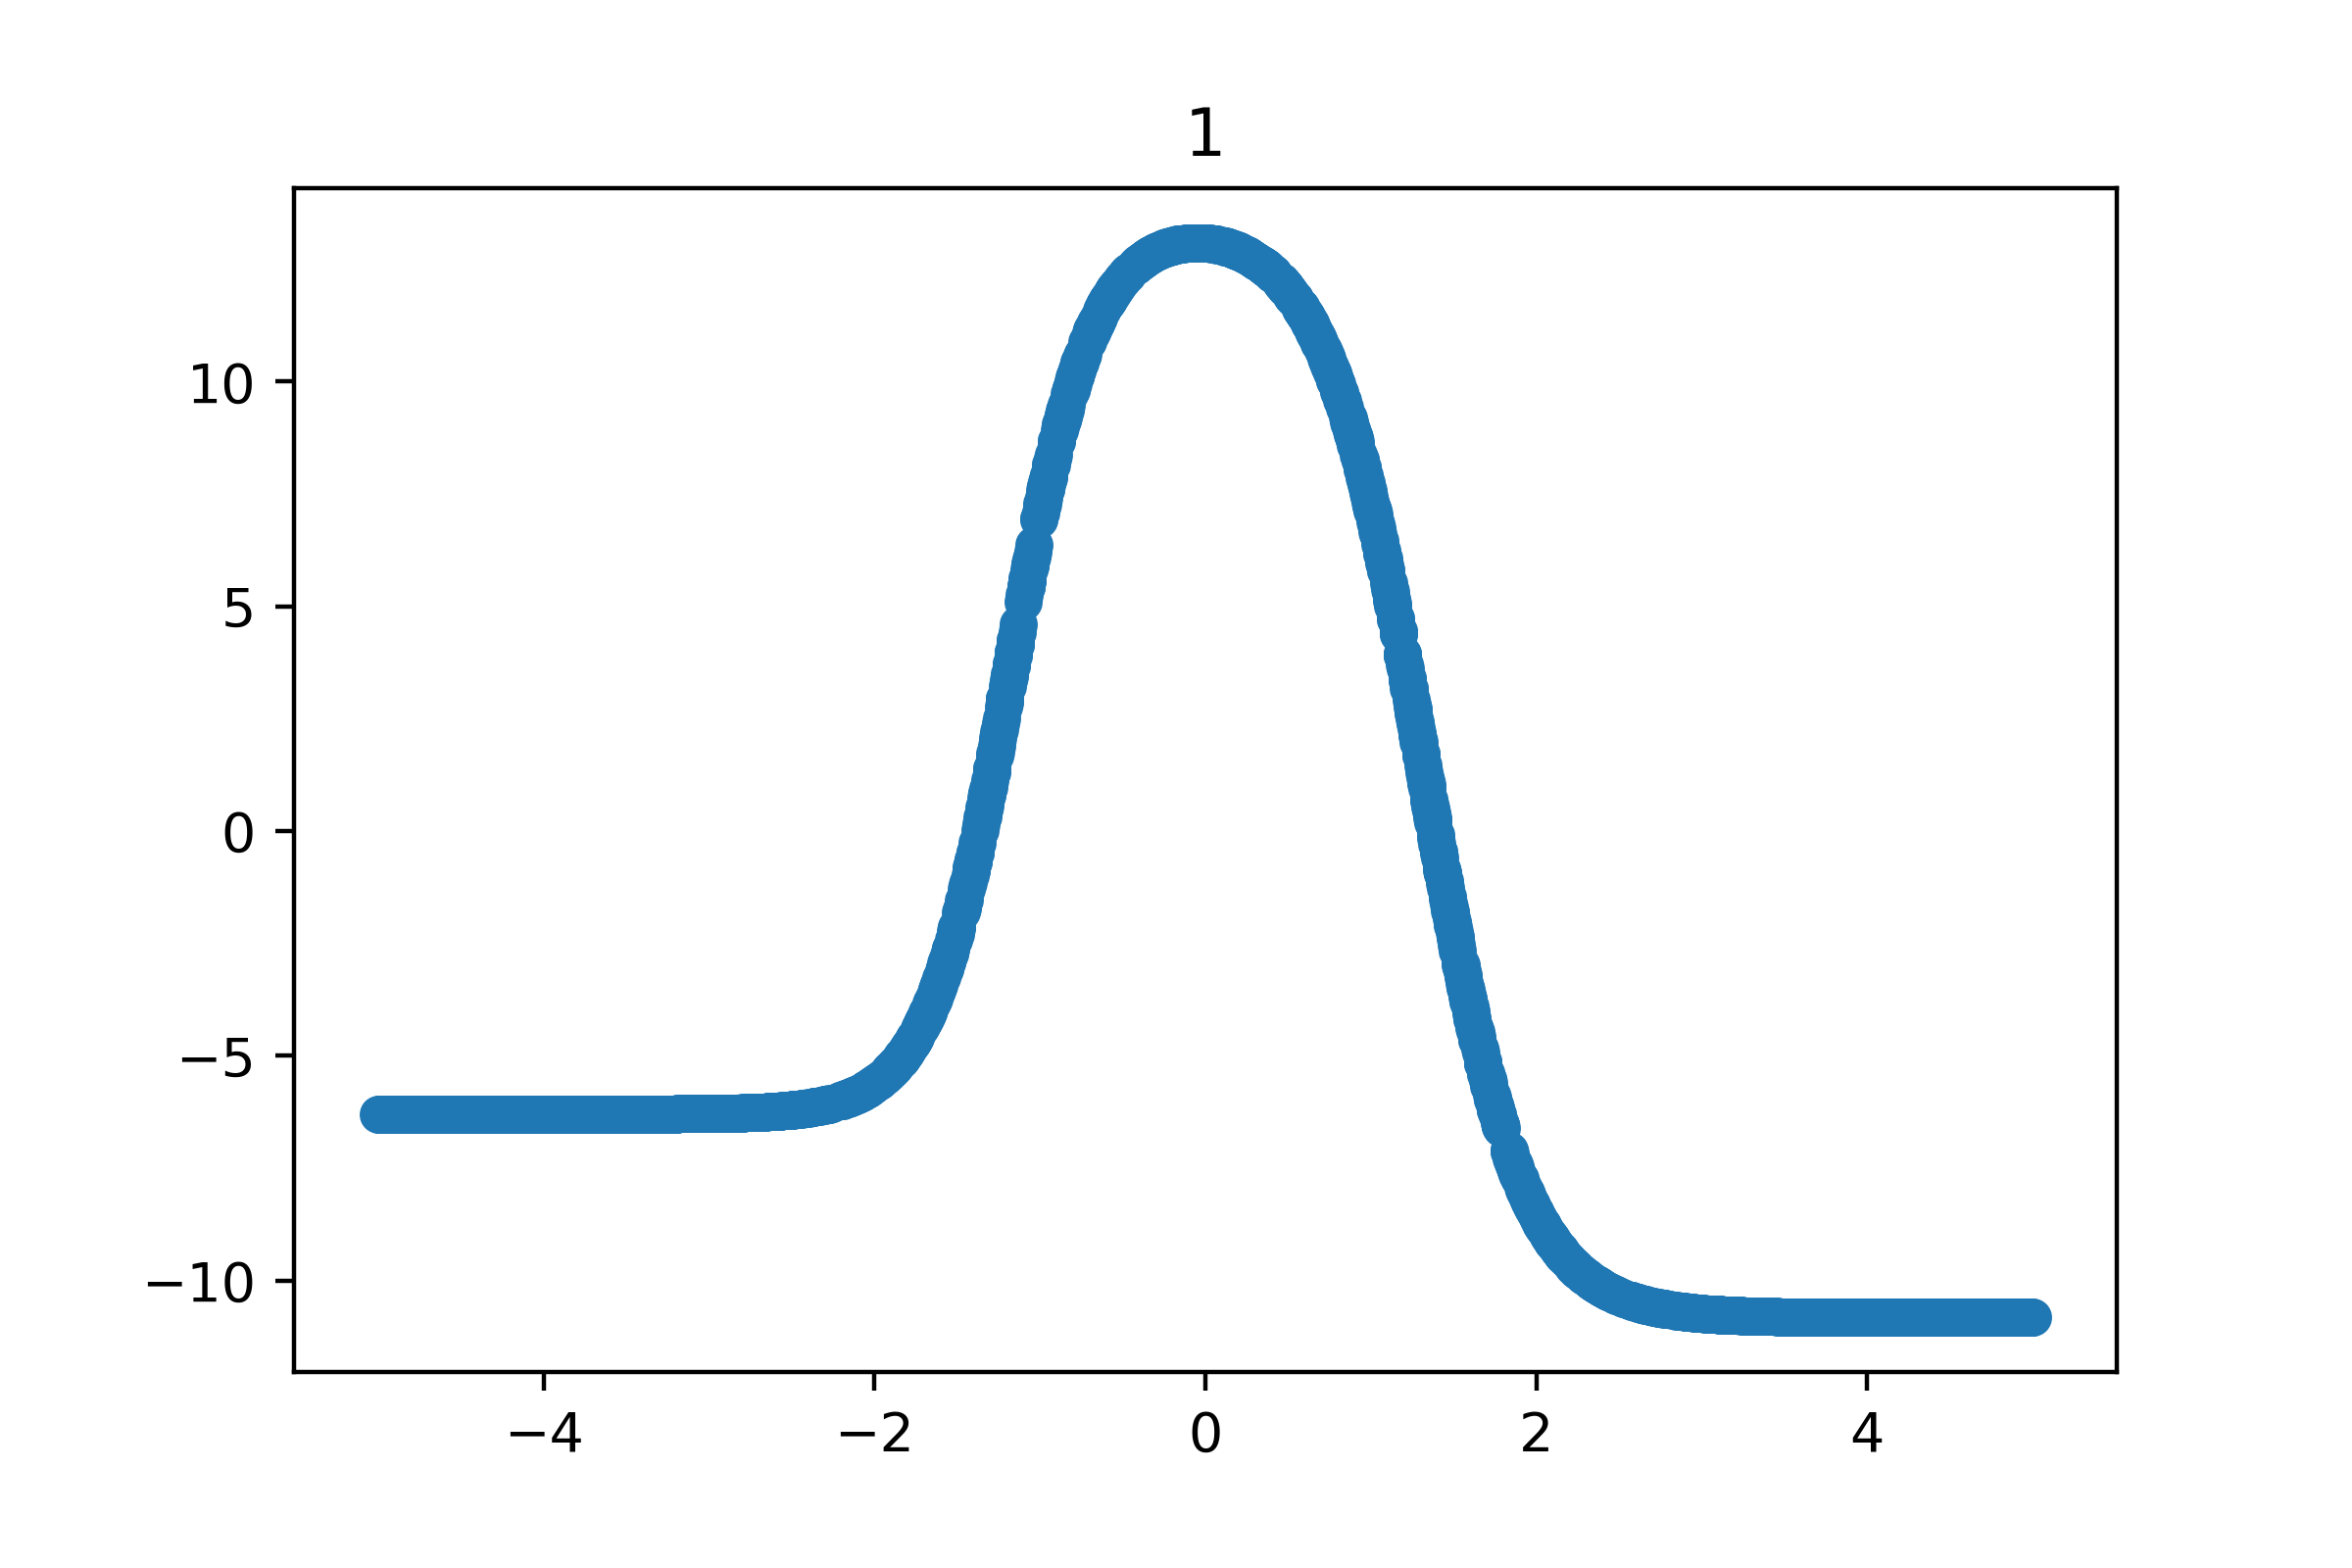
\includegraphics[width=0.40\textwidth]{fig/mnl/ci2.png}\tabularnewline
    
%     Ellipse & 
%     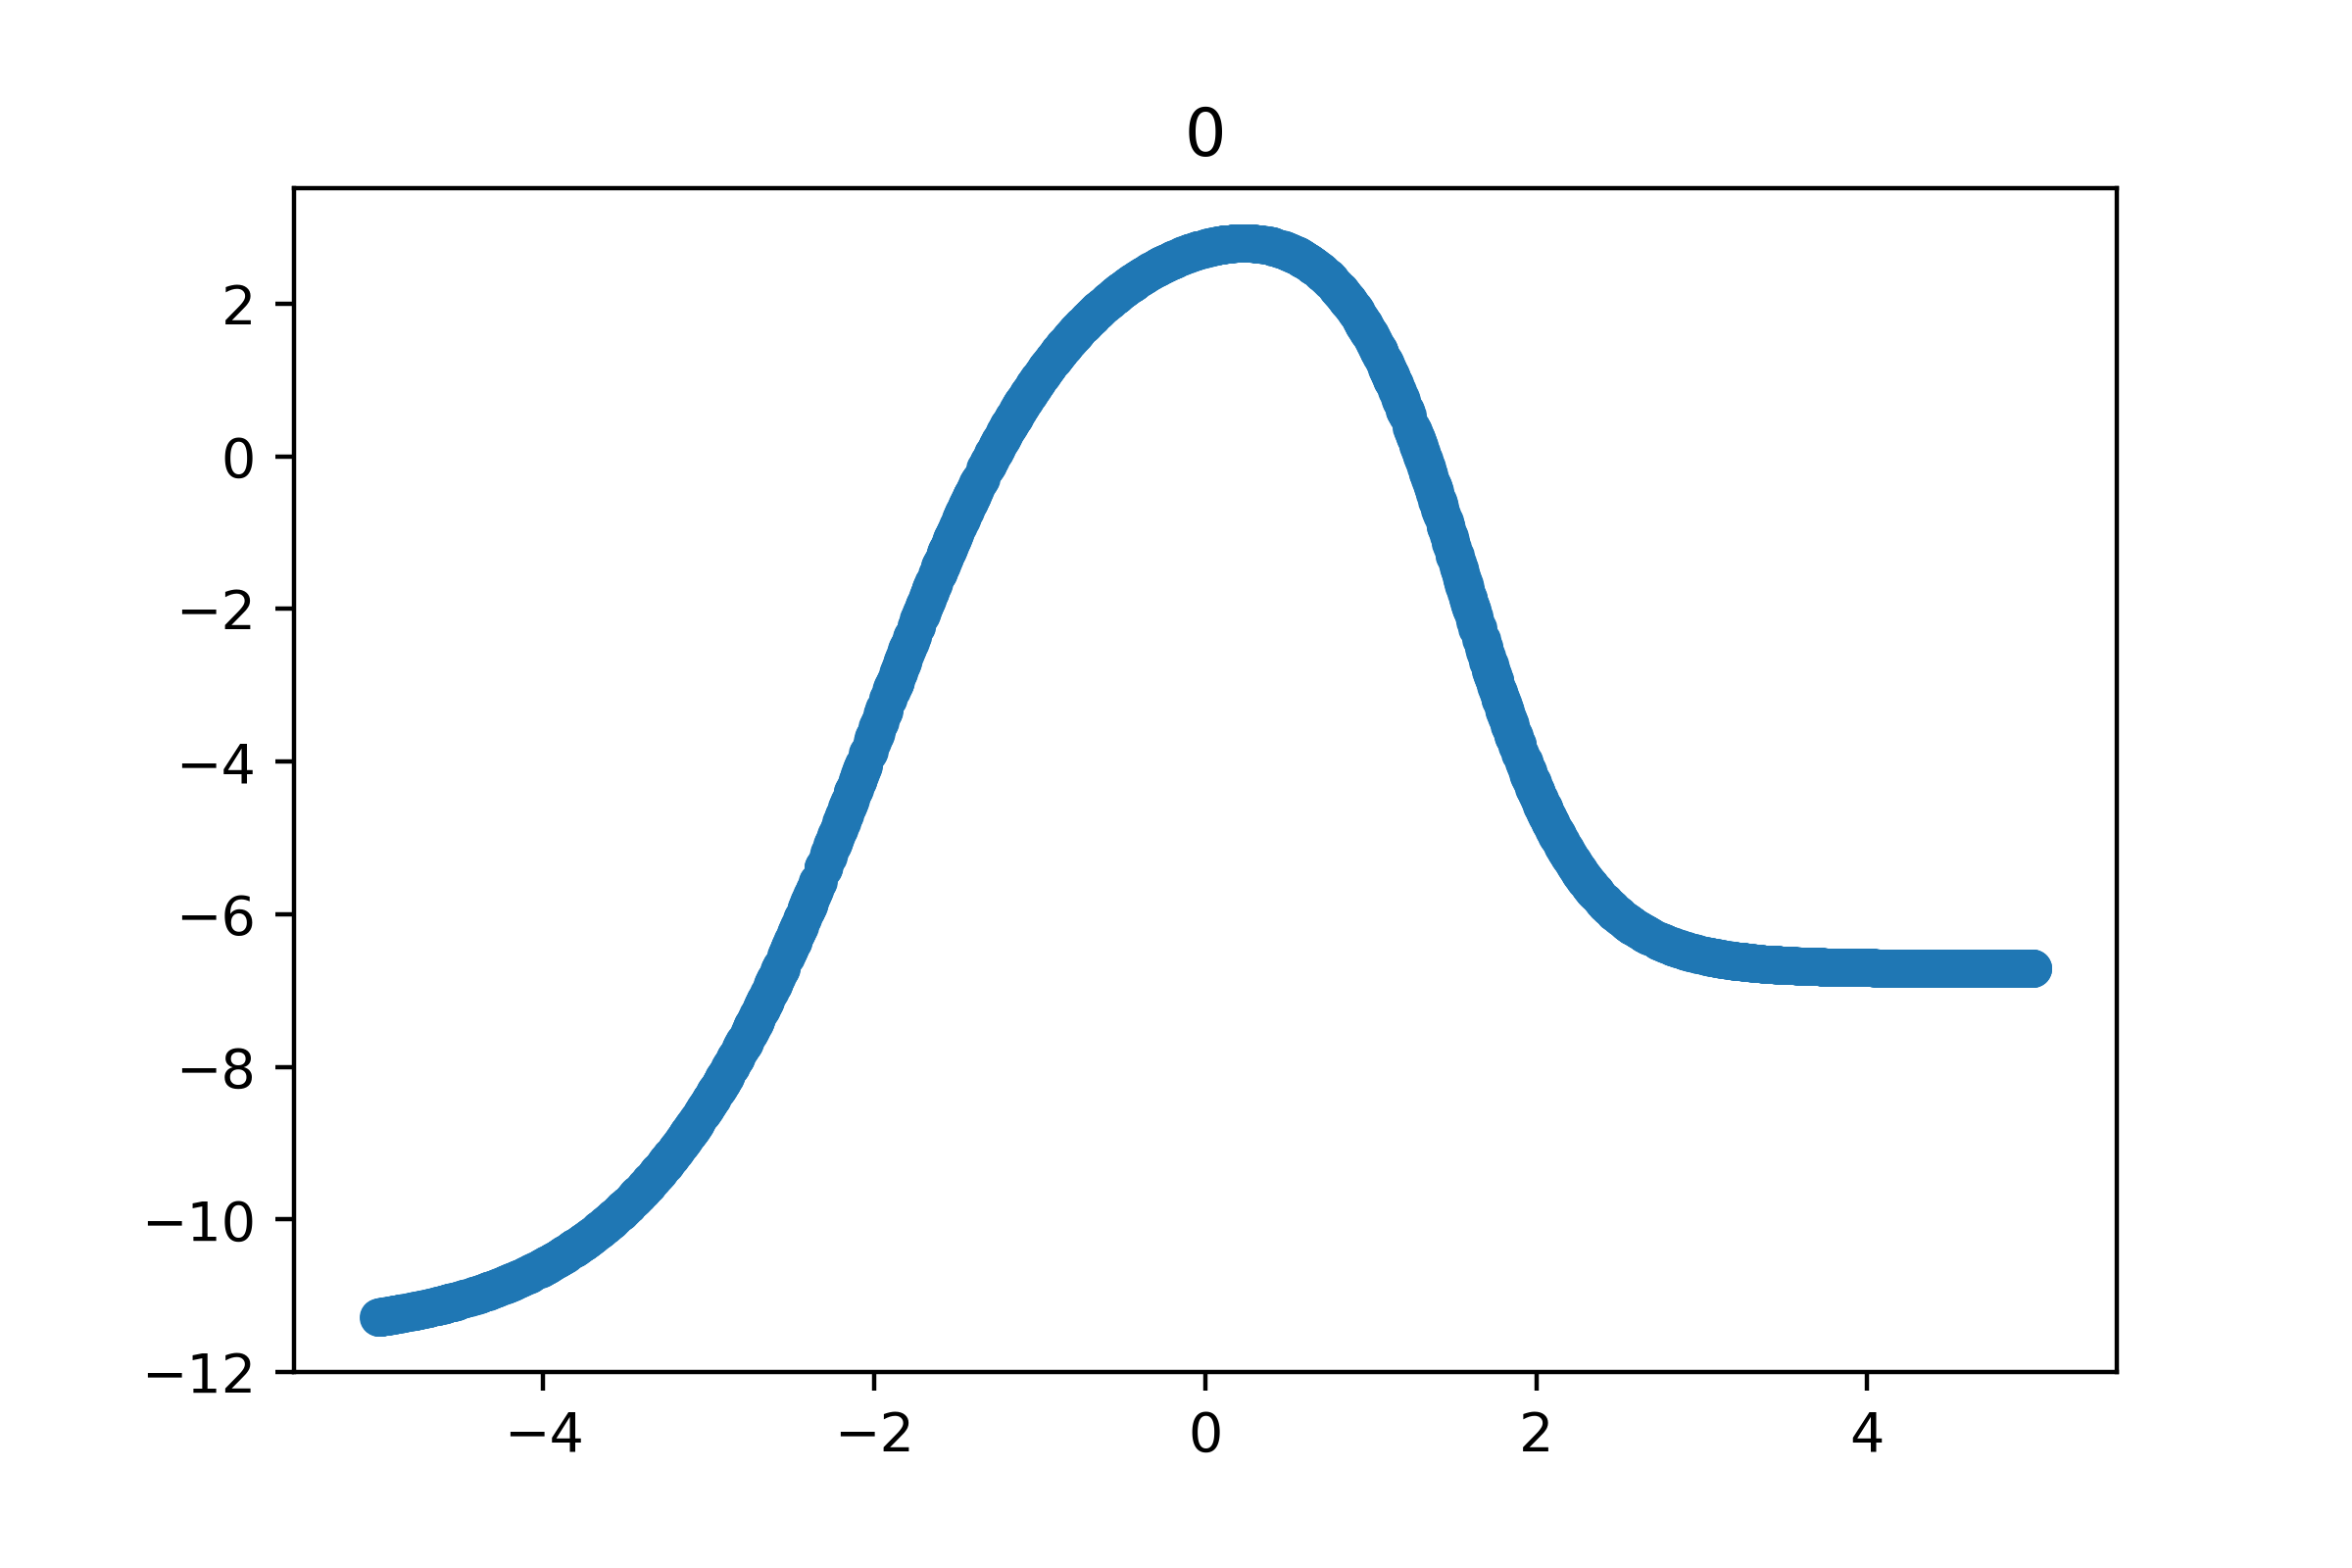
\includegraphics[width=0.40\textwidth]{fig/mnl/el1.png} &
%     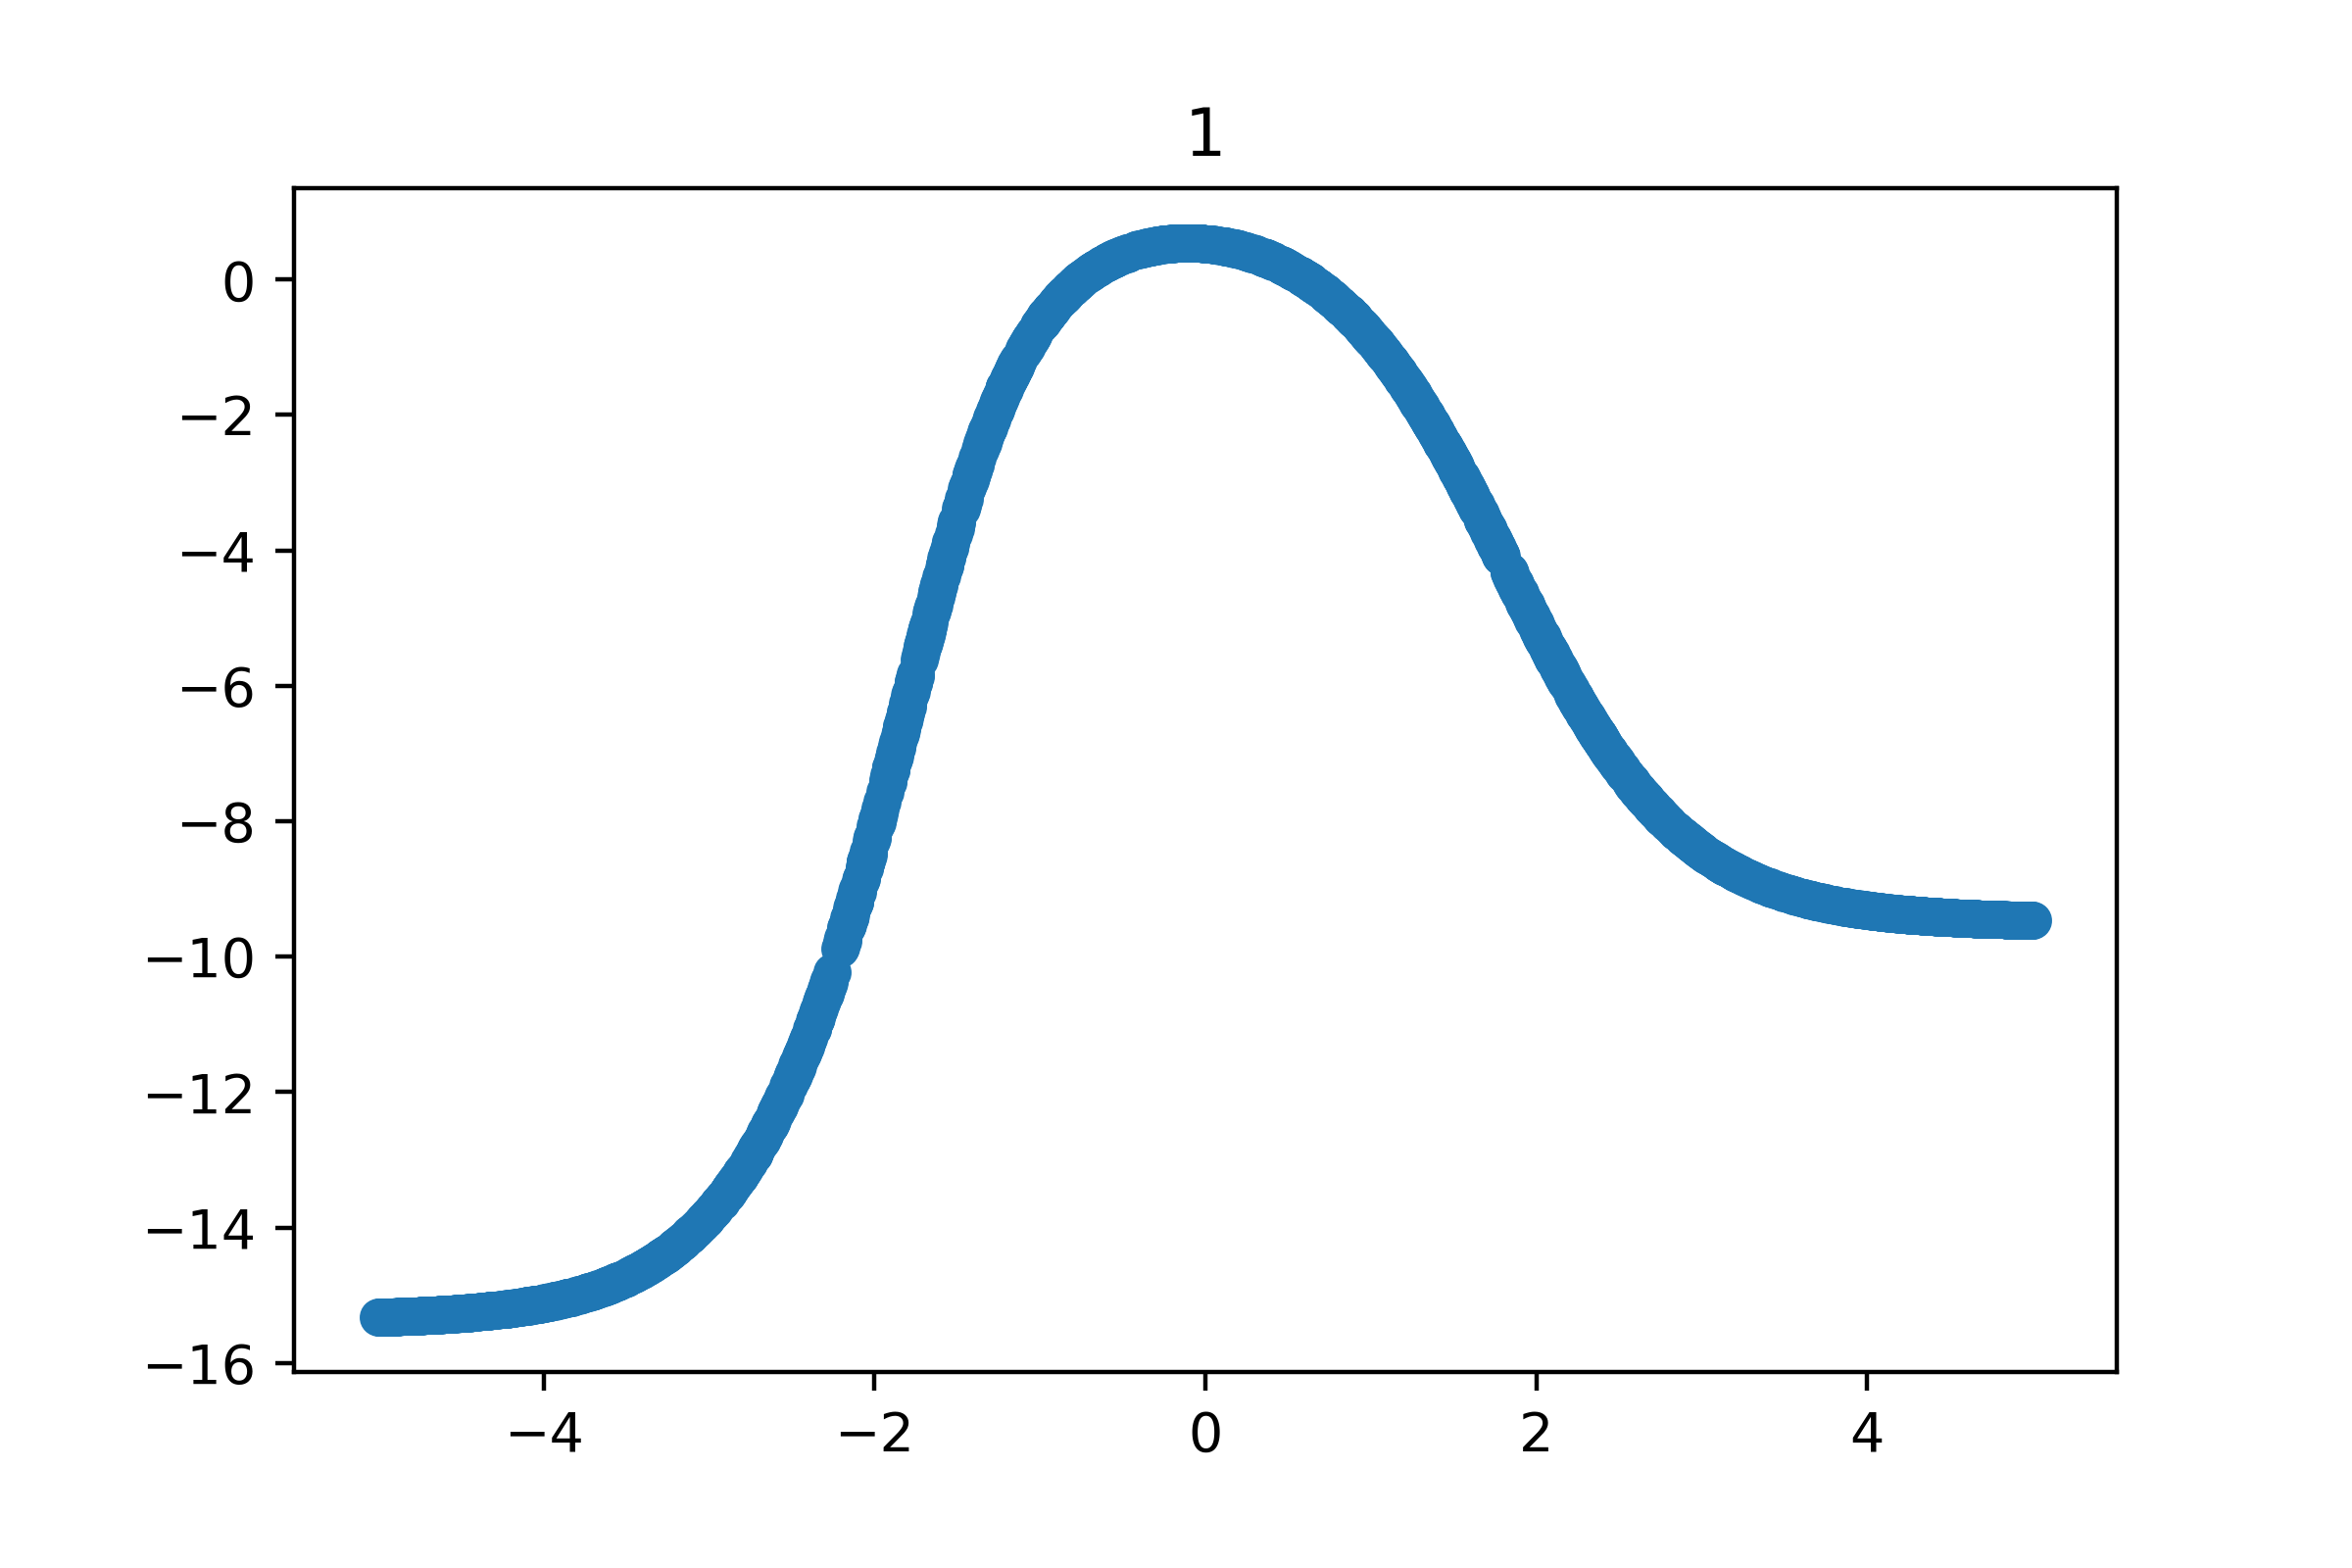
\includegraphics[width=0.40\textwidth]{fig/mnl/el2.png}\tabularnewline
    
%     XOR & 
%     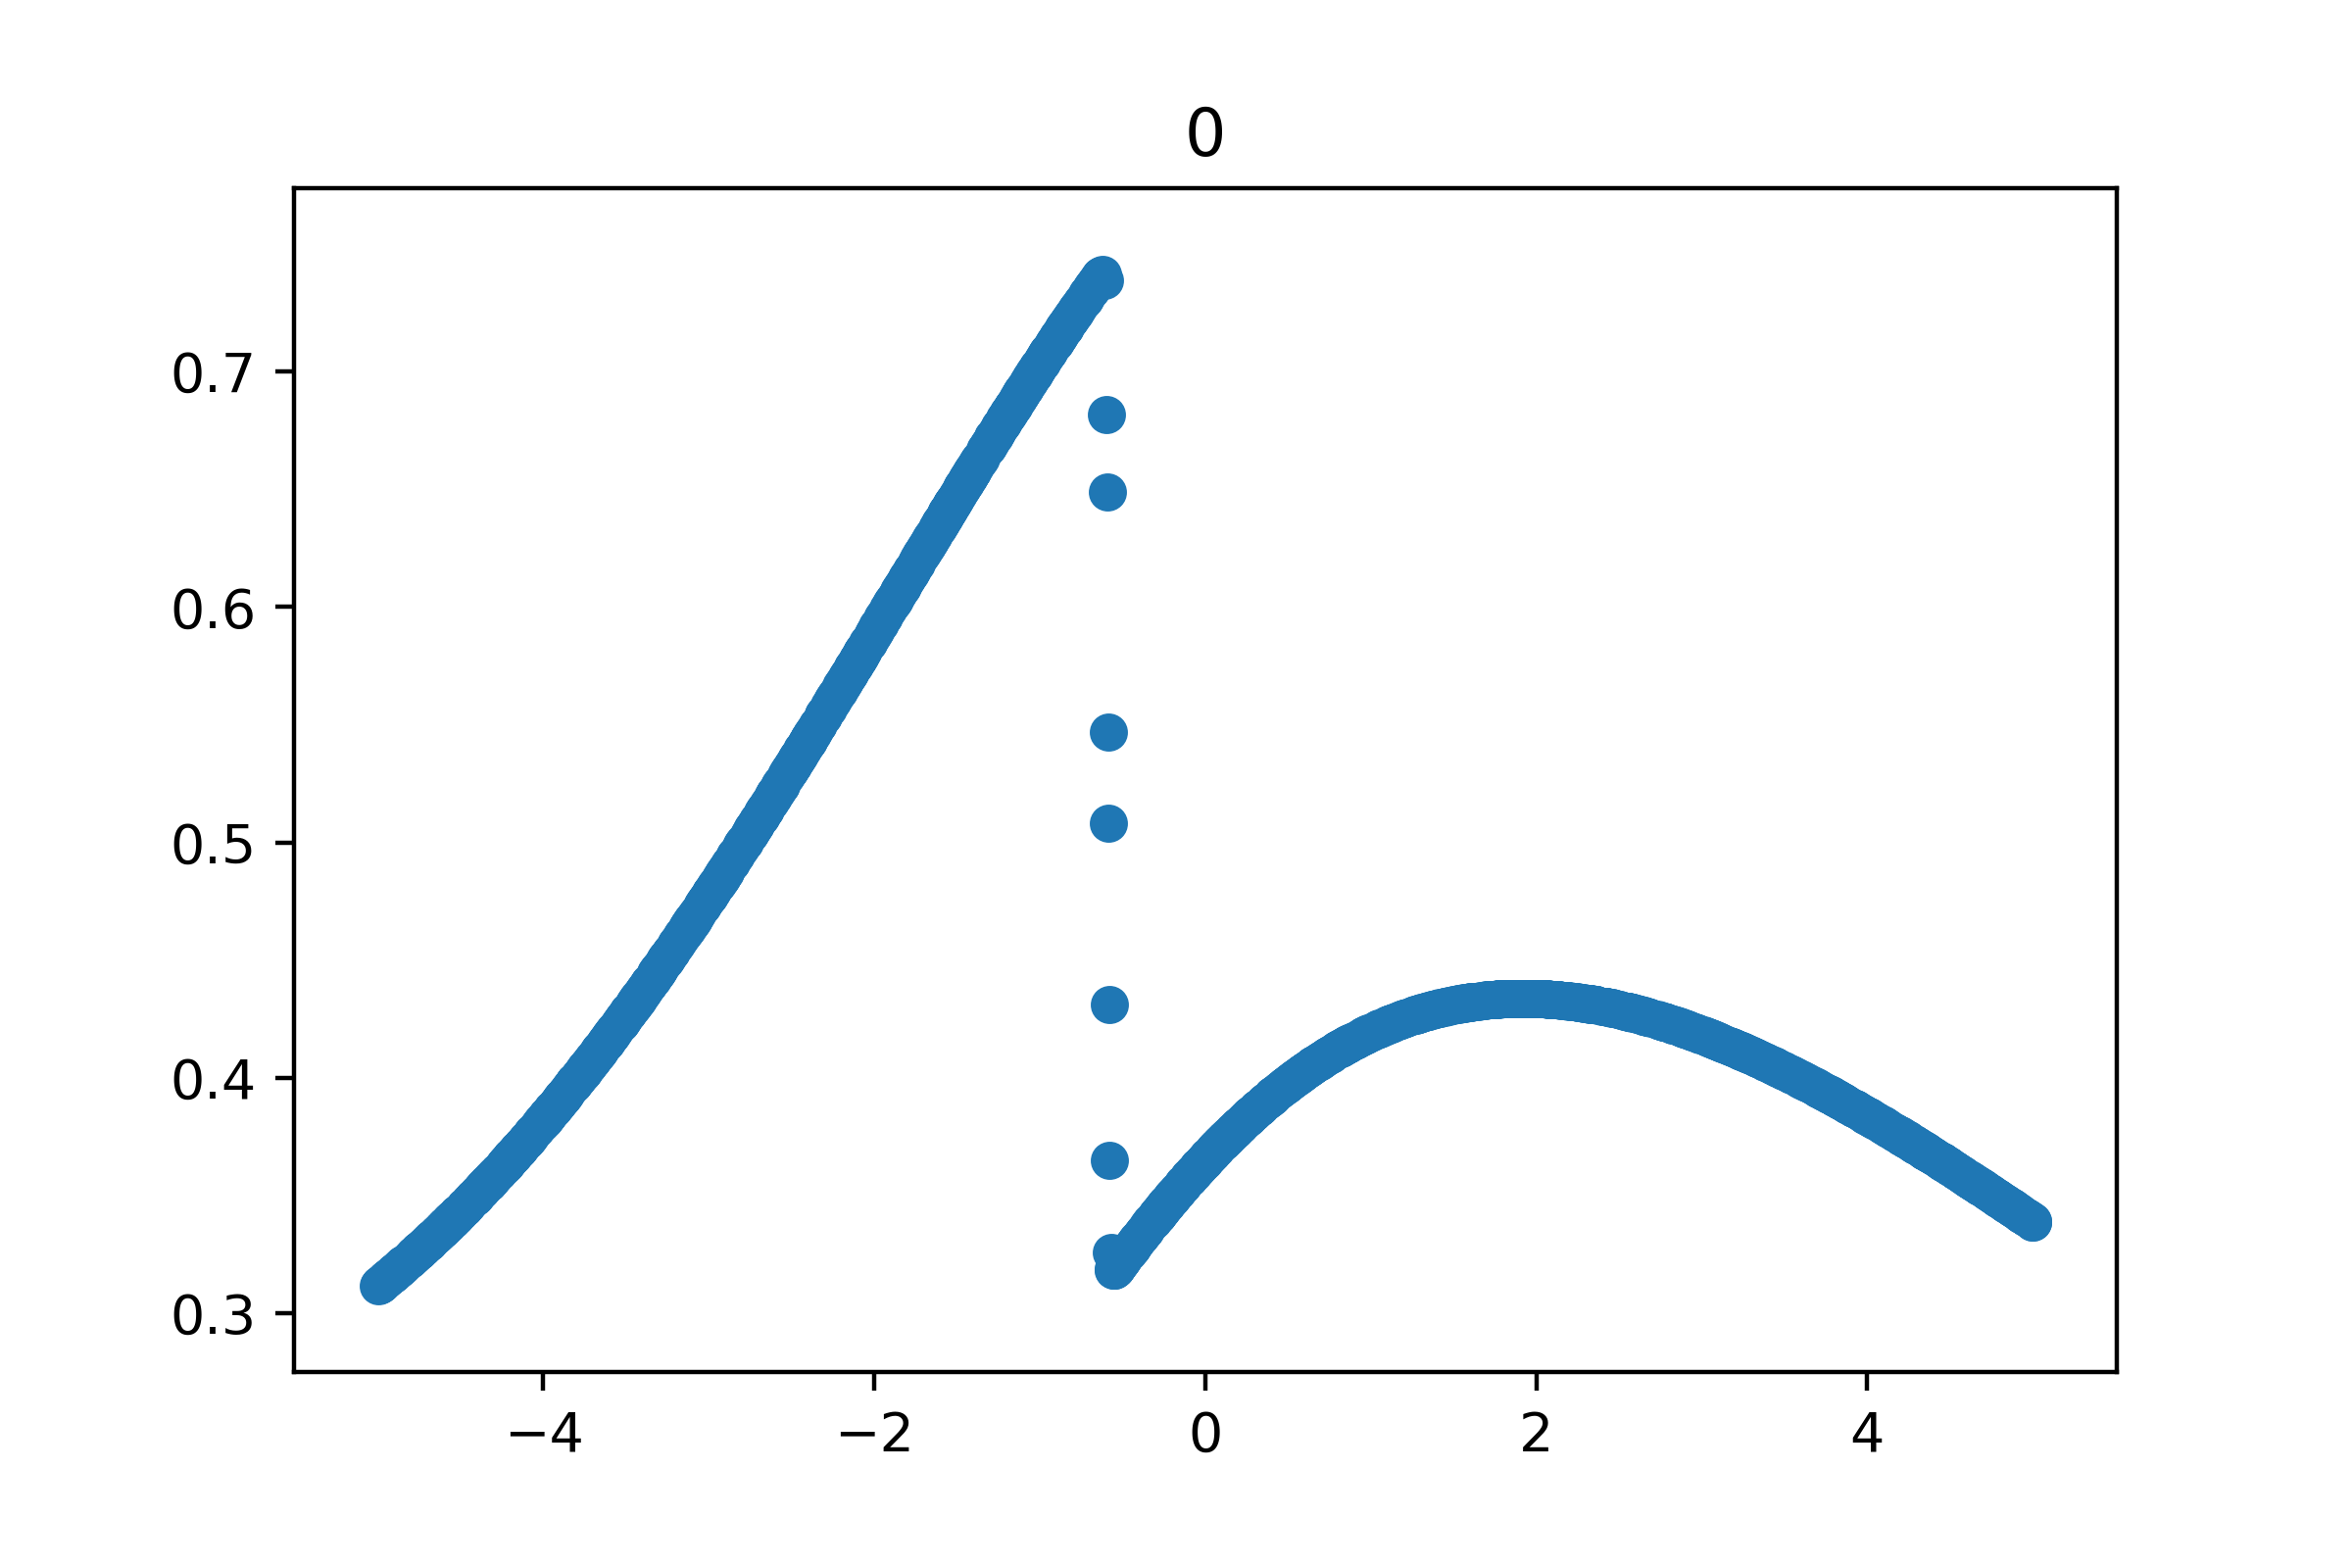
\includegraphics[width=0.40\textwidth]{fig/mnl/xr1.png} &
%     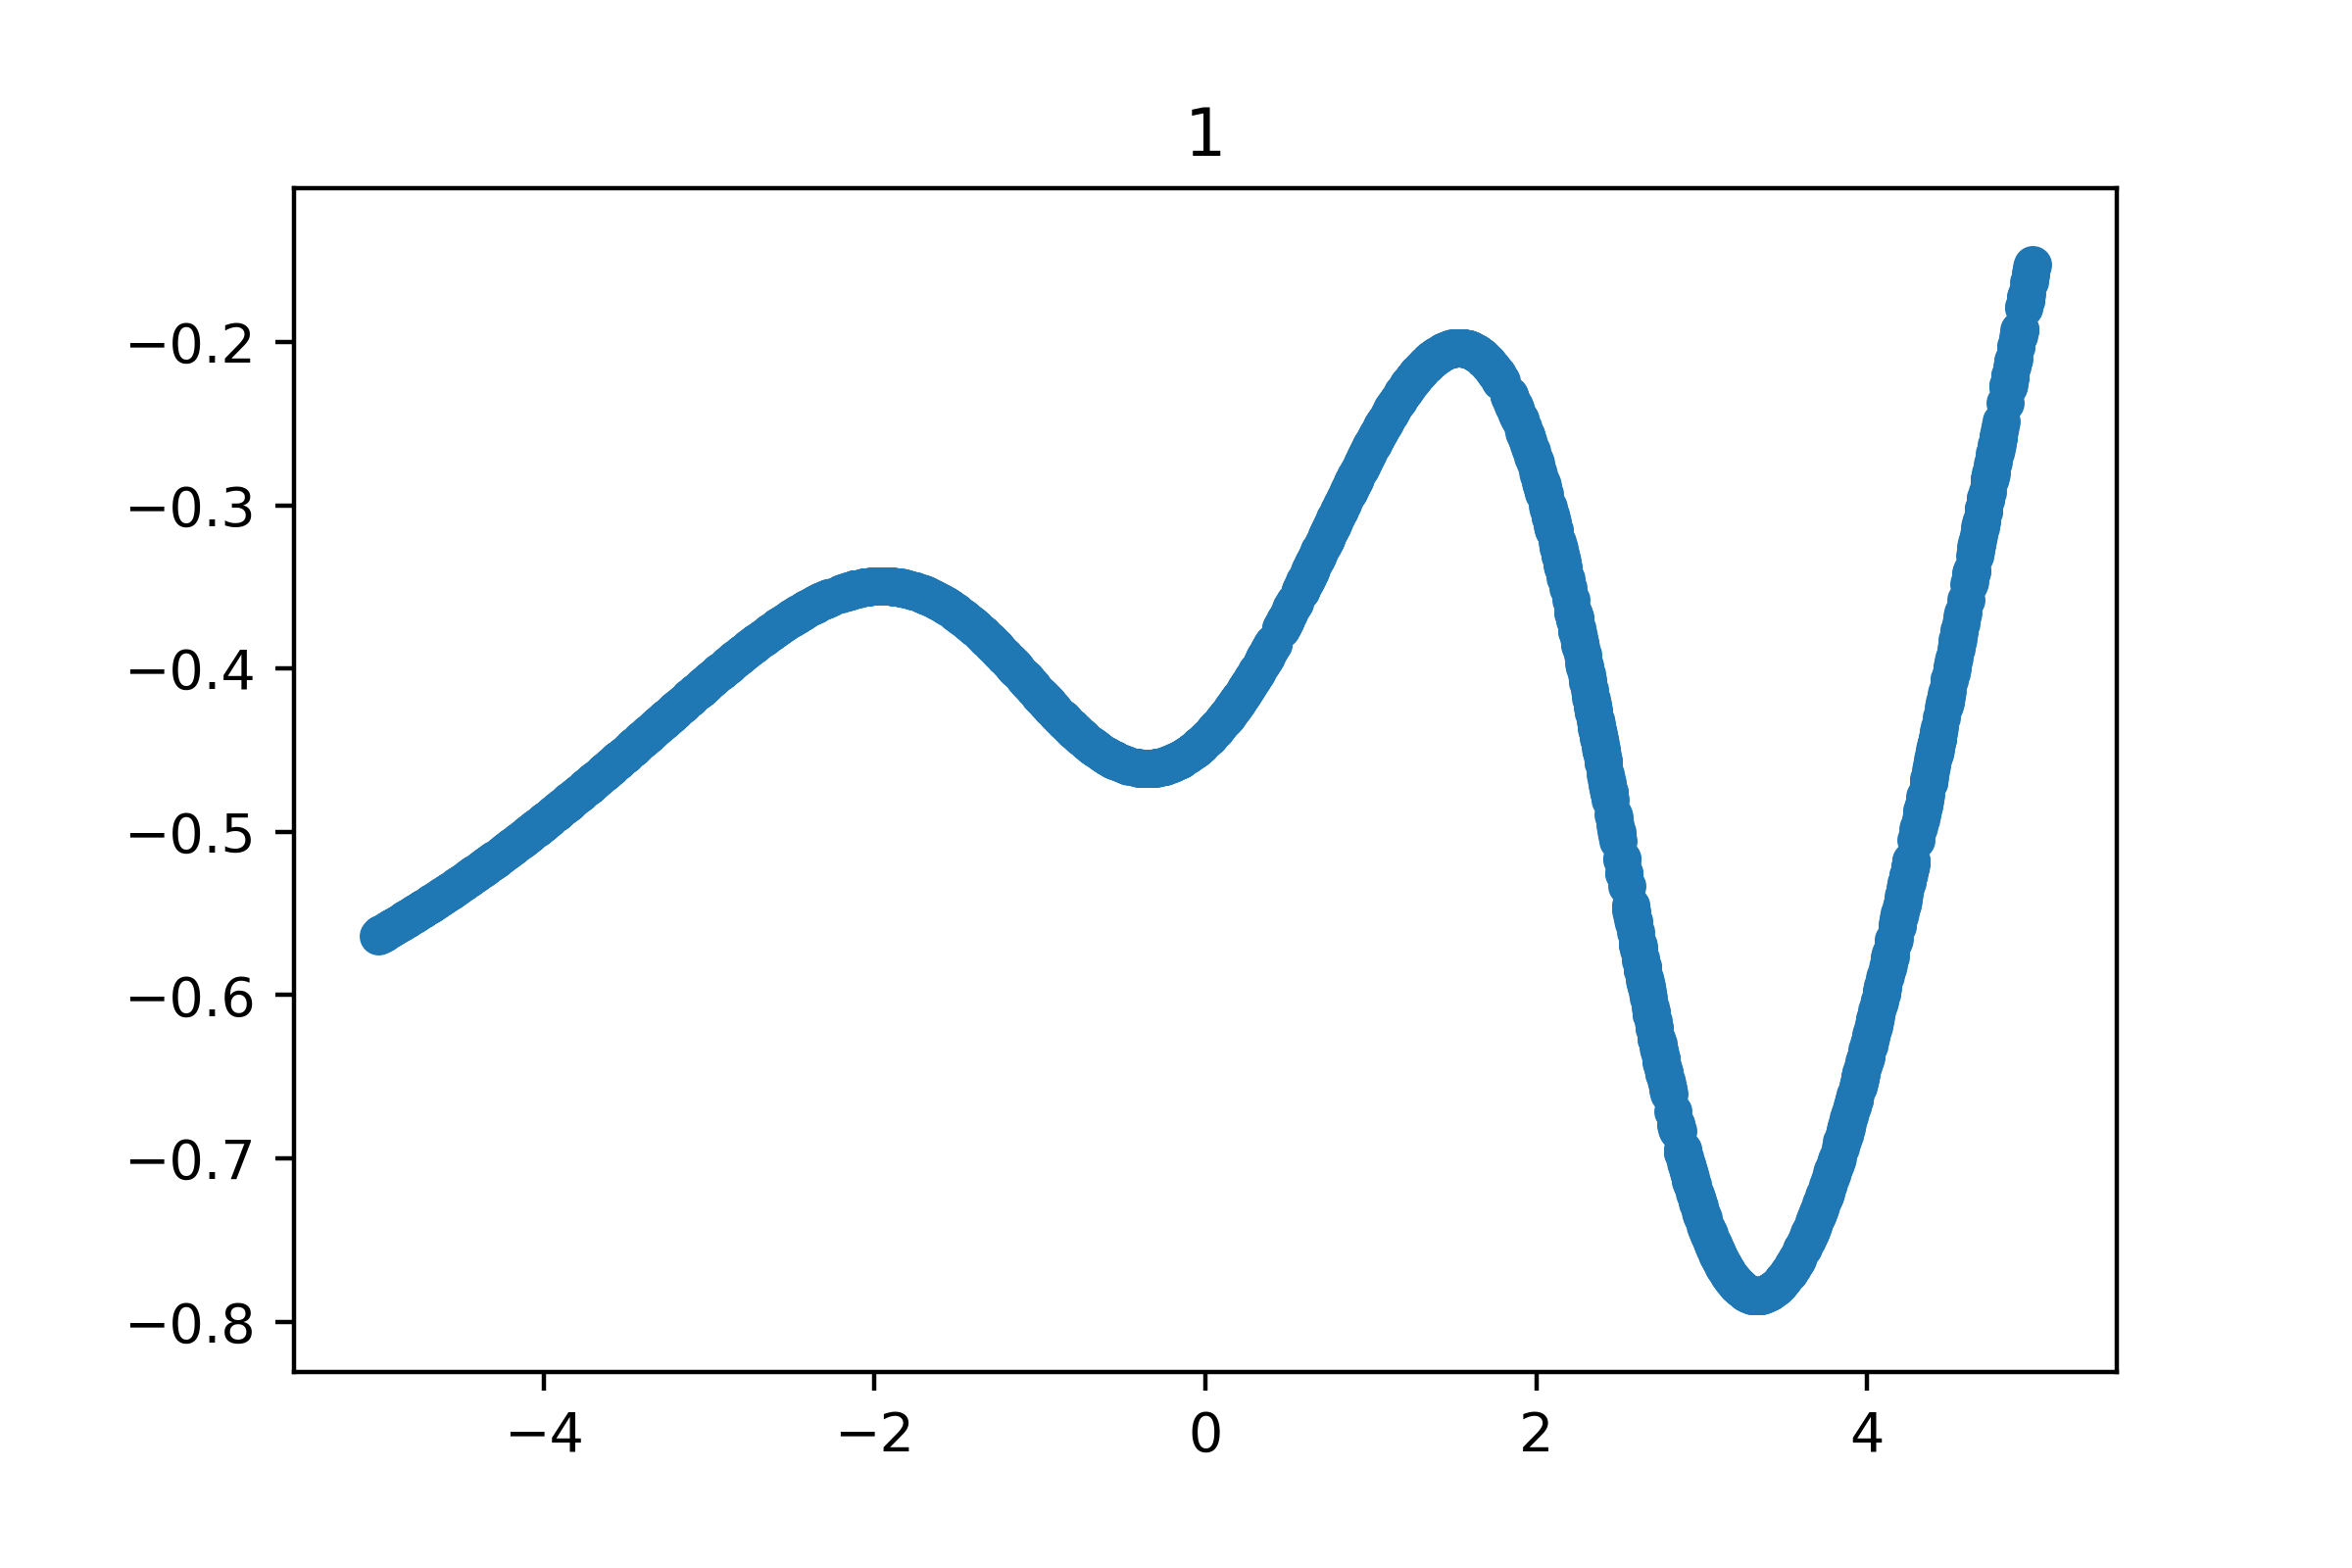
\includegraphics[width=0.40\textwidth]{fig/mnl/xr2.png}\tabularnewline
    
%     \bottomrule
    
%     \caption{}

% \end{longtable}

\subsection{Analysis}

\paragraph{Circle:} True to its name, the circle dataset contains a circle of true positives encased in a field of true negatives. Our architecture performs well in this dataset, achieving an f1 score of 0.9903. GBMs perform slightly worse, with an f1 score 0.8824, due to mild over-fitting on the edges of the circle. This dataset is not linearly separable, so logistic regression performed poorly, with an f1 score of 0.0000. 

This dataset demonstrates one of the unexpected advantages of our power-reduced neural network architecture. By removing the joint terms from the network, we've reduced the number of  weights our network needs to fit by an order of $n$ when compared to an equivalently sized fully-connected layer. This reduction helps curb over-fitting, allowing the network to perform better without applying additional regularization constraints, such as dropout \citep{Srivastava2014Dropout:Overfitting}.


\paragraph{Ellipse:} The ellipse dataset is similar to the circle dataset, but with a correlation of 0.5 between the $x_1$ and $x_2$ variables. Our network performance falls significantly to 0.8113 as the method is unable to handle correlations between input variables. GBMs perform almost identically with a score of 0.8654, while logistic regression performs poorly with an F1 score of 0.0000.

This dataset illustrates the major downside of our network architecture and other GAM-like approaches. While the network is capable of handling the circle, the addition of correlation term $x_1 x_2$ creates a behavior that cannot be modeled, resulting in a major loss of accuracy. This issue applies to all behavior that cannot be modeled as a linear combination of univariate functions, and can lead to decreased accuracy, as in this example, or a complete failure to fit, as in the XOR dataset. 


\paragraph{XOR:} The XOR dataset mimics a famous neural networks problem, where the goal is to classify points in quadrants one and three as class one and points in quadrants two and four as class two. Our architecture is completely unsuited for this task, and achieves a similar f1-score to logistic regression. While possible to model one of the four quadrants, joint terms are required to model both, so more powerful methods like GBMs will perform much better on this type of problem.

These limitations help explain why GAMs and GAM-like architectures have not risen to prominence in most mainstream machine learning applications. When compared to more powerful techniques like fully-connected neural networks or tree-based ensembles, this architecture seems woefully under-powered, failing to achieve valid predictions for even these very simple problems. However, the improved interpretability of this method still warrants attention, and the question remains: how much do joint terms matter in real-world classification tasks? 
